%%%%%%%%%%%%%%%%%%%%%%%%%%%%%%%%%%%%%%%%%
% Lachaise Assignment
% LaTeX Template
% Version 1.0 (26/6/2018)
%
% This template originates from:
% http://www.LaTeXTemplates.com
%
% Authors:
% Marion Lachaise & François Févotte
% Vel (vel@LaTeXTemplates.com)
%
% License:
% CC BY-NC-SA 3.0 (http://creativecommons.org/licenses/by-nc-sa/3.0/)
% 
%%%%%%%%%%%%%%%%%%%%%%%%%%%%%%%%%%%%%%%%%

%----------------------------------------------------------------------------------------
%	PACKAGES AND OTHER DOCUMENT CONFIGURATIONS
%----------------------------------------------------------------------------------------

\documentclass{article}

\input{structure.tex} % Include the file specifying the document structure and custom commands

\usepackage{hyperref}

\usepackage{siunitx}

\usepackage{xcolor} % to color the conversation to look better

\usepackage[utf8]{inputenc} % Required for inputting international characters
\usepackage[T1, T2A]{fontenc} % Output font encoding for international characters

\usepackage[english,serbian]{babel}

\usepackage{amssymb}

\usepackage{multicol} % used for side by side equations
\usepackage{caption}
\captionsetup[table]{name=Табела}
\captionsetup[figure]{name=Слика}

\usepackage{physics}
\usepackage{derivative}


\newcommand{\rom}[1]{\uppercase\expandafter{\romannumeral #1\relax}}
%----------------------------------------------------------------------------------------
%	ASSIGNMENT INFORMATION
%----------------------------------------------------------------------------------------

\title{Основи физике полупроводника} % Title of the assignment

\author{Александар Вуковић} % Author name and email address

% \date{\today} % University, school and/or department name(s) and a date
% није на ћирилици

%----------------------------------------------------------------------------------------

\hyphenation{пре-да-ва-њи-ма те-ле-фон-ске ла-бо-ра-то-ри-ја-ма не-га-тив-ном раст-во-ри-ма кон-стан-ту}

\hyphenation{ком-пен-зо-ва-ног по-сто-ја-ти не-у-трал-ног ак-цеп-то-ра ек-ви-ли-бри-ју-ма гер-ма-ни-јум-ски по-лу-про-вод-ни-ку гер-ма-ни-ју-ма и-стра-жи-ва-ње не-чи-сто-ће кон-та-ми-на-ци-је по-ја-ча-ва-ча по-лу-про-вод-ник на-е-лек-три-са-ње прик-ључ-ка пла-ни-ра-ни прет-ва-ра-ју и-лу-стро-ва-но ос-ци-ло-ско-па прик-љу-ча-ка е-лек-тро-не ква-зи-че-сти-ца јед-но-став-н е-лек-тро-ни јед-но-став-не прав-ље-ни до-нор-ских ин-те-рак-ци-ја за-до-во-ља-ва ју-ће ком-пен-зо-ва-ни прик-лад-но ек-ви-ва-лент-не кон-цен-тра-ци-ја е-лек-тро-ста-тич-ки при-ка-зане-лек-тро-ста-тич-ког по-тен-ци-ја-ла јед-на-чи-ном ди-фе-рен-ци-јал-на кон-так-ти-ма ек-ви-либ-ри-јум ек-ви-ва-лент-но тран-зи-сто-ру са-ту-ра-ци-је ка-па-ци-тив-но-сти оп-то-е-лек-трон-ских е-фи-кас-но-сти ин-тер-пре-та-ци-ја и-лус-тро-ван е-лек-тро-ни-ке ис-прав-ља-чких по-лу-про-вод-ни-ка прак-тич-ном ис-ко-рис-ти-ти те-ле-фон-ских у-да-ље-ност стра-не по-лу-про-вод-ни-ци ис-тра-жи-ва-ња про-во-ђе-ње шуп-љи-на кон-цен-тра-ци-о-ном на-прав-ље-ни у-ни-вер-зи-те-та по-лу-про-вод-нич-ких а-на-ло-ги-ју ис-тра-жи-вач-ког ин-ду-ко-ва-на прос-тор---на-е-лек-три-са-ња о-бе-ћа-ва-ју-ће шуп-љи-не о-со-би-на-ма про-гра-ма те-о-рет-ска pо-ја-ча-њем на-прет-ком на-е-лек-три-са-ња по-ве-ћа-ни ре-ком-би-на-ци-ју вре-мен-ског про-ду-же-ног вре-мен-ско из-ме-ри-ти ге-не-ра-ци-је ка-та-ли-зује е-лек-трон-ских по-ре-ме-ћа-ја крис-та-лу ге-не-рал-но по-лу-про-вод-ни-чког Но-бе-ло-ве ду-го-роч-н Те-ле-фон ве-о-ма при-сут-ној ап-со-лут-ној и-ма-ју ди-ја-мант-ску ди-е-лек-трич-ном е-нер-гет-ских е-нер-гет-ски ду-го-роч-на не-га-тив-ним фор-ми-ра-ју тер-мал-ном сли-ци по-ве-за-на гер-ма-ни-ју-му кри-ста-ли-ма по-сма-тра-њу кван-ти-та-тив-на слич-но-сти ко-ли-чи-не е-лек-тро-на тран-зи-сто-ра е-лек-трон-ски слу-ча-ју е-лек-тро-ста-тич-ког под-ра-зу-ме-ва-ју-ћи до-би-ја ди-фу-зи-о-но ди-ја-гра ка-па-ци-те-том по-вр-шин-ских при-пи-сан не-га-тив-но екс-пе-ри-мент е-лек-трич-ног нај-јед-но-став-ни-је пред-ло-же-на ди-ја-грам са-др-жи прав-ље-ња прин-ци-пи-јел-ност а-ку-му-ла-ци-о-ну рав-но-те-жи си-сте-мат-ска ак-цеп-тор-ских пред-ви-ђе-но ди-фу-зи-јом про-ме-не ус-пеш-но тре-ти-ра-њем но-си-о-ци тран-зи-стор-ског ек-ви-либ-ри-ју-му ко-ри-сти-ли по-зи-тив-ни}

\begin{document}

\maketitle % Print the title

%----------------------------------------------------------------------------------------
%	Semiconductor research leading to the point contact transistor - Nobel Lecture
%----------------------------------------------------------------------------------------

% Стављено прво зато што друге две лекције говоре о накнадним истраживањима након открића транзисторског ефекта.

\section{Истраживање полупроводника које је довело до транзистора тачкастог контакта - Бардинов лауреат }

У овом предавању покушаћемо да опишемо идеје и експерименте који су довели до открића транзисторског ефекта отелотвореног у транзистору тачкастог контакта. Неки од важних истраживања су урађени после открића и биће описани у предавањима Шоклија и Братена. Као што ћемо видети, откриће је било велики корак унапред на путу истраживања полупроводника у коме су многи људи из различитих држава помогли. Зависило је и од добрих теоретских темеља већином изграђених 30-их година и напретку у уклањању нечистоћа из материјал, посебно германијума и силикона, 40-их година. Пола предавања ће бити посвећено нацртима концепта који се тичу електричног провођења у полупроводницима и исправљању на метал-полупроводник контактима какви су били познати на почетку нашег истраживачког програма.

Откриће транзисторског ефекта се десило за време експерименталног истраживачког програма на полупроводницима покренутог од стране Бел Телефон Лабораторија почетком 1946. године. Полупроводници су били једна од неколико области одабраних у широком програму истраживању чврстих стања, којем су главни били С. О. Морган и В. Шокли. У почетној полупроводничкој групи, усмереној од стране Шоклија, су били В. Х. Братен, који се бавио већином површинским особинама и исправљањем, Г. Л. Пирсон који се бавио особинама главне масе и писца заинтересованог за теоријске одлике обе области. Касније физички хемичар, Р. Б. Гибни и експерт за кола, Х. Р. Мур су се придружили групи и дали значајан допринос, посебно код хемијских и инструментационих проблема, респективно.

Интересантно је нагласити да иако Братен и Пирсон су имали значајно искуство у области пре рата, нико од нас није радио на полупроводницима током ратних година. Могли смо да направим предност да важни напреци у том периоду у вези са развојем силицијумских и германијумских детектора и у исто време свежи поглед на проблеме. Значајна помоћ је добијена од других група у Лабораторијама које су се бавиле непосредно  са ратним развојима. Требало би посебно поменути Ј. Х. Шафа, Х. Ц. Терера и Р. С. Ола. 

% J. H. Scaff, H. C. Theuerer and R. S. Ohl.

Уопштени циљ овог програма је био остварити потпуно разумевање могућег полупроводничког феномена, и то не у емпиријском смислу. већ на основу теорије атома. Добри теоретски темељи су били доступни због рада током 30-их година:

\begin{itemize}
	\item Вилсонова теорија квантне механике, на основу модела енергетских нивоа, описујући провођење у смислу вишка електрона и шупљина. Основа је за све касније напретке. Теорија показује како концентрација носиоца зависи од температуре и примеса.
	\item Френкелова теорија о одређеним феноменима фотокондуктивности (промена потенцијала на контактима илуминацијом и фото магнетним електричним пољем) у којој су дате генералне једначине које описују ток струје када су присутне концентрације које не праве еквилибријум и шупљина и слободних електрона. Препознао је да се ток може извршити дифузијом у концентрационом градијенту као и под утицајем електричног поља.
	\item Независни и паралелни развоји теорија исправљачких контаката од стане Мота, Шоткија и Давидова. Најкомплетније математичке теорије су разрађене од стране Шоткија и његовог сарадника Спенкеа. 
\end{itemize}

% реч фотокондуктивност 

Од великог значаја за истраживање је био развој техника за чишћење и контролу електричних особина германијума и силицијума за време и после рата. Ови материјали су одабрани за већи део рада зато што су погодни за фундаментална истраживања са жељеном блиском координацијом теорије и експеримента. У зависности од природе присутних хемијских нечистоћа, могу бити направљени да проводе или слободне електроне или шупљине.

Већином због комерцијалног значаја у исправљачима, већина експерименталног рада током 30-их је урађена на оксиду бакра ($Cu_20$) и селена. Оба имају комплексне структуре и проводности које су тешке за контролу. Док су теорије пружале добро квалитативно разумевање многих полупроводничких феномена, нису биле подвргнуте убедљивим квантитативним проверама. У неким случајевима, посебну у исправљању, неслагања између експеримента и теорије су била поприлично велика. Није било познато да ли су потешкоће узроковане пропустима у теорији или тиме да су материјали коришћени за проверу теорија далеко од савршених.

У САД истраживања германијума и силицијума су вођена за време рата у великом броју универзитета, државним и индустријским лабораторијама у вези са развојем тачкастог контакта или "мачијег брка" детектора за радар. Требало би посебно поменути да проучавање германијума од стране групе са Пардју Универзитета под контролом  К. Ларк-Хоровица и групе за силицијум из Бел Телефон Лабораторија. Ово друго истраживање је покренуто од стране Р. С. Ола пре рата и затим завршено због њега и групе под вођством Ј. Х. Шафа. Већ 1946. је било могуће произвести релативно чистих поликристалних материјала и контролисати електрична својства додавањем одговарајуће количине донорских и акцепторских примеса. Неки од најранијих радова (1915) о електричним својствима германијума и силицијума потичу из Шведске и професора Ц. Бенедикса.

Осим сопственог научног интересовања, битан разлог за бирање полупроводника као обећавајуће области за истраживање, је био велики број примена, који расте, у електронским уређајима, који 1945. године је укључивао диоде варисторе и термисторе. Дуго је постојала нада за прављење триоде, или појачавача од полупроводника. Две могућности су предложене. Једна је пратила аналогију измећу метал полупроводник исправљачког контакта и диоде од електронске цеви. Ако бих неко могао да убаци мрежу у слој простор наелектрисања на контакту, било би могуће контролисати ток електрона преко контакта. Главна потешкоћа у пракси је да ширина тог слоја простор- наелектрисања је око $10^-4$ \SI{}{\centi\meter}. Овај принцип је добар и демонстриран је од стране Хилша и Пола, који су изградили триоду у алкали- халидном кристалу чија ширина слоја простор- наелектрисања је реда \SI{1}{\centi\meter}. Због тога што је појачање ограничено на учестаности мање и од једног циклуса по секунди, није било практично зе примене у електроници.

Други предлог за контролу проводности танког филма или плоче полупроводника применом трансверзалног електричног поља (названог ефекат поља). У простој форми, плоча представља само један део паралелног плочастог кондензатора, наелектрисања су индукована у плочи. Ако су индукована наелектрисања покретни носиоце, проводност би требало да се промени са променом напона на контролној електроди. Ова форма је предложена од стране Шоклија, његови прорачуни су назначили да са одговарајућом геометријом и материјалима, ефекат би требало да буде довољно вели да произведе појачање наизменичног сигнала.

Транзистори тачкастог споја и биполарни транзистори раде по другом принципу од два предлога, један који није предвиђен на старту програма. Транзисторски принцип ,у коме и електрони и шупљине играју улогу, је откривен за време основног истраживачког програма о површинским особинама.

Шоклијев предлог ефекта поља, иако на почетку неуспешан, је имао важну улогу на смер истраживачког програма ка истраживању површинског феномена и површинских стања. Неколико тестова које је Шокли извео у различитим тренуцима са Џ. Р. Хејнсом, Х. Ј. Мекскимином В. А. Јагером и Р. С. Олом, коришћењем испарених филмова германијума и силицијума, је давало лоше резултате. У разматрању разлога за овај неуспех, било је предложено да су била стања за електроне које се налазе на површини. Површинска стања су била одговорна за велики број и дан данас загонетних особина германијума и силицијума диода тачкастог контакта.

Осим саме могућности практичне примене, истраживање површинских особина се чинило веома обећавајуће из гледишта фундаменталне науке. Иако су површинска стања предвиђена као теоретска могућност, веома мало се сазнало из тог експеримента. Одлука је донета да се форсира истраживање у тој области. Проучавање површина покренуто тада (1946) је настављено у Бел Телефон Лабораторијама као и од стране много других група. 

Интересантно је поменути да ефекат поља, испрва предложен као могућа особина уређаја, је била веома плодоносни алат за фундаментално истраживање површинских стања. Још, са напретком у полупроводничкој технологији, сада је могуће направити електронске појачаваче са великим појачањем који раде на принципу ефекта поља. 

Пре расправе о истраживачком програму, даћемо прво мали уопштени материјал о провођењу струје у полупроводницима и метал-полупроводник исправљачким контактима.

\subsection{Природа проводности у полупроводницима}

% Да ли је проводност или проводљивост? У Електроници 1 је проводност.

Електронски полупроводник је обично валентни кристал чија проводност зависи приметно од температуре и присутности малог броја присутних страних нечистоћа. Идеалан кристал у апсолутној нули је изолатор. Када су валентни нивои заузети и не постоји вишак електрона у кристалу, не постоји могућност да струја тече. Наелектрисања се могу преносити само ако су несавршености присутне у електронској структури, и тако постоји два типа: вишак електрона за које нема места у валентном енергетском нивоу и могу да се крећу кроз решетку, и шупљине, места одакле електрони фале у везама, који се такође понашају као покретни носиоци. Док слободни електрони имају негативно наелектрисање $-e$, шупљине имају позитивно $+e$. Овде је случај два минуса дају плус: недостајуће негативно наелектрисање је позитиван дефект у решеци електрона.

Добар део полупроводника је електрично неутралан; постоји једнак број позитивних наелектрисања као и негативних. У сопственом полупроводнику, у коме носиоци струје настају услед термалне побуде, постоји отприлике исти број слободних електрона и шупљина. Проводност у полупроводнику са примесама долази од јона нечистоћа у решеци.  У материјалу \textit{n}-типа, негативно наелектрисање слободних електрона је у равнотежи са позитивним наелектрисањем јона примеса. У материјалу \textit{p}-типа, наелектрисање шупљина је у равнотежи са негативним наелектрисањем јона примеса. Страни атоми који могу постати позитивно наелектрисани када се убаце у решетку се називају донори; негативно јонизовани се називају акцептори. Донори праве \textit{n}-тип, а акцептори \textit{p}-тип. Када су и донори и акцептори присутни проводност зависи од тога чија концентрација је већа. Покретни носиоци држе у равнотежи наелектрисања јона нечистоћа. Терминологија која се користи је приказана у табели \ref{table:terminology-comparison}.

\begin{table}[ht]
	\centering
	\begin{tabular}{l|l|l}
		Одредница типа проводности & Већински носиоци & Доминантна примеса\\
		\hline
		\hline
		\textit{n}-тип; вишак & слободни електрони & Донор\\ 
		\hline
		\textit{n}-тип; дефект & шупљине & Акцептор \\ 
	\end{tabular}
	\caption{Поређење два типа} 
    \label{table:terminology-comparison}
\end{table}


Ове идеје могу бити илустроване једноставно за силицијум и германијум, који, као и угљеник, имају валентност 4 и налазе се испод угљеника у Периодном систему. Оба се кристализују у дијамантску структуру у којој атоми имају око себе 4 атома са којима тетрахедрално стварају везе. Угљеник у облику дијаманта је обично изолатор; структура веза је комплетна и не постоје сл. електрони. Ако ултраљубичасто светло падне на дијамант; електрони се могу избацити из веза фотоелектричким ефектом. Слободни електрони и шупљине овако формиране могу да преносе наелектрисања, кристал постаје фотокондуктиван. 

Енергија потребна да се електрон отргне из везе тако да остане шупљина која може да се креће кроз кристал, је много мања у силицијуму и германијуму него код дијаманта. Одговарајући број је ослобођен од стране побуда на великим температурама; што ствара проводност.

Примесе у германијуму и силицијуму са више од 4 валентна електрона су обично донори, а са мање од 4 акцептора. Нпр. елементи групе V су донори а групе III акцептори. Када атом арсена, елемент групе V замени германијум у кристалу , само 4 његових валентних електрона су потребни да створе везу. Пети електрон је слобо повезан Кулоновим привлачењем, смањеном великом диелектричном константом кристала. Енергија потребна да се се ослободи електрон вишка је толико мала да се атоми арсена потпуно јонизују на собној температури. Галијум , типичан акцептор групе III, има само 3 валентна електрона. Како би испунили 4 везе, Галијум покупи још један електрон и постаје део решетке у облику негативног јона. Ово наелектрисање је уравнотежено слободном шупљином.

Док неки од уопштених појмова проводности вишка и дефеката, донора и акцептора, су познати од раније, Вилсон је био први да формализује адекватну математичку теорију у виду слике енергетских нивоа материјала. Представљање нивоа, прво примењено на метале, је последица примене квантне механике на концепте електрона у периодична потенцијална поља кристалних решетака. Енергетски нивои електрона атома су дискретни. Када се атоми повежу у решетку, дозвољени нивои праве континуалне зоне. Када је ниво попуњен , струја свих електрона је нула. Метали имају непопуњени ниво. Код изолатора и полупроводника, постоји енергетски процеп између највише попуњене зоне и прве више дозвољене зоне нивоа, нормално незаузете. 

\begin{figure}[ht!]
    \centering
	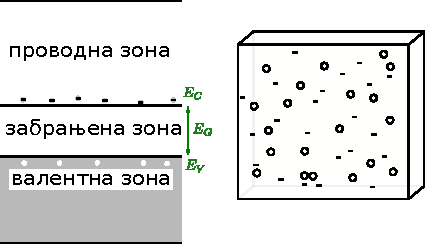
\includegraphics[width=0.6\linewidth]{Figures/diagram-energy-lvls.pdf}
	\caption{Дијаграм енергетских зона сопственог полупроводника. Постоји случајна расподела електрона и шупљине чије концентрације су једнаке.}
	\label{fig:diagram-energy-lvls}
\end{figure}

Односи су најједноставније представљени у виду дијаграма енергетских зона кристала. На слици \ref{fig:diagram-energy-lvls} је приказана схема дијаграма енергетских зона сопственог полупроводника. Електрони који формирају хемијске везе праве континуалну зону нивоа која се назива валентна зона. Изнад ње постоји енергетски процеп у коме не постоје дозвољени нивои у идеалном кристалу, а потом још једна зона нивоа која се назива проводна зона. Енергетски процеп $E_G$, представља енергију потребну да се електрон ослободи ковалентне везе. Сувишни или проводни електрони могу имати енергије у доњем делу проводне зоне. Најниже енергетско стање у зони $E_C$ одговара електрону који се не помера други виши нивои одговарају електронима који се крећу кроз кристал са додатном кинетичком енергијом. Шупљине одговарају стањима близу врха валентне зоне $E_V$ где недостају електрони. У сопственом полупроводнику, електрони и шупљине настају у једнаком броју термалном побудом електрона из валентне зоне у проводну зону, и имају случајну расподелу али их има исти број.

У полупроводнику \textit{n}-типа, као што је приказана на слици \ref{fig:n-p-type-diagram-energy-lvls} (а) постоји велики број електрона у проводној зони и веома мали број нула у валентној зони. Енергетски нивои, који одговарају електронима који се налазе у близини донорских примеса из групе V, су обично у енергетском процепу мало испод проводне зоне. Ово значи да мало енергије је потребно да се јонизује донор и електрон пребаци у проводну зону. Наелектрисање електрона у проводној зони је компензовано позитивним просторним набојем јона донора. Зона акцептора групе III (слика \ref{fig:n-p-type-diagram-energy-lvls}) се налазе мало изнад валентне зоне. Када код њих дођу електрони побуђени термалном енергијом из валентне зоне, постају негативно наелектрисани. Просторни набој шупљина је створен и компензован негативним акцепторским јонима. 

Заузетост зона је дата позицијом Фермијевог нивоа $E_F$. Вероватноћа $f$, да ниво енергије $E$ је заузет електроном је дата Ферми-Дираковом функцијом:

\begin{equation}
    f = \dfrac{1}{1+e^{\dfrac{E-E_f}{kT}} }
\end{equation}

\begin{info}
	Шта је Фермијев ниво?

	Највиши енергетски ниво који електрон може да заузме на апсолутној нули је познат као Фермијев ниво. Фермијев ниво лежи између валентне и проводне зоне зато што су нма апсолутној нули електрони на најнижем енергетском стању. Услед недовољне енергије на \SI{0}{\kelvin}, Фермијев ниво се може посматрати као море фермиона (или електрона) изнад ког електрони не могу да постоје. Фермијев ниво се мења како се материјали греју и како се електрони додају или одузимају из материјала. 

\end{info} % фермиони су исто поменути у дефиницији.

Енергетски процеп у полупроводнику је обично велики у односу на термалну енергију, $kT$ ($\approx 0.025$ е\SI{}{\volt} на собној температури), тако да се нивои изнад $E_F$ могу користити апроксимацију:

\begin{equation}
    f \approxeq e^{-\dfrac{E-E_f}{kT}}
\end{equation}

За нивое испод $E_F$ обично је лакше дати вероватноћу 

\begin{equation}
	f_p = 1-f = \dfrac{1}{1+e^{\dfrac{E_f-E}{kT}}}
\end{equation}

да је ниво незаузет, тј. да постоји шупљина. За нивое испод $E_F$,

\begin{equation}
    f_p \approxeq e^{-\dfrac{E-E_f}{kT}}
\end{equation}

Изрази за укупну концентрацију електрона и шупљина (број по запремини). означен \textit{n} и \textit{p} респективно, су у облику: 

\begin{equation}
	n = N_C e^{-\dfrac{E_C - E_F}{kT}}
\end{equation}

\begin{equation}
	p = N_V e^{-\dfrac{E_F - E_V}{kT}}
\end{equation}

где су $N_c$, $N_v$ споро мењају са температуром и односу на експоненцијалне факторе. Производ $np$ је независан од позиције Фермијевог нивоа и зависи само од температуре:

\begin{equation}
	n p = N_C e^{-\dfrac{E_C - E_F}{kT}} N_V e^{-\dfrac{E_F - E_V}{kT}} = N_C N_V e^{-\dfrac{E_C - E_V}{kT}} = N_C N_V e^{-\dfrac{E_G}{kT}}
\end{equation}

Овде $n$ је концентрација сопственог полупроводника код кога је $n = p$. Код полупроводника \textit{n}-типа, Фермијев ниво је изнад половине процепа, тако да је вредност $n$ фиксирана концентрацијом донорских тако да постоји електрична неутралност: 

\begin{equation}
	n - p = N^+_d
\end{equation}

\begin{figure}[ht!]
    \centering
	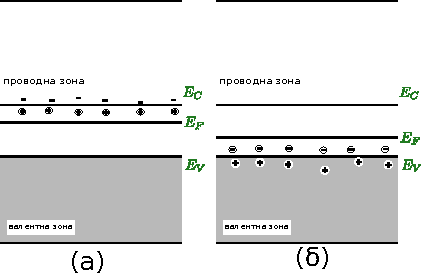
\includegraphics[width=0.6\linewidth]{Figures/metal-semiconductor-equi-diagram.pdf}
	\caption{Дијаграм енергетских зона полупроводника \textit{n} (а) и \textit{p} типа (б).}
	\label{fig:metal-semiconductor-equi-diagram}
\end{figure}

Концентрација мањинских носиоца, $p$ се повећава убрзано са температуром док се не достигне температура где су и $n$ и $p$ велики у односу на $N_d^+$ и проводност је у суштини сопствена. Сходно томе у полупроводнику \textit{p}-типа, у коме су акцепторски јони, $n$ и Фермијев ниво је испод центра процепа.

Фермијев ниво је еквивалентан хемијском потенцијалу електрона. Ако су два проводника повезана тако да се електрони могу пренети, релативни електростатички потенцијали ће бити подешени тако да су Фермијеви нивои два једнаки. Ако су материјали \textit{n}-типа  и \textit{p}-типа са слике \ref{fig:metal-semiconductor-equi-diagram} повезани, мали број електрона че бити пренет из \textit{n}-типа  у \textit{p}-тип. Тиме ће наелектрисати негативно \textit{p}-тип у односу на \textit{n}-тип и повећати електростатичку потенцијалну енергију електрона. Пренос електрона ће постојати док енергетски нивои материјала \textit{p}-типа не повећају у односу на \textit{n}-тип за толико да се Фермијеви нивои поклопе.

Количина примеса потребна за значајне промене у проводности германијума и силицијума су веома мале. Ово је дато на слици НЕМА, логаритамска скала, отпорност према $1/T$ за примерке германијума са различитим количинама антимона, донорске примесе. Ова карактеристика је на основу Пирсонових мерења од пре неколико година. Најчистији примерци доступни у то време су имале отпорност на собној температури од око 10\-20 \SI{}{\ohm\per\centi\meter}, што одговара $1$ донорском атому према $10^8$ атома германијума. Овај материјал (\textit{H.B.V.}) се користи за германијумске диоде које могу да издрже високе напоне у супротном смеру (\textit{High Back Voltage}) и такође код првих транзистора. Најчистији материјал доступан данас одговара $1$ донорском атому према $10^{10}$ прави велику разлику. Сви примерци на високим температурама прилазе сопственој линији која одговара чистом германијуму.

Проводни електрони и шупљине су веома покретни, и могу да се крећу кроз кристал за дужине од стотину или хиљаду међуатомских растојања, пре него што се расеју термалним кретањем или од нечистоћа или других несавршености. Ово би требало разумети са гледишта таласних особина електрона; талас може да се креће кроз савршено периодичну структуру без слабљења. У посматрању убрзања у електричним и магнетним пољима, таласна особина се може занемарити, и електрони и шупљине се посматрају као класичне честице са ефективном масу истог реда, али се разликују од обичне масе електрона. Ефективна маса је обично анизотропна, и разликује се за различите правце кретања у кристалу. Иста ефективна маса се може користити за термално кретање гаса електрона и шупљина. Средње термалне брзине су реда $10^7$ \SI{}{\centi\meter\per\second}.


\begin{info}
	Анизотропија је особина зависности од правца, и има супротно значење од изотропије која означава хомогеност у свим правца. Може се дефинисати и као разлика у физичкој особини неког материјала када се мери у различитим осама.
\end{info}

Расејање може бити описано појмом средњег слободног пута електрона и шупљина. У релативно чистим кристалима на собним температурама, расејање се дешава углавном због интеракција у термалним вибрацијама атома кристала. У мање чистим кристалима, или релативно чистим кристалима на ниским температурама, средњи слободни пут може бити одређен расејањем због атома нечистоћа. Због расејања, носиоци нису подједнако убрзани од стране електричног поља, већ имају просечну дрифт брзину пропорционалну пољу. Обично дрифт брзина је мања од просечне термалне брзине. Дрифт брзине могу бити изражене мобилностима електрона и шупљина.

За електрично поље $E$,

\begin{equation} % да се споје ове две формуле
	(V_d)_n = - \mu_n E
\end{equation}
\begin{equation}
	(V_d)_p = \mu_p E
\end{equation}

Због њиховог негативног наелектрисања, проводни електрони дрифтују у супротном смеру од поља. Величине за чист германијум на собној температури износе $\mu_n = 3800$ \SI{}{\centi\meter\squared\per\volt} и $\mu_n = 1800$ \SI{}{\centi\meter\squared\per\volt}. Ово значи да шупљине одржавају дрифт брзином \SI{1800}{\centi\meter\per\second} у пољу од \SI{1}{\volt\per\centi\meter}.

Изрази за проводност су:
\begin{itemize}
	\item \textit{n}-тип: $\sigma_n = n e \mu_n $
	\item \textit{p}-тип: $\sigma_p = p e \mu_p $
	\item сопствени: $\sigma = n e \mu_n  + p e \mu_p$
\end{itemize}

Није могуће одредити $n$ одвојено од мерења саме проводности. Постоји неколико начина да се одреди покретност; један од њих који је распрострањен је мерење Холовог коефицијента заједно са мерењем проводности. Као део истраживачког програма Бел Лабораторија, Пирсон и Хол су урадили мерења отпорности за широк опсег температура силицијума који садржи различите количине бора (акцептора из групе \rom{3}) и фосфора (донор из групе \rom{5}). Анализа ових резултата је дала додатну потврду теорији која је представљена. Слична мерења на германијуму су рађена у исто време од стране Ларк-Хоровица и његових колега, и још скорији комплетна мерења на оба материјала су урађена од стране других група. Резултат великог експерименталног и теоријског рада је потврда Вилсоновог модела у квантитативном погледу. 

% Овде Холов ефекат и Холов коефицијент као информација
\begin{info}
	Википедија - Холов ефекат је појава када у материјалу чврстог агрегатног стања кроз који је пропуштена струја и који је постављен у спољашње попречно магнетно поље, долази до појаве попречног напона. До појаве долази када је проводни материјал постављен тако да вектор магнетног поља заклапа прав угао са смером протицања електричне струје кроз проводник. Правац попречног напона који се јавља је управан и на правац магнетног поља и на правац протицања струје. Сила која ствара овај утицај је Лоренцова сила.
\end{info}

\begin{info}
	Википедија - Холов коефицијент је дефинисан као однос индукованог електричног поља и производа електричне густине и примењеног магнетног поља. То је особина материјала од кога је проводник направљен, пошто његова вредност зависи од типа, броја и особина носиоца наелектрисања које чине струју.
\end{info}

Носиоци се не крећу само под утицајем електричног поља, већ и дифузијом; дифузиона струја је пропорционална концентрационом градијенту. Изрази за концентрацију струја шупљина и електрона, су респективно:

\begin{equation}
	j_p = p \mu_p E - D_p grad p
\end{equation}

\begin{equation}
	j_n = n \mu_n E - D_n grad n
\end{equation}

% градијент је исто што и први диференцијал у простору

Ајнштајн је показао везу између мобилности и дифузионих коефицијената:

\begin{equation}
	\mu = D \dfrac{e}{kT}
\end{equation}

где је $k$ Болцманова константа. Дифузиона и кондукциона струја имају значајну улогу код транзистора.

\begin{figure}[ht!]
    \centering
	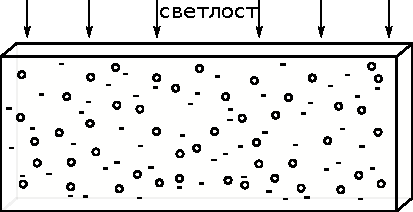
\includegraphics[width=0.6\linewidth]{Figures/diffusive-flow-light.pdf}
	\caption{Схематски дијаграм дифузионог тока електрона и шупљина створеног близу површине услед апсорпције светлости}
	\label{fig:diffusive-flow-light}
\end{figure}

Појам дифузије је први пут разматран од стане Вагнера у његовој теорији оксидације метала. Једначине су исцрпније анализиране у Френкеловој анализи дифузионог тока који се дешава када се осветли једна страна плоче, као што је приказано на слици \ref{fig:diffusive-flow-light}. Квант светлости подиже енергетски ниво електрона из валентне у проводну зону, стварајући проток електрона и шупљина у једнаком броју. Због рекомбинације проводних електрон -шупљина парова, концентрација опада како се дифузија дешава. Френкел је дао уопштене једначине тока када су електрони и шупљине присутне у покушају да урачуна Демберов ефекат (промена у контактним потенцијалима са светлошћу) и фото- магнетско- електрични (\textit{PME}) ефекат. Ово последње је аналогно са Холовим напоном кој се може видети измећу крајева плоче у трансверзалног магнетског поља (под правим углом у односу на папир из дијаграма). Претпоставка да је Демберов напон резултат разлике у мобилности, а тиме и дифузионих константи шупљина и електрона. За електричну неутралност потребно је да концентрације дакле и градијенти концентрације буду исти. Даље под условима мирне радне тачке ток електрона ка унутрашњости мора бити једнак току шупљина, тако да нема нето електричне струје. Ипак, ако је $D_n$ веће него $D_p$, дифузиона струја електрона би била већа него шупљина. Оно што се дешава је да настаје електрично поље $E$ које помаже шупљине и успорава електроне тако да изједначи струје. Интеграл $E$ даје разлику напона између површине и унутрашњости, што представља и промену у контактном потенцијалу. Као што ћемо представити касније, много веће промене у потенцијалу контакта од светлости могу доћи од ефеката површинских баријера.

\subsection{Исправљачки контакти}

% да ли је добар назив исправљачи?

Како би разумели како транзистор тачкастог споја ради, неопходно је знати неке од особина исправљачких контакта измећу метала и полупроводника. Уобичајени примери су бакар оксид и селен исправљачи и германијум и силицијум диоде тачкастог споја који проводе струју много лакше у једном смеру примењеног напона него у супротан. Пратићемо Шоткијеву слику, и користити као илустрацију спој полупроводника \textit{n}-типа. Слични аргументи се могу односити и на исправљаче \textit{p}-типа са одговарајућим променама у знаку потенцијала и наелектрисања. Најлакше је искористити енергетски дијаграм у коме су промене у енергетских зонама праве промене у електростатичком потенцијалу представљене дуж линије која је под правим углом са контактом, као на слици \ref{fig:n-p-type-diagram-energy-lvls}. Резултати исправљања од потенцијалне енергетске баријере на улазу које омета ток електрона преко контакта.

\begin{figure}[ht!]
    \centering
	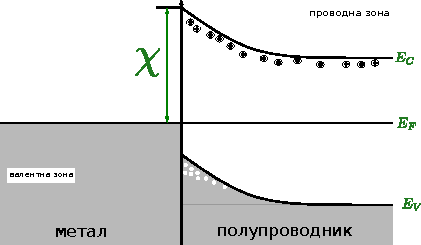
\includegraphics[width=0.6\linewidth]{Figures/n-p-type-diagram-energy-lvls.pdf}
	\caption{Равнотежа дијаграма енергетских нивоа за исправљачки спој метала и полупроводника дуж линије под правим углом у односу на спој. Варијације у енергетским зонама полупроводника стварају промене у електростатичком потенцијалу услед слоја некомпензованих непокретних наелектрисања. Укупна промена потенцијала од површине ка унутрашњости је таква да спушта Фермијев ниво у унутрашњости полупроводника у додир са нивоом код метала. У овом примери, постоји инверзија из \textit{n}-типа проводности у унутрашњости ка \textit{p}-типу на површини}
	\label{fig:n-p-type-diagram-energy-lvls}
\end{figure}

Фермијев ниво метала је близу највишем обично заузетим нивоима проводне зоне. Због природе интеракције метала и полупроводника, релативно велике енергије $\chi$, вероватно реда величине \SI{0.5}{\electronvolt}, која је потребна да се електрона из Фермијевог нивоа метала попне у проводну зону полупроводника. У унутрашњости полупроводника, који је електрично неутралан, позиција Фермијевог нивоа у односу на енергетске зоне које су одређене концентрацијом проводних електрона, дакле донора. У равнотежи, без примењеног напона, Фермијеви нивои метала и полупроводника су исти. Тако је због непокретних наелектрисања у близини метала у којима постоји варијација електростатичког потенцијала,  тиме и потенцијалне енергије електрона, као што је приказано на дијаграмима.
% регион баријере представља 

Унутар полупроводника постоји баланс између проводних електрона и позитивних донора. У региону баријере који је један од великих потенцијалних енергија за електроне, постоји неколико електрона у проводној зони. Некомпензована непокретна наелектрисања донора су избалансирана негативним наелектрисањем на самом споју. Ова наелектрисања, у ствари, прави потенцијалну баријеру. Ширина области просторног товара је обично реда $10^{-5}$ до $10^{-4}$ \SI{}{\centi\meter}.

% да ли је ово област просторног товара

Када се напон примени, већи део пада се дешава у области просторног товара. Правац лаког тока је такав у коме је полупроводник негативан у односу на метал. Зоне су подигнуте, баријера постаје ужа, и електрони могу лакше да се крећу из полупроводника у метал. У смеру високе отпорности, полупроводник је позитиван, зоне су спуштене релативно у односу на метал, и област се шири. Струја електрона која тече кроз метал је ограничена енергетском баријером $\chi$, која се мора премостити термалном побудом. 

Ако је $\chi$ довољно велико, Фермијев ниво на споју мора бити близу валентне зоне, подразумевајући инверзију из \textit{n}-типа проводности у унутрашњости у \textit{p}-тип у близини контакта. Област проводности шупљина, је названа, по Шоткију, област инверзије. Значајни део струје у контакту може бити у виду мањинских носиоца, у овом случају шупљина. Значајан резултат истраживачког програма у Бел Лабораторијама после рата је била истаћи значај ток мањинских носиоца.

\begin{figure}[ht!]
    \centering
	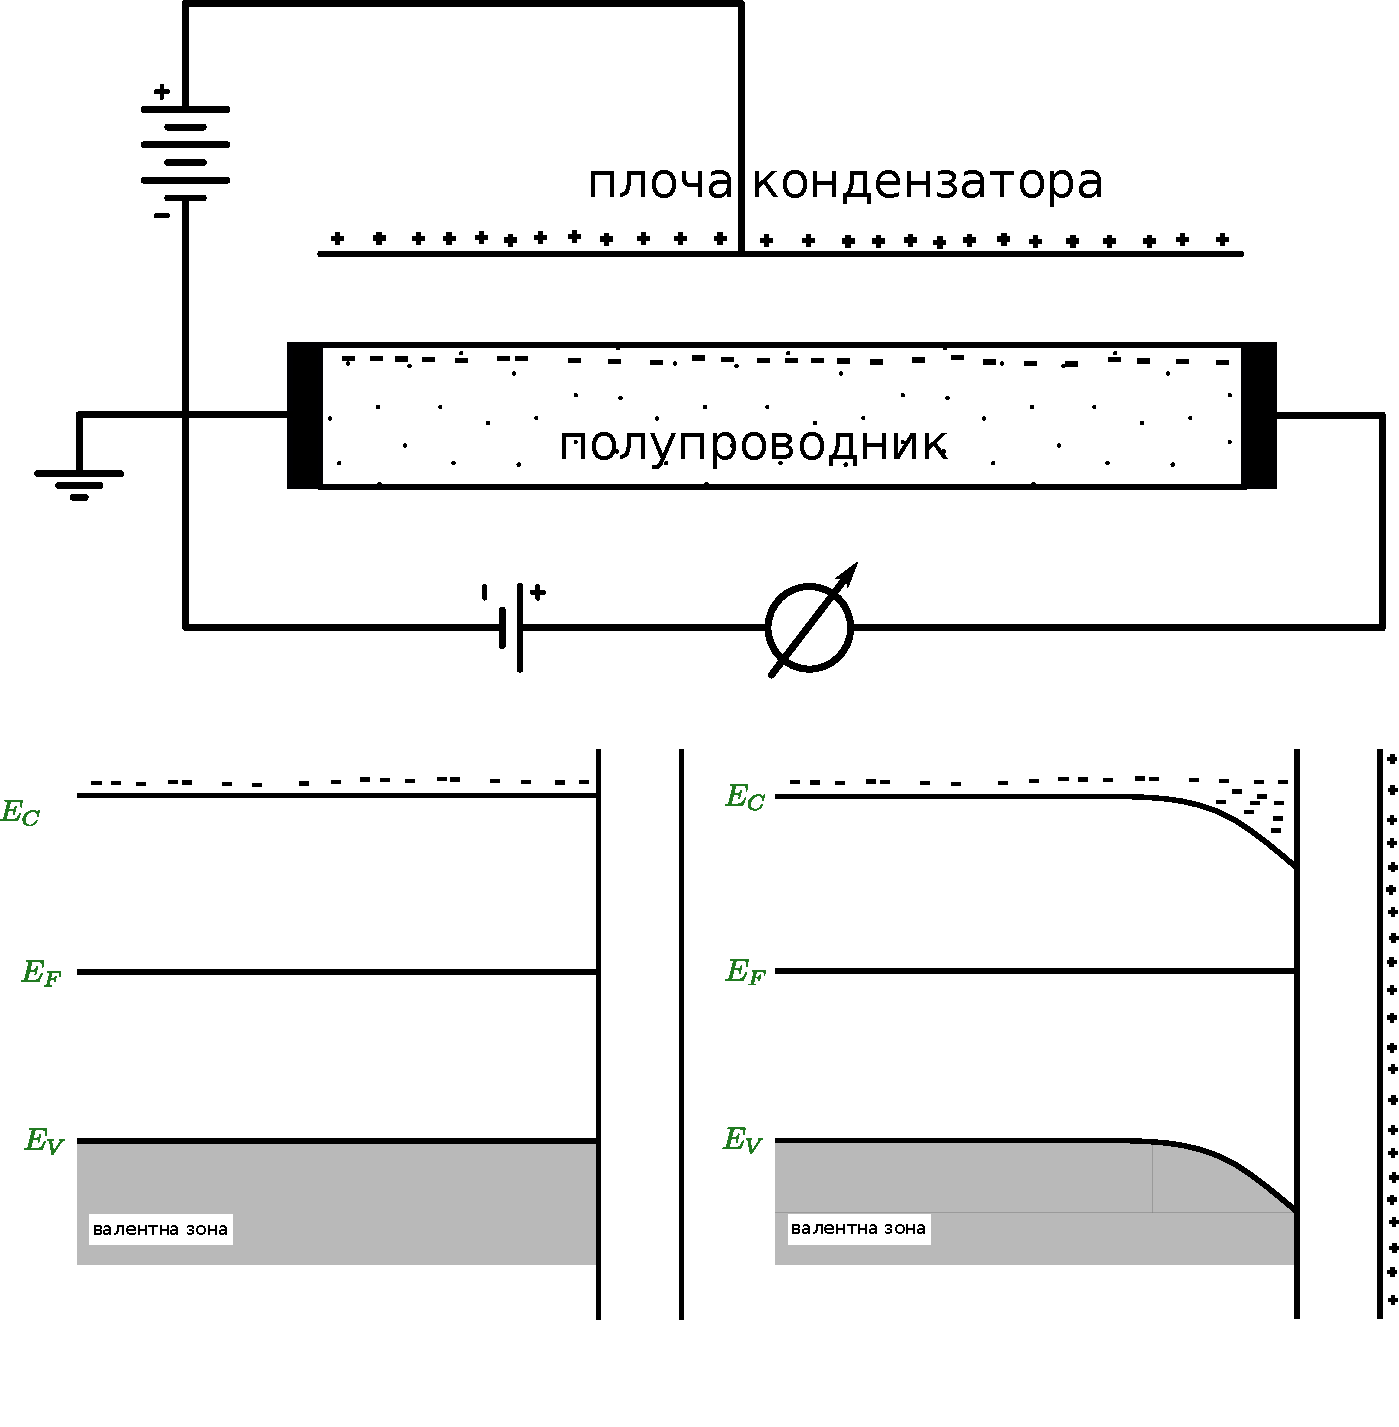
\includegraphics[width=0.6\linewidth]{Figures/field-effect-experiment.pdf}
	\caption{Схема дијаграма експеримента утицаја поља за полупроводник \textit{n}-типа без површинских стања}
	\label{fig:field-effect-experiment}
\end{figure}

\begin{figure}[ht!]
    \centering
	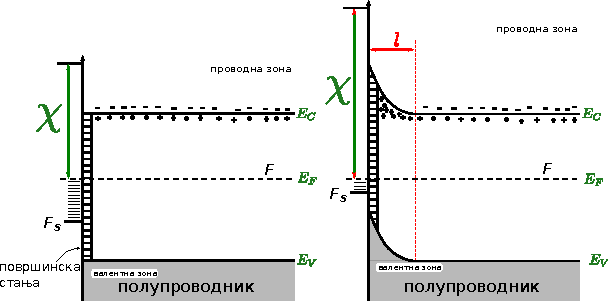
\includegraphics[width=\linewidth]{Figures/space-charge-barrier-formation.pdf}
	\caption{Стварање слоја баријере на слободној површи полупроводника}
	\label{fig:space-charge-barrier-formation}
\end{figure}

\subsection{Експерименти на тему површинских стања}

У уводу je поменуто да је негативни исход експеримента ефекта поља био важан фактор у претпоставци да постоје површинска стања на германијуму и силицијуму, и усмеравању истраживачког програма према студији површинских особина. Као што је приказано на слици \ref{fig:n-p-type-diagram-energy-lvls}, експеримент се састоји од прављења танког филма или плоче паралелно плочи кондензатора и мерење промене у проводности плоче са мењањем напона примењеног преко кондензатора. Хипотетички случај је приказан за полупроводник \textit{n}-типа без површинских стања. Када је поље плоче позитивно, негативно наелектрисање је индуковано на полупроводнику које се састоји од додатих електрона у проводној зони.
Количина индукованог наелектрисања је одређена примењеном напону и измереним капацитетом система. Ако је мобилност позната, очекивана промена у проводности се може одмах израчунати.

% шта значи evaporated film

% Да ли су силицијум и силикон исто?

Када су извођени експерименти на испареним филмовима германијума и силицијума, исходи су били негативни. У неким случајевима ефекат је био 1000 пута већи од експерименталне границе детекције. Анализа је назначила да велики део разликовања, можда и фактор до 50 или 100, долази од веома мале покретности електрона у филмовима у односу на дебљи материјал. Остатак је приписан штиту створеном од површинских стања.

Типова слојева баријера који могу постојати на слободној површини полупроводника \textit{n}-типа: (а) вишак проводности због инверзног слоја \textit{p}-типа (б) близу најмање површинске проводности (в) вишак проводности због акумулације области електрона.

Предвиђено је да ако површинска стања постоје, баријера која настаје на контакту са металом се може налазити и на површини полупроводника. Стварање оваквог слоја је илустрована на слици 	\ref{fig:space-charge-barrier-formation}. Заузетост површинских слојева је одређена позицијом Фермијевог нивоа на површини. На овој слици, претпоставка је да расподела површинских стања је таква да су стања сама по себи електрично неутрална ако се Фермијев ниво пресеца са позицијом $F_S$ релативно у односу на зоне. Ако не постоји површинска препрека,тако да се Фермијев ниво прелази површину изнад $F_S$, постоји вишак електрона и негативно наелектрисање на површини. Када је површина као цела неутрална, слој баријере је формиран ткао да се позитивно наелектрисање из унутрашњости компензује негативним наелектрисањем из површинских стања. Ако је густина површинских стања разумно велика, довољно негативно наелектрисања се може добити ако пресек Фермијевог нивоа пресеца само мало изнад $F_S$. 

Типови баријера који могу постојати на површини полупроводника \textit{n}-типа су приказани на слици ЏЏЏ. На левој страни (а) енергетски нивои су подигнути на површини како би валентна зона била ближа Фермијевом нивоу. Област инверзије обрнутог типа се формира, и постоји вишак проводности од мобилних шупљина у овом слоју. Негативно наелектрисање на површини је у равнотежи са наелектрисањем шупљина и непокретних донорских јона у области баријере. На делу слике (б) нивои су подигнути у близини површине али не довољно да формирају област баријере. Површинска отпорност је близу максимума. На делу слике (в) нивои су савијени на доле тако да створе акумулациону област вишка проводних електрона у близини површине. Наелектрисање на површини је сада позитивно и у равнотежи са негативним наелектрисањем слободних електрона у области.  

% postulated - suggest or assume the existence, fact, or truth of (something) as a basis for reasoning, discussion, or belief.
Претпостављено постојање површинских стања и површинских баријера на слободној површини германијума и силицијума одговорни су за неколико особина германијума и силицијума до дан данас загонетних. Они укључују:

\begin{itemize}
	\item мањак зависности исправљачких карактеристика у односу на радну фун металног контакта
	\item струја напон карактеристика на контакту направљен од два комада германијума
	\item чињенице да постоји слаб до никакав контакт разлике потенцијала између германијума \textit{n} и \textit{p} типа, као и силицијума \textit{n} и \textit{p} типа.
\end{itemize}

Док су доступни докази за површинска стања доста убедљиви, сви су посредне природе. Даље, ниједан од ових ефеката није дао било какак доказ за висину површинске баријере и расподеле површинских стања. Број напредних експеримената који могу дати конкретне доказе о површинским баријерама су предложени од Шоклија, Братена и Бардина. Шокли је предвидео да разлика у контактима бни била примећена код примерака \textit{n} и \textit{p} типа са великом концентрацијом примеса. Систематска студија Братена и Шоклија коришћењем силицијума и различитих количина донорских и акцепторских примеса се показала као истинита, и добијена је процена за концентрацију површинских стања. Још један експеримент је назначио присуство површинске баријере је мерење промене потенцијала контакта осветљивањем површине. Ово је само Демберов ефекат, за који је Френкел покуша да објасни разликом у мобилности електрона и шупљина генерисаних од светлости  и дифузијом унутрашњости. Пронађено је да је промена обично већа и често супротног знака него што је предвиђено Френкеловом теоријом која није узела у обзир површинску баријеру.

\begin{figure}[ht!]
    \centering
	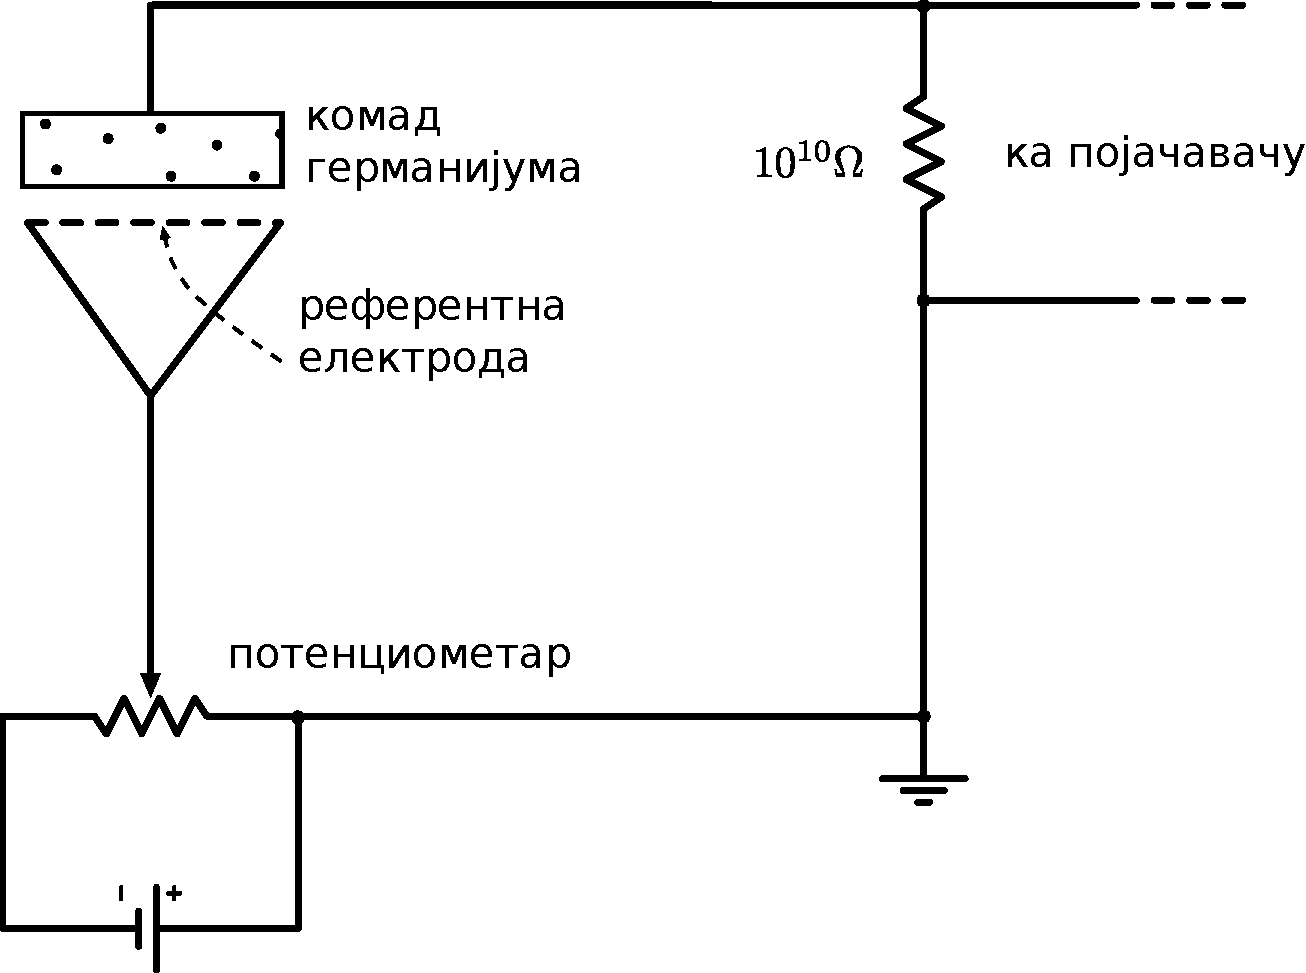
\includegraphics[width=0.7\linewidth]{Figures/sch-diagram-apparatus-measure-contact-potential.pdf}
	\caption{Схема дијаграм апаратус коришћена од стране Братена за мерење потенцијала контакта и промене потенцијала контакта под светлом}
	\label{fig:sch-diagram-apparatus-measure-contact-potential}
\end{figure}

Неки од тежих експеримената који су у том тренутку имали негативне исходе су извођени успешно много касније са побољшаним техникама, као што је описано од стране Братена у његовом говору. 

Апаратус који је користио Братен да измери потенцијал контакта и промене тог потенцијала услед светла су приказани на слици \ref{fig:sch-diagram-apparatus-measure-contact-potential}. Референтна електрода, обично од платине, је у виду паравана тако да пропушта светлост. Вибрирањем електроде, потенцијал контакта се може измерити Келвиновим методом. Ако се светлост која се пресеца на одговарајућој учестаности, пада на површину електроде и електрода је чврсто држана, промена у осветљењу се може измерити наизменичним напоном који настаје на кондензатору. Током ове студије, Братен је испробао неколико амбијенталних атмосфера и различитих температура. Приметио је велики ефекат када течни диелектрик попуни простор између електроде и полупроводничке површине. Он и Гибни су унели електролите и посматрали ефекте приписане великим променама површинске баријере са напоном преко електролита. Очигледно јони који се накупљају на површини стварају велико поље које пробија кроз површинска стања. 

\begin{figure}[ht!]
    \centering
	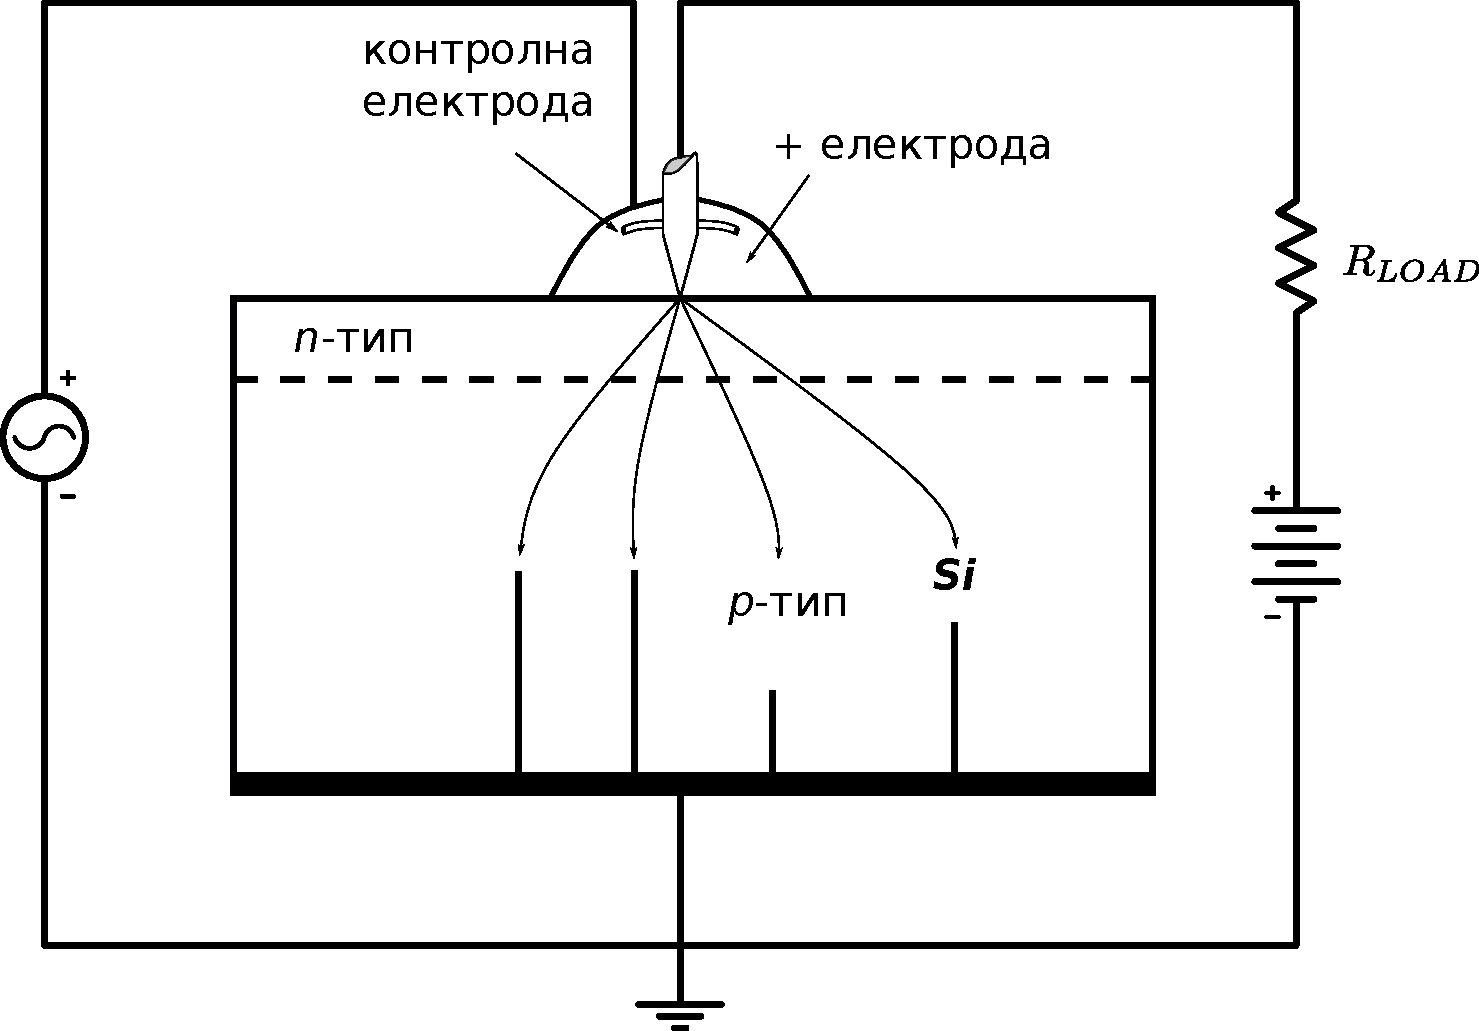
\includegraphics[width=0.7\linewidth]{Figures/observe-field-effect.pdf}
	\caption{Дијаграм експеримент у коме је посматран ефекат поља произведен од електролита у области инверзије проводности \textit{n}-типа на површини блока силикона \textit{p}-типа. Негативни потенцијал примењен на сонди у електролиту смањује број електрона у слоју инверзије и тако смањује струју електрона који теку ка тачкастом контакту који је обрнуто поларисан. Стрелице означавају конвенцијалан смер струје, електрони се крећу у супротном смеру. }
	\label{fig:observe-field-effect}
\end{figure}

\begin{info}
	Електролит је супстанца која може да ефикасно проводи струју кретањем јона, али не и кретањем електрона.
\end{info}

\begin{figure}[ht!]
    \centering
	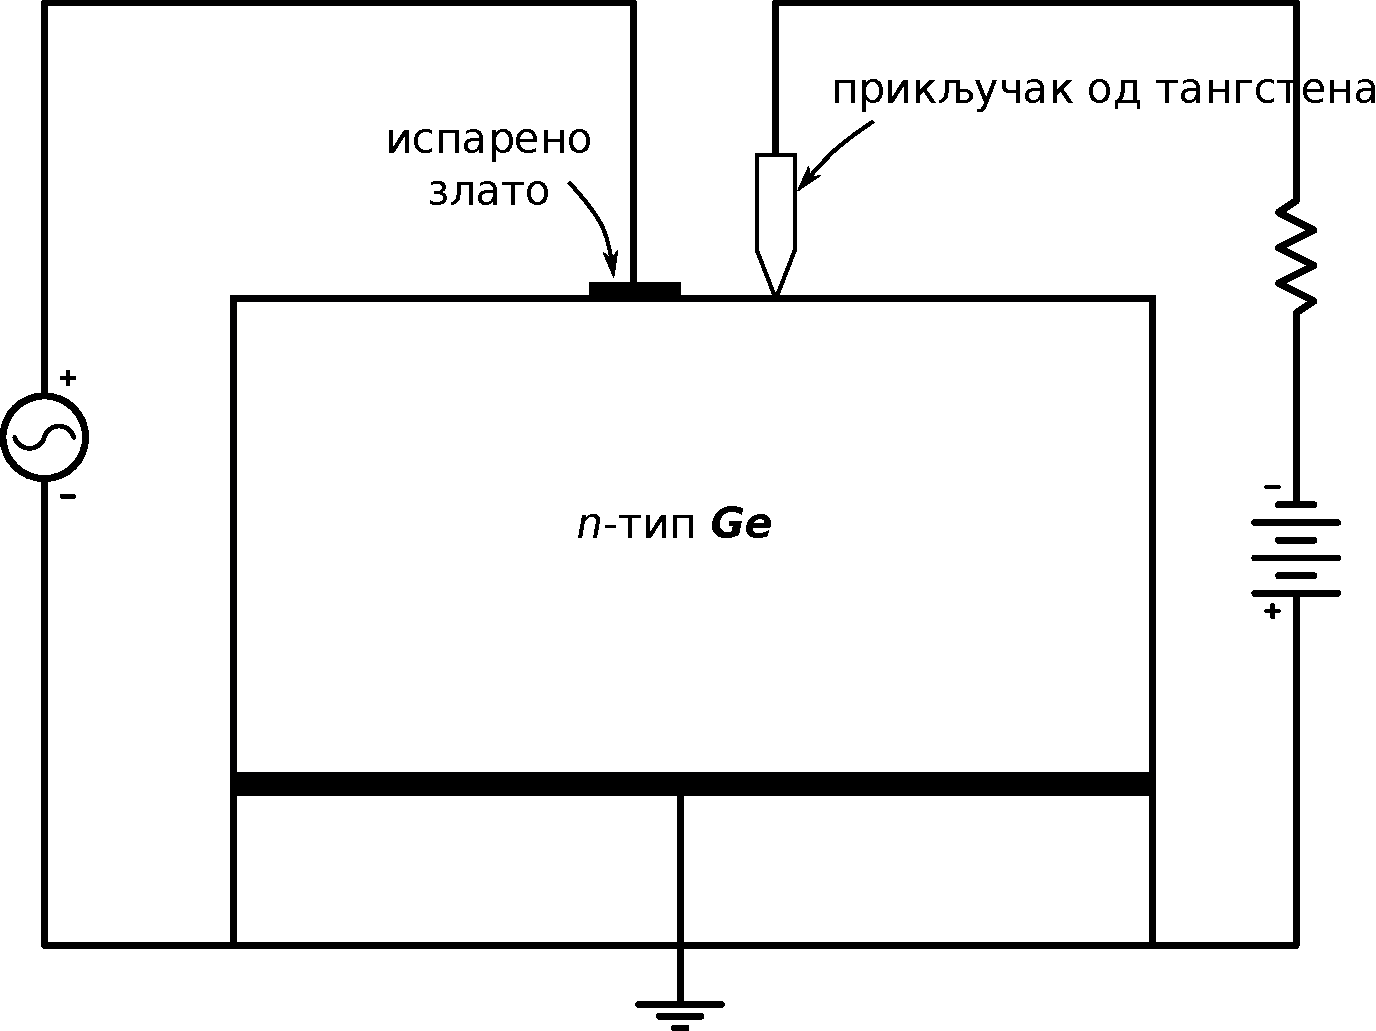
\includegraphics[width=0.7\linewidth]{Figures/observe-transistor-effect.pdf}
	\caption{Дијаграм експеримент у коме је посматран транзисторски ефекат. Позитивни напон примењен на златну тачку уноси шупљине у германијум \textit{n}-типа који пролазе кроз тачкасти контакт поларисан у обрнутом смеру- Пронађено је да повећање позитивног напона повећава \textit{reverse} струју. Када се повеже преко високе импедансе, промена напона тачкастог контакта је већа него промена на златном прикључку, оба измерена у односу на базу електроде}
	\label{fig:observe-transistor-effect}
\end{figure}

\textit{Експерименти у вези са областима инверзије}

Употреба електролита је омогућила метод мењања површинске баријере, тако да је могуће посматрати утицај поља у одговарајућем аранжману. Испаривани филм није коришћен због лоше структуре и слабе покретности. Техникама доступним у то време, било би тешко направити плочу од главног материјала довољно танко како би се приметио довољно јаки ефекат. Предложено је да би тај ефекат могао бити добијен на танком филму у главном материјалу посматрајући непосредно ток у слоју инверзије различитог типа проводности у близини површине. Ранији радови Ола и Шафа су назначили да је могуће добити слој инверзије \textit{n}-типа на силицијуму \textit{p}-типа, оксидацијом површине. Ако је направљен тачкасти контакт који исправља базу \textit{p} типа, за очекивати је да је контакт као слоју инверзије мале отпорности. 

Аранжман који је коришћен код Братена и Бардина у првобитним тестовима је приказан на слици \ref{fig:observe-field-effect}. Тачкасти контакт је окружен и изолован од капи електролита. Електрода у електролиту се могла користити да примени јако поље на површину полупроводника у близини контакта. Обрнуто, или смер високе отпорности у којој тачки је позитивна у односу на блок. Део повратне струје се састоји од електрона који теку кроз слој инверзије \textit{n}-типа ка контакту. Пронађено је да се величина ове струје може променити применом напона на електролитној сонди, и тако ефектом поља, се мења проводност инвертованог слоја. Пошто под статичним условима само слаба струја је текла кроз електролит, поставка се може користити као појачавач. Код првих тестова, појачање струје и снаге, али не и напона је примећено. Као што је предвиђено од очекиваног смањења у броју електрона у инвертованом слоју, откривено је да негативни напон примењен на сонду смањује јачину повратне струје ка контакту.

Потом је одлучено да се покуша слична поставка са блоком германијума \textit{n}-типа. Иако нисмо имали претходно знање о инверзији \textit{p-tipa} на површини експерименти су дефинитивно показали да се велики део повратне струје састоји од шупљина које се крећу у слоју инверзије у близини површине. Позитивно наелектрисање у напону на сонди је смањено повратном струјом. Значајно напонско као и струјно појачање и појачање снаге.

Због великих временских константи електролита који се користи, појачање постоји само за ниске учестаности. Покушали смо да заменимо електролите металном контролом електроде која је изолована од површини или слојем танког оксида или исправљачког контакта. Гибни је припремио површину анодизујући површину и потом испаравањем неколико златних мрља на њој. Иако ниједна није дала жељени контакт високе отпорности ка блоку, одлучено је да се посматрају добијени ефекти. Тачкасти контакт је постављен веома близу једне тачке и поларизован у обрнутом смеру (погледај слику \ref{fig:observe-transistor-effect}). Мали ефекат повратне струје је примећен када се тачка поларише позитивно, али у супротном смеру него што је примећено код електролита. Повећање позитивне поларизације је појачало а не ослабило повратну струју у тачкастом контакту. Ефекат је био довољно велики да да неко напонско појачање, али не и снаге. Овај експеримент је предложио да су се шупљине кретале у површину германијума из златне тачке, и да су убачене шупљине на овај начин се кретале у тачкасти контакт да појачају повратну струју. Ово је била прва назнака транзисторског ефекта.   

\begin{figure}[ht!]
    \centering
	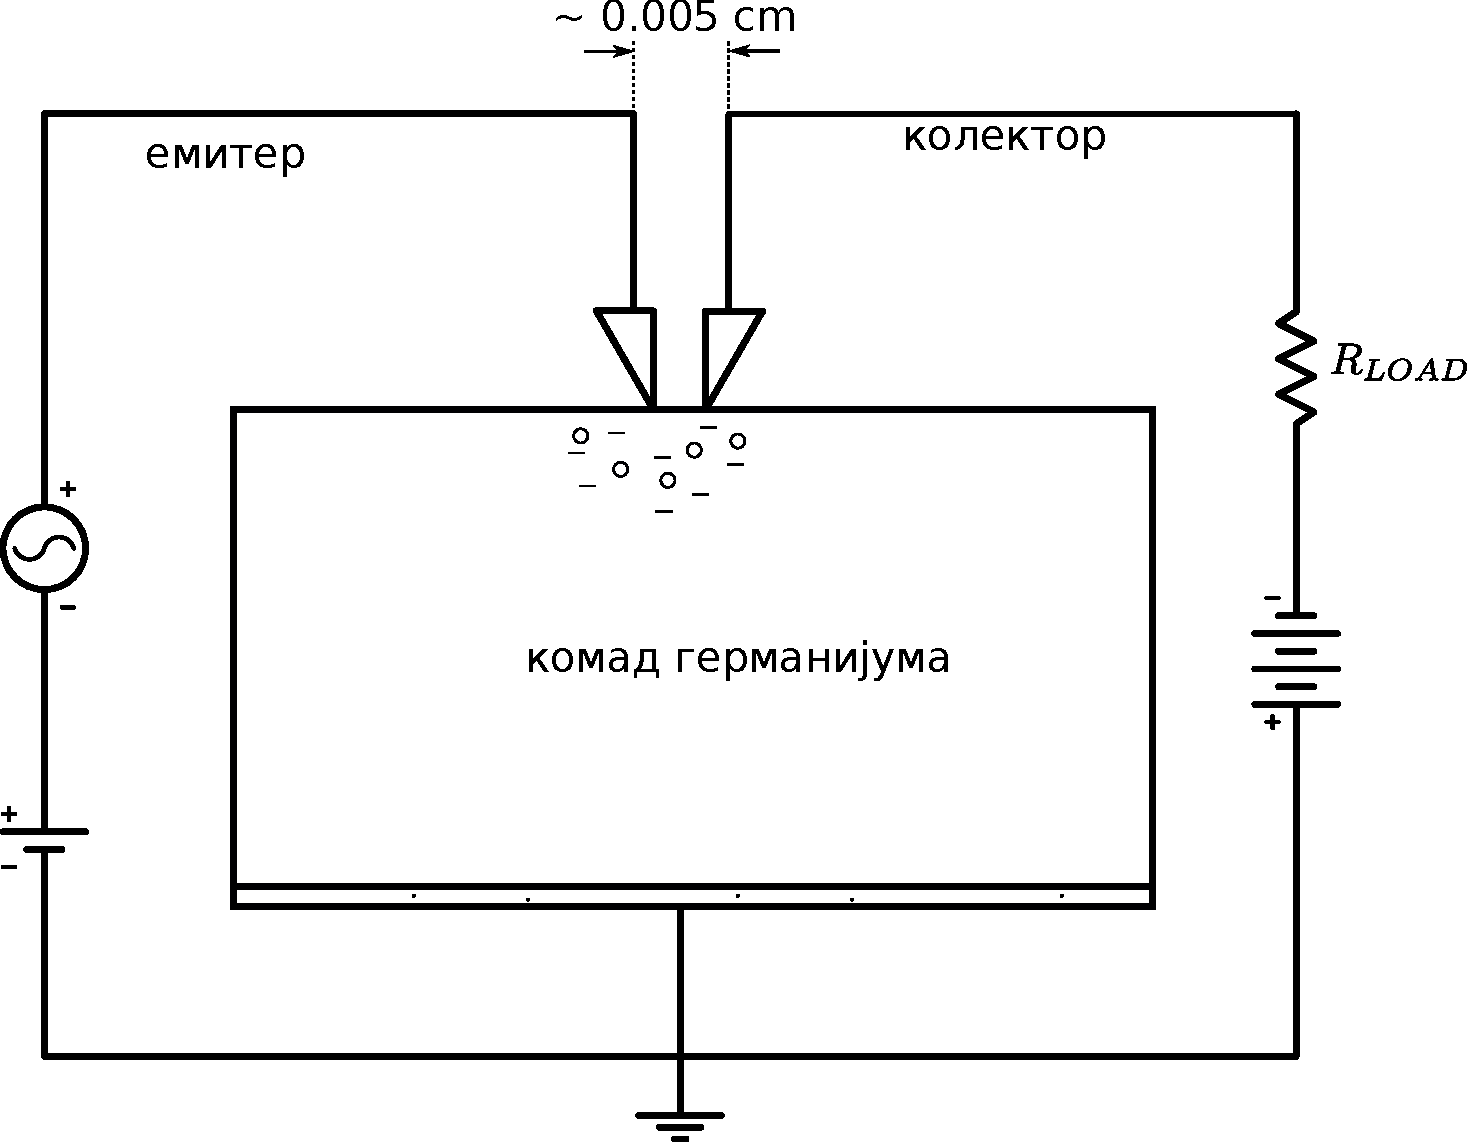
\includegraphics[width=0.7\linewidth]{Figures/schematic-point-contact-transistor.pdf}
	\caption{Схема транзистора тачкастог споја}
	\label{fig:schematic-point-contact-transistor}
\end{figure}

Предвиђено је да се може достићи појачање снаге ако се метални контакти на растојању реда \SI{0.005}{\centi\meter}. У првом покушају, који је био успешан, контакти су направљени од забоденог испариваног злата, и потом одвојеног злата на тачки клина помоћу оштрице направе два блиска контакта. После даље експериментације, показало се да је најлакши начин да се оствари жељено мало растојање, јесте да се користе два тачкаста контакта одговарајућег облика постављена један близу другог. Успех је остварен у првим покушајима, транзистор тачкастог контакта је створен. 

% Шта је испарено или испаривано злато?

Било је очигледно из експеримената да велики део и директне и повратне струје из германијумског тачкастог контакта је пренет мањинским носиоцима, у овом случају шупљинама. Да се ова чињеница препозната раније, транзистор је могао већ тада настати.

Понашање транзистора тачкастог контакта је приказано на слици \ref{fig:schematic-point-contact-transistor}. Када ради као појачавач, један од контакта - емитер, је поларисан \textit{d.c.} напоном у директном смеру, други колектор, у негативном или смеру високе отпорности. Трећи контакт, електрода базе ствара контакт ниске отпорности према блоку. Велики део директне струје се састоји од шупљина које улазе у блок. Струја из колектора се састоји делом од електрона који долазе из контакта и делом од шупљина које се крећу према контакту. Струја колектора ствара електрично поље у блоку које је у таквом смеру да привлачи шупљине унете на емитеру. Велики део емитерске струје, која улази под малом импедансом, тече у колекторском колу. Поларисан у обрнутом смеру, колектор има велику импедансу и може бити повезан са теретом високе импедансе. Дакле постоји велико напонско појачање улазног сигнала. Пронађено је да постоји и неко струјно појачање, дајући укупно појачање снаге од \SI{20}{\decibel} или више. Повећање струје шупљина на колектору утиче на баријеру на такав начина да појача струју електрона које тече из контакта.

Струја колектора мора бити довољно велика да произведе електрично поље и привуче шупљине ка емитеру. Оптимална импеданса колектора је значајно мања него она од обрнуто поларисане добре германијумске диоде. У првим експериментима, било је покушаја да се оствари ово третирањем површине тако да се створи велики слој инверзије проводности \textit{p}-типа на површини. У овом случају, велики део струје шупљина може да се креће у овом слоју инверзије. касније је откривено да бољи резултати могу да се остваре електричним стварањем колектора пуштањем великих струјних пулсева кроз њега. У том случају третман површине је мање критичан и већи део струје емитера тече кроз блок (\textit{bulk}).

Истраживања природе директних и повратних струја ка тачкастом контакту германијума ср рађена мерењем сонди мењањем потенцијала у близини контакта. Ова мерења су показала велика повећања у кондуктивности када је контакт поларисан у директном смеру и у неким случајевима доказе о постојању проводног слоја инверзије у близини површине која је поларисана у супротном смеру.

Пре него што је установљено да ли је корисна струја емитера ограничена само унутар слоја инверзије или може слободно да тече кроз блок, Шокли је предложио радикално другачији дизајн транзистора заснован на овој другој вероватноћи. Ово је транзистор споја где додати мањински носиоци из емитера се дифузијом крећу кроз танак слој базе ка колектору. Независно од овог предлога Шиве је направио транзистор тачкастог контакта у коме су емитер и колектор на супротним странама танке плоче германијума. Овако је дефинитивно показано да се убачени мањински носиоци могу кретати кроз мала растојања кроз блок материјала. Док транзистори се могу направити за рад на оба начина, дизајни који користе ток кроз блок материјала су се показали као најуспешнији. Спојни транзистори су надмашили транзисторе тачкастог контакта за већину примена.

После открића транзисторског ефекта, велики део истраживања код Бел Лабораторија је био посвећен студијама тока инјектованих мањинских носиоца у блоку материјала. Већи део ових истраживања је покренуто од Шоклија и биће описано од стране њега у наредном делу.

Истраживање површинских особина германијума и силицијума, заустављено неко време после 1948. због притиска осталих радова, је настављено од Братена и других, и сада је расцветано поље рада са импликацијама према одређеном броју научних поља осим полупроводничких, већ и области катализе и фотокондуктивности. Овај истраживачки програм ће бити описан од стране Братена.

Очигледно је да многе године истраживања великог броја људи, и пре и после открића транзисторског ефекта је било неопходно да донесе знање о полупроводницима његовом тренутном развоју...

%----------------------------------------------------------------------------------------
%	Shockley
%----------------------------------------------------------------------------------------

\section{Транзисторска технологија побуђује нову физику - Шоклијев лауреат}

Превод Шоклијевог предавања коришћеног за нобелову награду, предавање на пријему Нобелове награде, 11. децембар 1956.

\subsection{Увод}

Циљ проналаска корисних уређаја иам јак утицај на избор истраживачких тема са којима сам ја повезиван. Често се каже да поседовање колико толико специфичног практичног циља може деградирати квалитет истраживања. Ја не верујем строго да је то случај и како бих доказао у овом предавању одабрао сам пар примера физике полупроводника из истраживачких пројеката који су дефинитивно мотивисани практичним разматрањима.

Важни део индустрије САД се слаже са идејом да је истраживање основа значајно из практичних разлога. Ово је изразито случај са Бел Телефон Лабораторијама (\textit{eng. Bell Telephone Laboratories})где моји сарадници и ја, такође са још много колега, радимо на пројектима описаним у овим предавањима. Однос Бел Телефон Лабораторија је несумњиво резултирао у значајном уделу због гледишта 4 човека који су били његови истраживачки директори и потом његови председници. Сваки од ових људи, Х. Д. Арнолд, Ф. Б. Џуит, О. Е. Бакли и М. Џ. Кели, је такође био активан и успешан у управним и цивилним пословима. Сви су добили детаљну индоктринацију у истраживачким гледиштима за време њиховог докторантског тренинга у физици. Мој лични контакт са двојицом од ових људи је имао значајан утицај на планирање полупроводничких истраживачких програма како ћу их касније поменути.

Моја одлука да дођем у Бел Телефон Лабораторије одмах по завршетку докторских студија 1936. је била под значајним утицај чињеница да би ми супервизор био Ц. Џ. Дејвисон. Након мог доласка додељен ми је доктор М. Џ. Кели за докторантски програм на тему електронских цеви (\textit{eng. vacuum tubes}). За време ових студија Др Кели је причао са мном о његовима идеалима о вршењу свих телефонских прекидача електронски уместо металних контаката. Иако Ја нисам одабрао да наставим рад на електронским цевима и добио слободу да се бавим основним истраживачким проблемима у физици полупроводника, разговор са др Келијем ме је оставио у константном опрезу за могуће примене полупроводничких ефеката за решавање проблема у телефонским централама. До сада мој допринос транзисторској електроници, инспирисан даном потпуно електронске телефонске централе, је био значајно погуран мојим искуствима за време раних година у Лабораторијама.

Пре напуштања теме о истраживању у индустрији, волео бих да изразима своја гледишта о речима које се често користе за класификацију истраживања у физици: нпр. чиста, примењена, неограничена, фундаментална, основна, академска, индустријска. практична, итд. Чини се да веома често неке од ових речи се користе у негативном контексту, с' једне стране како би се умањили практични циљеви проналаска нечег корисног, са друге стране како би се одбацила могућа дугорочна вредност ових залажења у нове области где се корисни исходи не могу предвидети.  Често ме питају да ли је експеримент који сам испланирао за чисто или примењено истраживање; мени је важније да знам да ли ће експеримент донети ново и одрживо знање о природи ствари. Да ли је вероватно да ће изродити такво знање, то је, по мом мишљењу, добро фундаментално истраживање; и ово је далеко значајније од тода да ли је моје мотивација чисто естетска сатисфакција онога ко врши експеримент са једне стране или напредак и стабилност транзистора велике снаге са друге стране. Биће потребна оба типа како би се допринео највећи допринос човечанству, како је тражено у Нобеловом тестаменту.

\subsection{Пет основних несавршенства}

Пре него што почнемо расправу од одабраним експериментима у транзисторској физици, желим да се надовежем даље на др Бардинове напомене о карактеристикама и интеракцијама електрона, шупљина, донора и акцептора. Зарад бољег појашњења предложићу и аналогију са воденим растворима киселина, база и соли као помоћ у излагању.

Дисоцијација чисте воде у позитивне јоне хидрогена и негативне хидроксилне јоне задовољава закон о дејству маса (Гулдберг-Вагеов закон из хемије):

\begin{equation}
    [H^+] [OH^-] = f(T)
\end{equation}

где је концентрација $H_2O$ скоро константа за благе растворе где се може претпоставити за константу а не експлицитно. Аналогно овој једначини 

\begin{equation}
    p n = f(T)
\end{equation}

за полупроводник где је \textit{n} и \textit{p} концентрација електрона и шупљина. Једначина је тачна, ако ни n ни p нису толико велики да се њихова статистика дегенерише (?). Нормално веза електронски пар овде игра улогу нераздвојени молекул воде. У чистој дејонизованој води и у чистом полупроводнику, електрична неутралност захтева да концентрација позитивних наелектрисања буде једнака негативном наелектрисања:

\begin{multicols}{2}
    \begin{equation}
        [H^+] = [OH^-]
    \end{equation}\break
    \begin{equation}
        p = n
    \end{equation}
\end{multicols}
  
Полупроводник који је толико чист, да његове нечистоће се могу занемарити се назива сопствени полупроводник. (\textit{intrinsic}) Користећи потписани знак $i$ kao назнаку, у том случају имамо:

\begin{multicols}{2}
    \begin{equation}
        p_i = n_i
    \end{equation}\break
    \begin{equation}
        n_i^2= f(T)
    \end{equation}
\end{multicols}

Концентрација $n_i$ се назива сопствена концентрација.
Хемијска аналогија $n$ типу полупроводника је база и њена електронска неутралност једначина је:

\begin{multicols}{2}
    \begin{equation}
        [H^+] + [Na^+] = [OH^-]
    \end{equation}\break
    \begin{equation}
        p + N_d = n
    \end{equation}
\end{multicols}

где је $N_d$ концентрација донора и претпоставка је да су сви донори потпуно јонизовани.

Слично је и за $p$ -тип полупроводника где је аналогија киселина:

\begin{multicols}{2}
    \begin{equation}
        [H^+] = [OH^-] + [Cl^-]
    \end{equation}\break
    \begin{equation}
        p = n + N_a
    \end{equation}
\end{multicols}

где је $N_a$ концентрација акцептора.

Неутрална со такође има свој пандан која се назива компензовани полупроводник. У овом случају концентрација донора и акцептора је једнака тако да имамо електричну неутралност:

\begin{equation}
    p + N_d = n + N_a
\end{equation}

се сведе на једнакост $n$ и $p$ тако да је свака једнака $n_i$. Електрична проводност савршено компензованог кристалa силицијума или германијума је скоро једнака оној од сопственог кристала; могу постојати мале разлике услед смањења покретности расипањем наелектрисаних јона. Разлика између мале проводности савршено компензованог полупроводника и велике проводности неутралног раствора соли лежи у чињеници да су донори и акцептори закопани у месту у полупроводнику (у кристалној решеци), док су катјони и анјони соли имају покретност поредиву са $OH$ јоном. Компензација, или превелика компензација, игра кључну улогу у производњи полупроводничких уређаја. Нпр. дозвољава конверзију $n$ тип материјала у $p$-тип додавањем акцепторских примеса без потребе за одузимањем донора. Кристал прављен од $n$-типа се може променити само додавањем вишка акцептора.

Речи већина и мањина се често користе у дискусији о полупроводницима. У $n$ -типу полупроводника, већински носиоци су електрони, а мањински шупљине.

Шупљине, електрони, донори и акцептори представљају 4 од 5 врста несавршености који се морају узимати у обзор како би разумели полупроводничке ефекте. Петој несавршености је дат назив \textit{deathnium}. Хемијска аналогија за \textit{deathnium} је катализатор. У случају воде као пандана кристалу, колико ја знам, не постоји одговарајући катализатор од значаја. Оно што \textit{deathnium} ради је убрзава остваривања еквилибријума између шупљина и електрона. Ако због различитих могућих поремећаја од значаја у транзисторској електроници, концентрација мањинских носиоца је нпр. значајно повећани, онда ће се мањински носиоци рекомбиновати са већинском носиоцима правећи везе електронских парова, и на овај начин успоставити еквилибријум. \textit{Deathnium} катализује процес рекомбинације. Симболи за 5 несавршенства полупроводника су приказани у табели \ref{table:imperfections-symbols}.


\begin{table}[ht]
	\centering
	\begin{tabular}{|c|l|}
		\hline
		- & (слободни) електрони \\
		\hline
		+ & шупљина\\ 
		\hline
		$\square$ & \textit{Deathnium} \\ 
		\hline
        $\oplus$ & донор\\ 
		\hline
		$\ominus$ & акцептор \\ 
		\hline
        
	\end{tabular}
	\caption{Симболи за несавршенства} 
    \label{table:imperfections-symbols}
\end{table}

Улога \textit{deathnium}-a се може илустровати као феномен фотокондуктивности. Ако осветлимо германијумски кристал, онда ће парови електрона и шупљина тако формирани пренети кондуктивност на кристал. Таква кондуктивност се назива и фотокондуктивност. Ако се извор светлости уклони, фотокондуктивност ће одумрети, услед рекомбинације шупљина и електрона. Дакле, ако електрон упаде у непотпуну везу, један шупљина-електрон пар ће бити елиминисан. 

\begin{info}
    Извор википедија - За несавршенство \textit{Deathnium} се испоставило да најчешће представља трагове бакра у полупроводнику првих биполарних транзистора (настају услед контаминације производних полигона) који је узроковао дубоке замке скраћујући животни век транзистора. Новије технологије су успеле да га заобиђу.
\end{info}

\begin{info}
	Извор википедија - Замке дубоког нивоа или дефекти дубоког нивоа су генерално нежељени типови електронских поремећаја у полупроводницима. Они су "дубоки" у смислу да енергија потребна да се уклони електрон или шупљина из те замке у валентни или проводни енергетски опсег је много веће од карактеристичне термалне енергије $kT$, где је $k$ Болцманова константа, а $T$ температура. Дубоке замке ометају корисне типове примеса компензујући типове већинских носиоца, уништавајући или слободне електроне или шупљине у зависности који су чешћи. Такође ометају и рад транзистора, светлећих диода као и електронски и оптоелектронских направа, додавајући међупростор унутар енергетског процепа (\textit{bandgap}). Дубоке замке скраћују нерадијативни животни век носиоца и кроза Шокли-Рид-Хол процес организују рекомбинацију мањинских носиоца имајући штетан ефекат на дејство полупроводничког уређаја. Тако дубоке замке нису повољне у многим оптоелектронским уређајима како могу довести до лоше ефикасности и великог кашњења у одзиву.

	Чести хемијски елементи који праве дубоке дефекте у силикону укључују гвожђе, никл, бакар, злато и сребро. Уопштено прелазни метали стварају овај ефекат, док лаки метали као алуминијум не.

	Површинска стања и кристалографски поремећају у кристалној решеци такође играју улогу дубоких замки. 
\end{info}

% Шокли-Рид-Хол процес ? Зашто лаки метали нису штетни?

Да је процес рекомбинације шупљина и електрона директан, животни век би био исти за све германијумске кристале. Експерименти, ипак показују да веома слични германијумски кристали могу имати животне векове који се разликују и до 1000 пута. У једном кристалу, животни век може бити милисекунда, док у другом може бити микросекунда. Ова варијација у животном веку значи да постоји нека несавршеност која катализује рекомбинацију шупљина и електрона. 

У ствари, постоје различити типови \textit{deathnium}-a. Нпр. ако електрони имају енергију од неколико милиона електрон волти (eV) на германијумском кристалу, животни век је додатно скраћен. Истраживање са Пардју Универзитета је показало да такво бомбардовање прави поремећај међу атомима германијума. Електрон са великом енергијом може да избаци германијумски атом са своје позиције у кристалној структури, стварајући празнину тамо где је био атом, узрокујући да избачени атом постане или вишак или да се нађе у међупростору - тамо где иначе не би постојао атом. Откривено је на Бел Телефон Лабораторијама да реметилачки ефекти играју улогу \textit{deathnium}-a. Пронађено је и да нечистоће бакра и никла у германијуму узрокују означена скраћења животног века.

Рекомбинациони центар (\textit{deathnium}) хвата наизменично електрон и шупљину и тако катализује њихову рекомбинацију. Када ухвати електрон постаје замка за шупљину. Пошто је карактеристика за све микроскопске процесе да иду и уназад као и у напред. Термално активирани процес генерације шупљине и електрона је такође  могуће да се деси у \textit{deathnium}-у. Под условом термалног еквилибријума, и процес рекомбинације и генерације се дешава константно.  Енергија потребна да се генерише пар шупљина-електрон се добија од термалне енергије вибрације атома у германијумском кристалу. услов за термални еквилибријум када оба процеса се изједначе. Германијум на собној температури има кондуктивност \SI{0.02}{\per\ohm\per\cm}.
Пошто концентрација шупљина и електрона па закону дејства маса, производ $n$ и $p$ не зависи од концентрације \textit{deathnium}-а. Нпр. ако дуплирамо концентрацију \textit{deathnium}-а, дуплираћемо и брзину рекомбинације и генерације, али ће еквилибријум шупљина и електрона остати непромењен. Докази да су механизми \textit{deathnium}-а тачни је добијено посматрањем зависности брзине рекомбинације у односу на густине електрона и шупљина.


\subsection{Ефекат електричног поља}

Експеримент који је одиграо највећу улогу у побуђивању програма транзисторске електронике у Бел Телефон Лабораторијама је био такозвани експеримент ефекта поља. Ја сам направио овај експеримент као директни резултат покушаја проналаска полупроводничког појачавача који има различите улазна и излазна кола. Од тада познатих особина полупроводника, закључио сам да танки слој силикона или германијума би имао значајну промену у својој проводности ако би од њих направио један пар кондензаторских плоча и кондензатор је јако напуњен. Површинско наелектрисање, представљено као промена у покретним носиоцима, би могло да повећа или смањи проводност танког филма.

Одређени број експеримента је иницијално покушан користећи испарене слојеве и друге танке слојеве. Ово је све дало занемарљиве ефекте и напредак није постојао док Бардин није предложио своју теорију о површинским стањима да објасне недостатак видљивог ефекта. Бардинов модел је објаснио неколико претходно непознатих феномена који су довели до предлога да експеримент утицај поља на течност-ваздух температури како би укопали површинска стања. Ово је дало први позитиван исход. Како је ово довело до низа експеримената кулминирајући у \textit{point-contact} транзистору који је објашњен у Бардиновом предавању.

Први рад позитивног ефекта је направљен од стране Г. Л. Пирсона као аутора 1948 године. Тренутно експеримент утицаја поља игра веома битну улогу у мерењу особина полупроводничких површина. Са практичне стране утицај поља се може користити за прављење транзисторских појачавача који имају интересантне особина - веома различите од  \textit{junction} транзистора. 

\subsection{Инјекција и дрифт}

У тренутку проналаска \textit{point-contact} транзистора од стране Бардина и Братаина постојао је велики број неразрешених питања у вези са његовим режимом рада. Оригинални транзистор је показао доказе о спрезању (?) између улаза или емитерске тачке и излаза или колекторске тачке кроз проводност у танком површинском слоју који је супротног типа од базног материјала који лежи испод. Нешто касније је настала идеја да емитер можда инјектује мањинске носиоце у тело полупроводника. Развој идеје је дошао од две независна догађаја: проналаска \textit{junction} транзисторске структуре од присутног аутора (као што  смо напоменули испод, инјекција игра кључну улогу у \textit{junction} транзистору) и запажању Ј. Н Шајва да транзисторско дејство се може догодити на тачкама са супротних страна танке плоче полупроводника.

\begin{figure}[ht!]
    \centering
	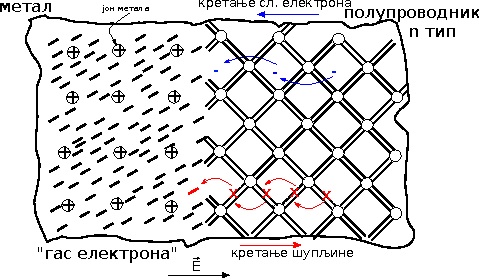
\includegraphics[width=0.8\linewidth]{Figures/metal-semiconductor-junction.pdf}
	\caption{Два могућа механизма за струју близу емитерске тачке}
	\label{fig:electron-hole-motion}
\end{figure}

Како би тестирали модел инјекције носиоца Џ. Р. Хејнс и аутор су сарађивали на експерименту дрифт-покретност или Хејнсов експеримент на германијумским примерцима. Како би разумели значај експеримента
у разјашњавању рада транзистора механизам у струјном току на метал полупроводник контакту мора бити разматран.

На Сл. \ref{fig:electron-hole-motion} метал је приказан у сликовној моди. Валентни електрони у металу се посматрају као гас електрона, који прожима целу структуру. Дакле електрони нису заробљени унутар валентних веза као што је случај код изолатора. Електронски гас може да се креће слободно кроз структуру метала, и ова чињеница одговара за високу кондуктивност метала. У горњем делу Сл. \ref{fig:electron-hole-motion} један од процеса за уклањање електрона из полупроводника је представљен. Пошто је полупроводник н типа, има вишак електрона, ови слободни електрони могу бити привучени металу од његовог позитивног наелектрисања и онда уђу у метал како би произвели струју електрона који теку из емитерског прикључка кроз прикључни вод.

Још један могуће механизам за пренос електрона из полупроводника у метал је приказан у доњем делу Сл. \ref{fig:electron-hole-motion}. У овом случају, електрон се повлачи из једне од валентних веза  близу метала. Овај процес такође привлачи електрон из полупроводника, али када се пренос догоди, шупљина остаје у полупроводнику. Шупљина бива одбијена од стране позитивног наелектрисања са стране емитерског прикључка и помера се све дубље у полупроводник. Оба процеса представљена имају исти ефекат барем што се тиче метала повезаног на емитер и прикључног вода ка емитеру. Онда је очигледно да суптилнији експеримент од простог мерења струје кроз емитер је потребно како би показали оба процеса уклањања електрона из полупроводника. Подобни експерименти су планирани и изведени. као резултат је добијено да је могуће видети оба процеса приказана на Сл. \ref{fig:electron-hole-motion} и показати њихов удео у струји емитера. У ствари, код доброг емитера показано је да више од 90\% струје настаје од процеса који инјектује шупљине у полупроводник, док мање од 10\% од процеса који узима електроне.

У идеалном емитеру, целокупна струје би требало да настаје услед инјекције шупљина. Разлог за ово је да узимање електрона не ремети стање унутар полупроводника. Ако се електрони уклањају из полупроводника у близини емитера, они се  убрзано замењују електронима који теку из којег год прикључка којим затварамо коло. Код инјекција шупљина, ситуација ја потпуно другачија. Нормално, број шупљина а полупроводнику $n$ типа је занемарљива барем што се тиче утицаја на проводност. Ипак, када уклонимо електроне из валентних веза и инјектујемо шупљине, релативно велики број шупљина настане. Проводност полупроводника је повећана у околини емиторског прикључка, на начин као кад би осветлили полупроводник и стварали шупљина електрон парове. Овај поремећај у електронској структури се може користити за појачавачко дејство транзистора.

Уместо расправи о квантитативном експерименту, који је коришћен за разликовање између два процеса приказаних на Сл. \ref{fig:electron-hole-motion}, ја ћу објаснити квалитативни експеримент који показује да се инјекција шупљина стварно дешава на емитерском прикључку. Овај експеримент дозвољава квантитативна истраживања о понашању шупљина и показује метод директног мерења дифузије и дрифта.


\begin{figure}[ht!]
    \centering
	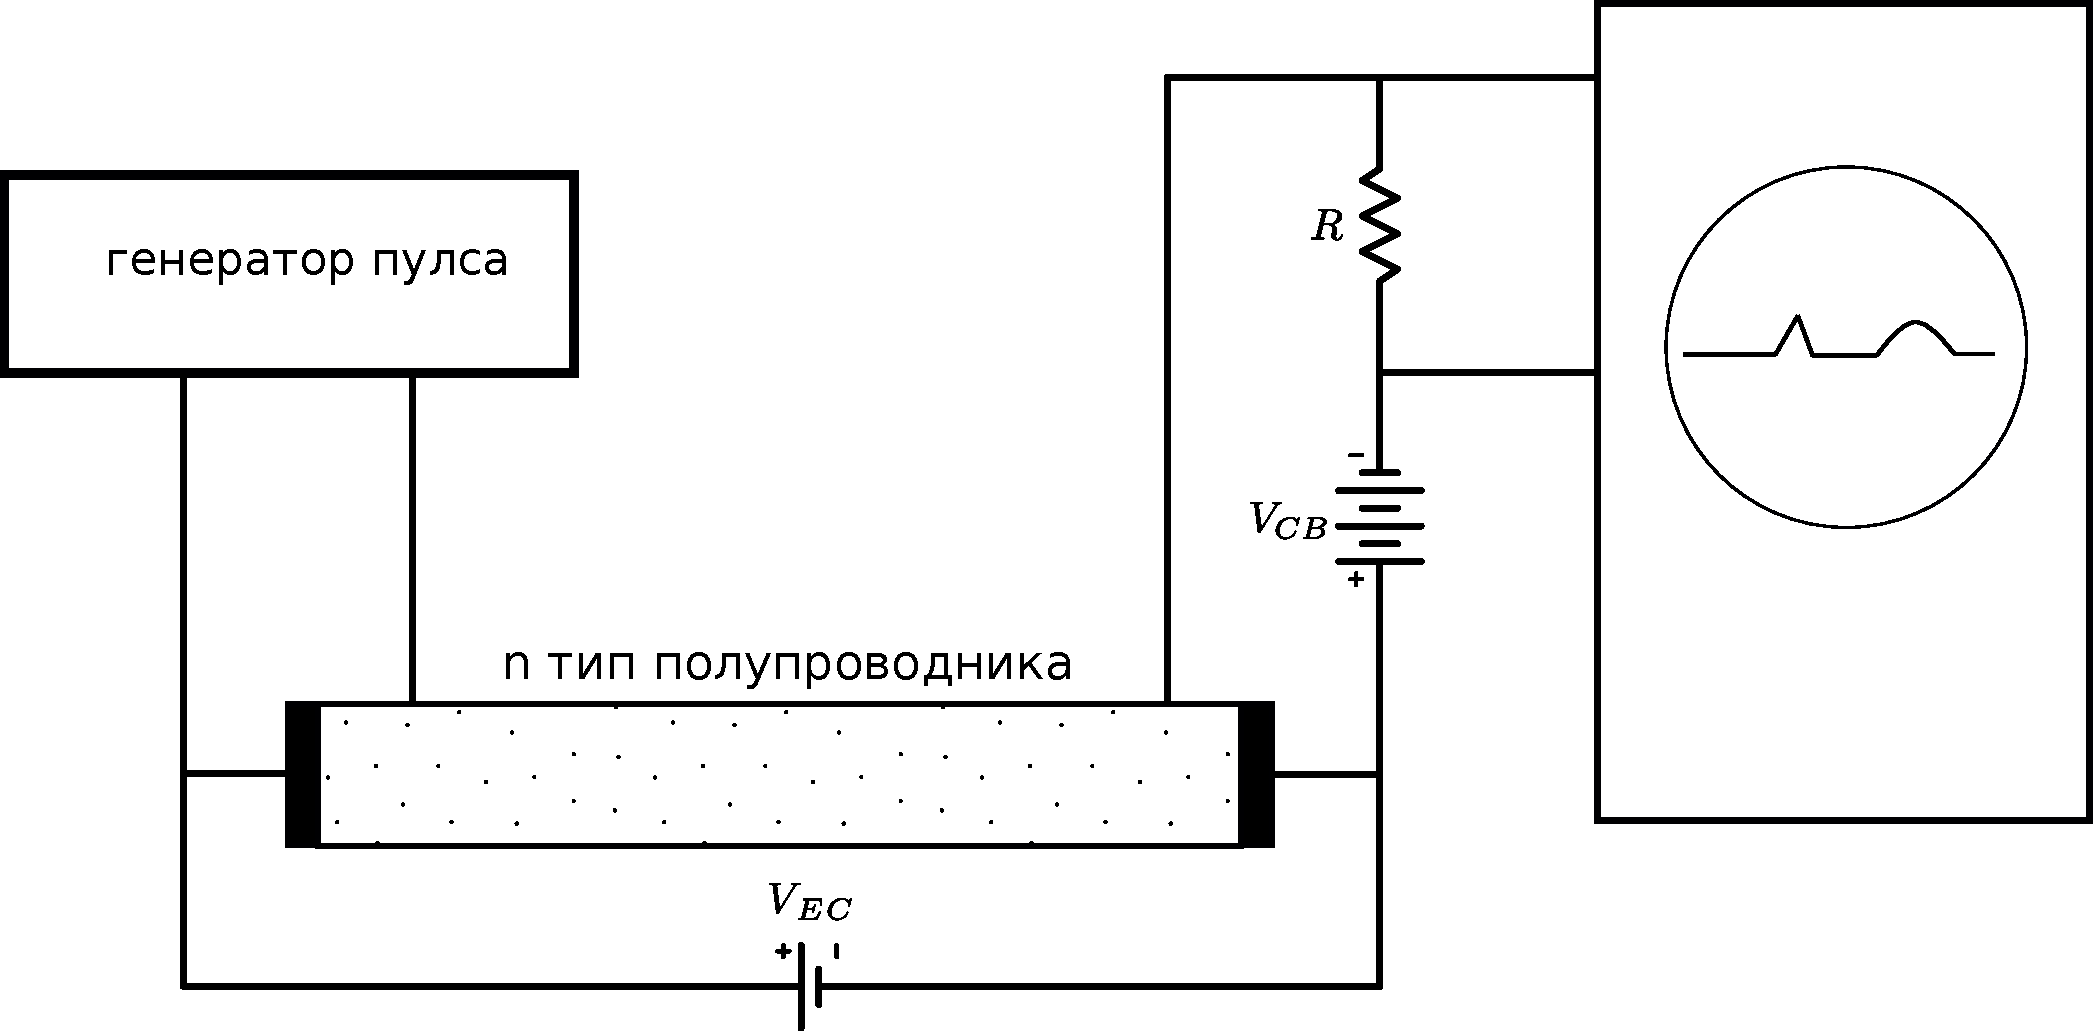
\includegraphics[width=0.8\linewidth]{Figures/experiment-sch.svg.pdf}
	\caption{Схема експеримента за посматрање дрифта и дифузије инјектованих шупљина у n - типу германијума}
	\label{fig:experiment-sch}
\end{figure}
% Овде иде слика

Експериментални аранжман, који је први пут извршен у овој форми од стране Џ. Р. Хејнс, илустрован је на сл. \ref{fig:experiment-sch} . Примерак германијума је у облику продуженог \textit{point-contact} транзистора. Ипак постоји додатни прикључак на бази. Германијум је присутан као шипка ширине у пресеку око 32 део инча, а дужине око 1 инч (\SI{1}{inch} = \SI{2.54}{cm} ).  \textit{Sweeping} поље је примењено од краја до краја шипке користећи батерију. Ово поље делује у смеру да привуче електроне са десна на лево кроз шипку. Ако се било какве шупљине појаве у шипци ићи ће са лева на десно.

Када је генератор поворке са леве стране прикључка или емитерске тачке приступа активан, емитер је поларисан позитивно, дакле у смеру у напред. Према идејама приказаним на слици \ref{fig:electron-hole-motion}, овакви услови узрокују шупљине да буду инјектоване у шипку. Потом шупљине преко шипке привлачи \textit{sweeping} поље. После неког времена доспевају у околину колектора, које како слика показује је поларисана негативно. Колектор привлачи шупљине, и неке од ових шупљина се претварају у струју која тече у колекторском делу кола. Ова струје пролази кроз отпорник и напон преко отпорника је примењен на вертикалним плочама \textit{cathode-ray} осцилоскопа. 

У радним условима, генератор пулса је остварен електронски и синхронизован са радом осцилоскопа, тако пре него што се прекидач затвори, сноп електрона у осцилоскопу крене да се помера преко цеви с лева на десно. У тренутку $t_1$ прекидач на емитеру је затворен за тренутак; време затварања је индиковано \textit{pick up} сигналом на екрану осцилоскопа. После тога ништа се не дешава до времена $t_2$ када се неке шупљине појаве на колектору; концентрација шупљина расте за тренутак и онда одумире како се група шупљина инјектује у тренутку $t_2$ прође кроз колектор. Долазак пулса на колектору није толико оштар као \textit{pick up} сигнал, зато што шупљине инјектоване у једном тренутку и на једном месту, се распрше услед дифузије тако да док група шупљина стигне на колекторски прикључак се рашири по шипци.

Овај експеримент дозвољава посматрање и мерење и дифузије и дрифта. Могуће је измерити удаљеност између две тачке и електричног поља између тих тачака; калибрисањем осцилоскопа, могуће је измерити и време пута. Тако дрифт брзина се може измерити директно, проверавајући чињеницу да поремећај који се деси на емитерској тачки. понаша онако како је за очекивати када инјектујемо мали број позитивних носилаца у шипку. Нпр. ако се удаљеност између тачака дуплира, временско кашњење између стимуланса и доласка импулса је такође дуплирано. Ово показује да носиоци имају константу дрифт брзину кроз цев. Али ако се јачина \textit{sweeping} поља дуплира, временско кашњење се двоструко скраћује. Ово показује да је брзина носилаца сразмерна електричном пољу. Ако се поларитет поља окрене, инјектовани носиоци су привучени на лево тако да ниједан не дође до колектора.

Као што је већ назначено, временски оквир доласка шупљина је мера дифузионе константе. Истраживањем зависности овог оквира времена преноса између емитера и колектора, могуће је проверавати да се шупљине распореде у складу са законима очекиваним од дифузионих феномена. Вредност ових дифузионих константи $D$ се може измерити. Ј. Р. Хејнс и његове колеге су урадили различите експерименте овакве врсте. Експериментисали су са случајем инјекције електрона у $p$ тип германијума и два одговарајућа теста за силицијум. Вредности покретности и дифузионих константи измерених овако су приказани у табели \ref{table:permeability-diffusion-constant}


\begin{table}[ht]
	\centering
	\begin{tabular}{c|cc|cc}
		\hline
		 & електрони & & шупљине &  \\
		\hline
		 & $\mu$ & $D$ & $\mu$ & $D$ \\
		\hline
		Силицијум & 1.200 & 30 & 250 & 6.5\\ 
		\hline
        Германијум & 3.600 & 93 & 1700 & 43\\ 
		\hline
        
	\end{tabular}
	\caption{Покретљивост изражена у \SI{}{\square\cm\per\volt\sec} и Дифузиона константа изражена у \SI{}{\square\cm\per\sec} } 
    \label{table:permeability-diffusion-constant}

\end{table}

Требало би напоменути да из табеле \ref{table:permeability-diffusion-constant} однос између дифузионе константе и пермеабилности је отприлике 1/40. а димензије ових квантитета је у волтима. Другим речима, однос $D$ и $\mu$ je \SI{25}{\milli\volt}. Ова вредност има фундаментални значај, јер веза између $D$ и $\mu$ се обично назива Ајнштајнов однос. Ова веза је скоро била детаљно истражена, на начин описан пре за германијум. Значај вредности је да електрон који се креће са неком \textit{random} термалном енергијом ће, у просеку моћи да преброди потенцијалну препреку од \SI{25}{\milli\volt}. Другим речима \SI{25}{\milli\volt} је електростатички потенцијал који одговара термалној енергији једног електрона. Може се рећи да ако је електрон у покрету са термалном енергијом у супротном смеру од електричног поља, када се помери за \SI{25}{\milli\volt} његова брзина ће постати 0 и почеће да се креће у супротном смеру. Чињеница је да је вредност од \SI{25}{\milli\volt} добијена показује ад носиоци који се крећу дрифтом и дифузијом у Хејнсовом експерименту електрони. Када би била половина или двострука вредност, нпр, однос $D$ и $\mu$ би био \SI{12.5}{\milli\volt} или \SI{50}{\milli\volt}.

Када се Хејнсов експеримент први пут изводио, процедура се разликовала постављањем прикључака на супротне стране филамента и коришћењем филамента далеко веће ширине него дебљине. Ови експерименти указују да је интеракција између ових прикључака се одвијала кроз \textit{bulk}, а не преко површине.


\subsection{Врући електрони и Омов закон}

Још један фундаментални експеримент о понашању електрона и шупљина полупроводника има извор из практичног истраживања. Негде током 1948. постојао је покушај да се полупроводници користе као појачавачи на високим учестаностима, наишао сам на идеју коју је независно открио и објавио као \textit{Staueffekt}, Х. А. Кромер. Кромер није узео у обзир појачавање и његова употреба је први пут објављена 1954. године.

\begin{info}
    \textit{Staueffekt} преведено са немачког значи ефекат загушења. 
\end{info}


Основни принцип \textit{Staueffekt} се може разумети овако: шупљина у валентном \textit{band}-у ће изгубити енергију фононима максималном брзином $P(max)$ када је његова енергија негде близу средине овог \textit{band}-а. Ако се примени електрично поље, његова дрифт брзина $v_d$ мора бити ограничена:

\begin{equation}
    q E v_d < P(max)
\end{equation}

пошто не може да добија енергију бесконачно. Пта се дешава са више детаља: Ако шупљина добије превише енергије, креће се нижа стања у валентном \textit{band}-у тако да његова ефективна маса промени знак тако да се успорава уместо да се убрзава од стране електричног поља.

\begin{info}
    Извор википедија - Фонон у физици је назив за вибрације између атома или молекула кристалне решетке. На основу честичне слике, фонон се може посматрати као квазичестица у кристалу као последица вибрационог кретања. Пошто не може постојати самостално, независно од кристалне решетке у којој постоје вибрације између атома, фонон није честица, већ спада у квазичестице. 
\end{info}

Негативне отпорности нису пронађене. Ипак експерименталне околности које су створили Е. Ј. Рајдер и В. Шокли у којима су \textit{random} енергије шупљина и електрона су повећане на ниво еквивалентне температуре од неколико хиљада степени. Ови ефекти представљају фундаменталну девијацију од Омовог закона у смислу да они настају само од јачине електричног поља, а не од споредних ефеката као промена броја шупљина и електрона услед промене температуре.

Зависност дрифт брзине шупљина и електрона зависи од електричног поља. Иако генералне особине ових карактеристика су познате, нису квантитативно објашњене. Разлика између једноставне теорије и експеримента долазе од комплексе структуре површинских енергија за шупљине и електроне, односно од одступања од модела једне ефективне масе полупроводника.

Из практичног погледа, нелинеарности у дрифт брзинама су битне у рачунању карактеристика полупроводничких уређаја.

\subsection{\textit{pn} - спој и појединачни кристали}

Исправљање контаката од главног значаја у раном проучавању транзисторске физике, су прављени притискањем шиљатих жица на полупроводник и потом форматирањем их пуштајући високу струју. Било је тешко тада разумети ове процесе са становишта атома, а тако је и данас.

Битна одлука у години након открића транзистора је била да ли треба се  концентрисати на \textit{p-n} спојеве унутар полупроводника, а не на тачкасте контакте. Из ранијих радова познато је да су такви спојеви исправљачки или осетљиви на светлост. Ипак, њихове карактеристике нису потпуно јасне на нивоу атомских модела. Пошто \textit{p-n} спој  може да се направи у једном кристалу мењањем састава примеса од донора за \textit{n}-тип полупроводника до акцептора у \textit{p} типу, много је једноставнија структура од метал-полупроводник контакт и њено понашање је предвидиво из теоретског гледишта. Чинило се логично, дакле, покушати разумети \textit{p-n} спој и тачкасте контакте касније.

Још један разлог одабира \textit{p-n} спојева као централне теме је могућност производње транзистора заснованог на \textit{p-n} спојевима, објављено је 1949. године.

\textit{p-n} спој је најједноставнија такозвана композициона структура полупроводничке електронике. Под композициона структура подразумева се један кристал полупроводника где композиција донорских и акцепторских примеса се мења на системски и контролисан начин. Пре него што објасни теорију понашања \textit{p-n} споја, хтео бих да кажем нешто о начину на који је понашање \textit{p-n} спој било задовољавајуће са теоретског гледишта оствареног у Бел Телефон Лабораторијама. Историја овог примера је интеракција практичних потреба и истраживачког програма.

На почетку, билу су покушаји, посебно од М. Спаркса, да се произведе \textit{p-n} спој на друге начине, али особине тих спојева нису успеле да испуне теоретска очекивања. (Проблеми су скоро увек били због чистоће - значај бакра није био знан у то време.)


\begin{figure}[ht!]
    \centering
	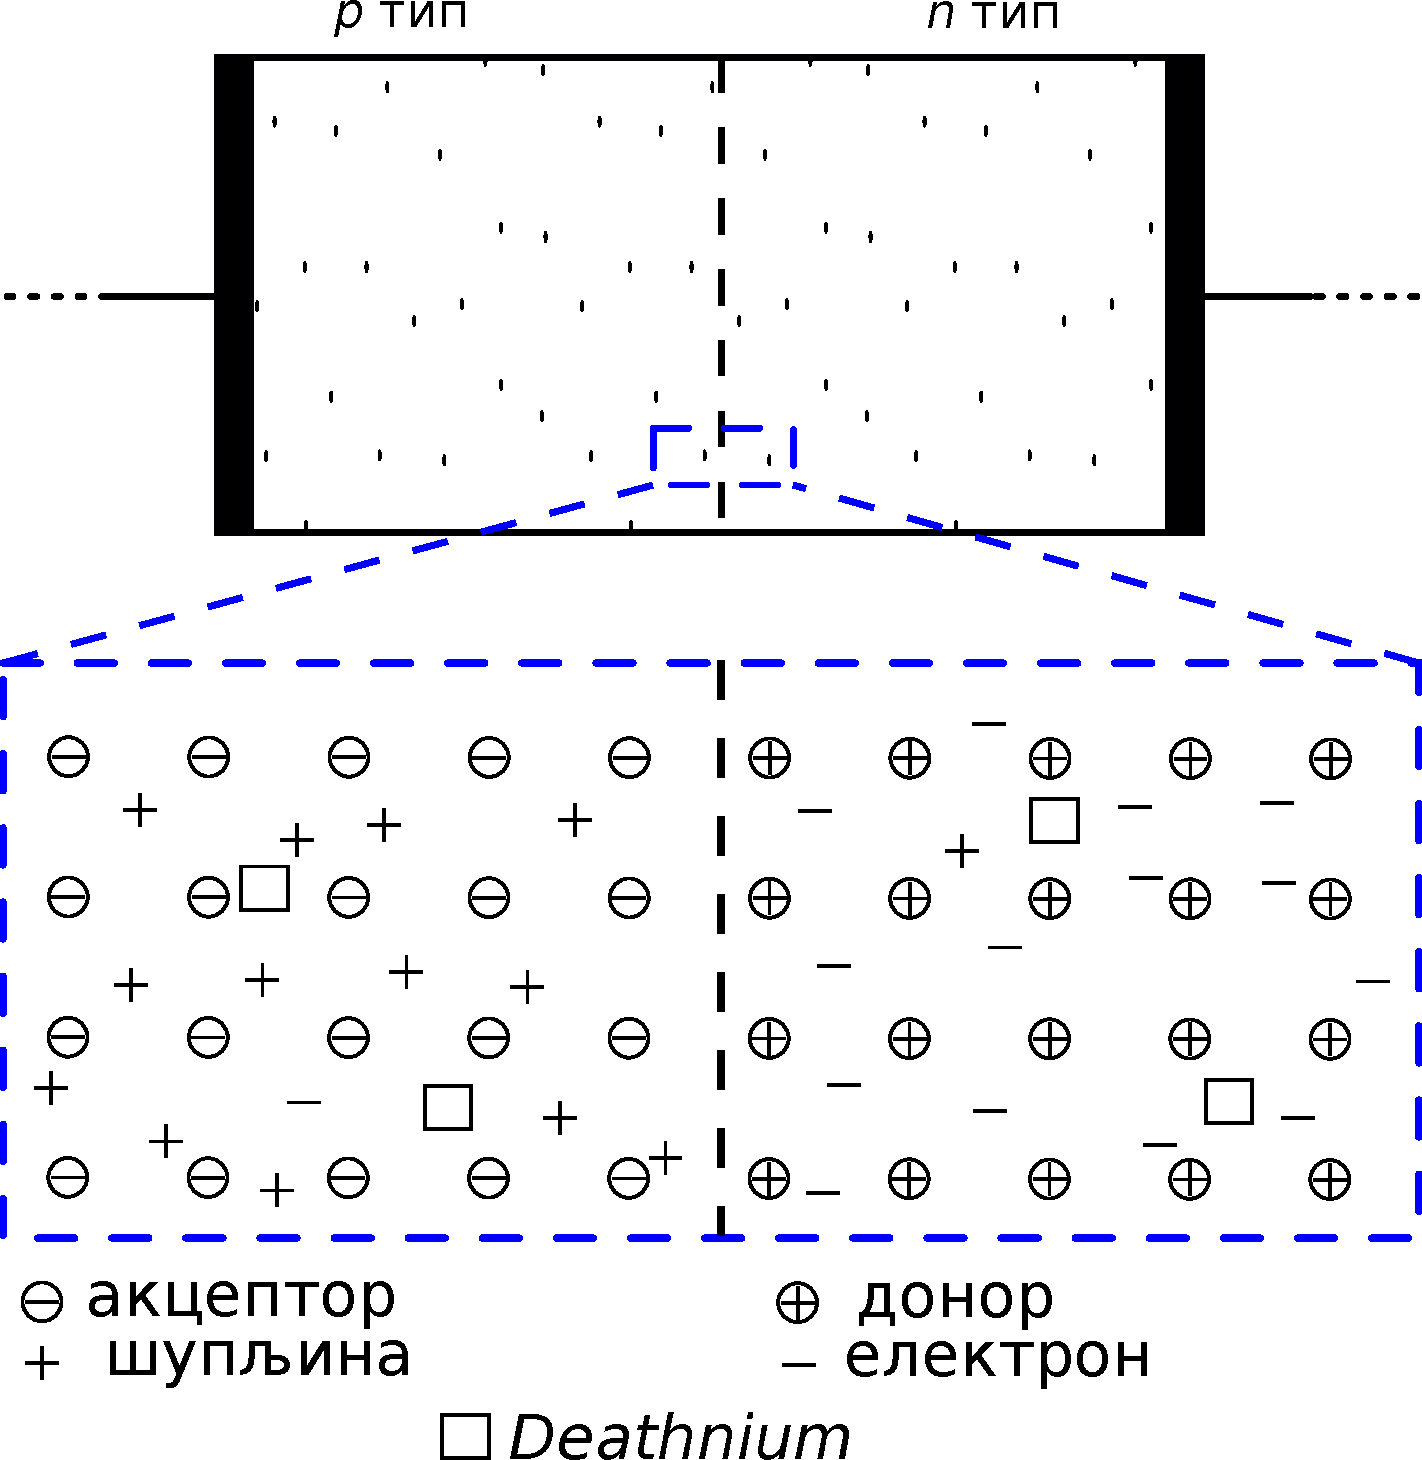
\includegraphics[width=0.7\linewidth]{Figures/pn-junction.pdf}
	\caption{\textit{p-n} спој и расподела несавршенства у њему. (Зарад једноставности, компензовани парови донора и акцептора нису приказани.)}
	\label{fig:pn-junction}
\end{figure}
% Овде иде слика



Као резултат потреба истраживачког одељења за униформним материјалом за потребе прављења експерименталних транзистора, програм је направљен за развој великих кристала германијума. Интересантно је напоменути да стварна одлука и фокус овог програма је био услед принципијелност Ј. А. Мортона, који је водио групу за развој транзистора, а не од стране моје групе или других истраживачких група. Осећао сам у то време да научне студије би могле адекватно да се изведу скраћивањем малих примерака из поликристалних монолита материјала. Као резултат Мортоновог притиска, Г. К. Тил, сарађујући са Ј. Б. Литлом, је направио експериментални апарат за чупање појединачних кристала германијума из комада германијума грејаног у графитном лонцу у који се потопи мало кристално "семе". Скорији напредак у транзисторској науци и технологији је заснован на овим кристалима. Додавање акцептора у комад \textit{n}-типа током извлачења како би га претворили у \textit{p}-типа је дало прве добре \textit{p-n} спојеве.

Још један веома значајан напредак у припреми материјала би требало да се помене. Ово је метод делимичног пречишћавања је открио В. Г. Пфан, такође из Бел Телефон Лабораторија. Напомена да  нечистоће често могу бити склоније растварању у растопљеном германијуму него кад је у чврстом стању. Пфан је осмислио систем понављања прочишћавања кристализацијом. Прављењем продуженог графитног лонца и омогућавањем да се загреје само одређена дужина или део, он је успео да растопи делове сукцесивно са једног краја на други и померити нечистоће из великог дела кристала тако што се концентришу само на једном крају. На овај начин германијум кристала има атом нечистоће за сваких $10^{10}$ атома германијума који се произведу. Густина нечистоћа у овим кристалима је поредива са густином молекула у гасу под притиском од $10^5$ \SI{}{\milli\meter} живе. Прикладно је назвати парцијално пречишћавање - вакуумском пумпом за транзисторску електронику. 

Слика \ref{fig:pn-junction} представља \textit{p-n} спој. У расправи о његовим електричним особинама, бавићемо се са 5 врста несавршенства који су приказани на доњем делу слике. Из механичког гледишта кристал је хомоген и савршен. Типична концентрација нечистоћа у кристалу може бити $10^{15}$ \SI{}{\per\centi\meter\cubed}. Ова густина нечистоћа је тако мала да би један мога да прође кроз цео ред атома са једног краја кристала на други и да прође кроз у просеку 10 несавршености. Дакле кристална структура је само мало промењена  што се тиче несавршености. Са електричног гледишта несавршенства имају велики ефекат.

Као што је приказано на слици \ref{fig:pn-junction} електрони се могу наћи у \textit{n}-типу где неутралишу хемијски простор наелектрисања, а шупљине су присутне на сличан начин у полупроводнику \textit{p}-типа. Како би се ситуација одржала, под условима термалног еквилибријума, мора постојати електрично поље присутно у кристалу. Идеја поља присутног у полупроводника под условима термалног еквилибријума је на први поглед изненађујућа. Ипак неопходност за овакво електрично поље. се може видети из услова са слике \ref{fig:pn-junction}. Претпоставимо да не постоји електрично поље преко споја, онда због дифузије шупљине ће прећи преко споја са лева на десно и слободни електрони ће слично дифузијом прећи преко споја с десна на лево. Као резултат, постојаће пренос позитивних наелектрисања  на десно преко споја. Настаће електрично поље таман толико да спречи даљи ток струје.

\begin{figure}[ht!]
    \centering
	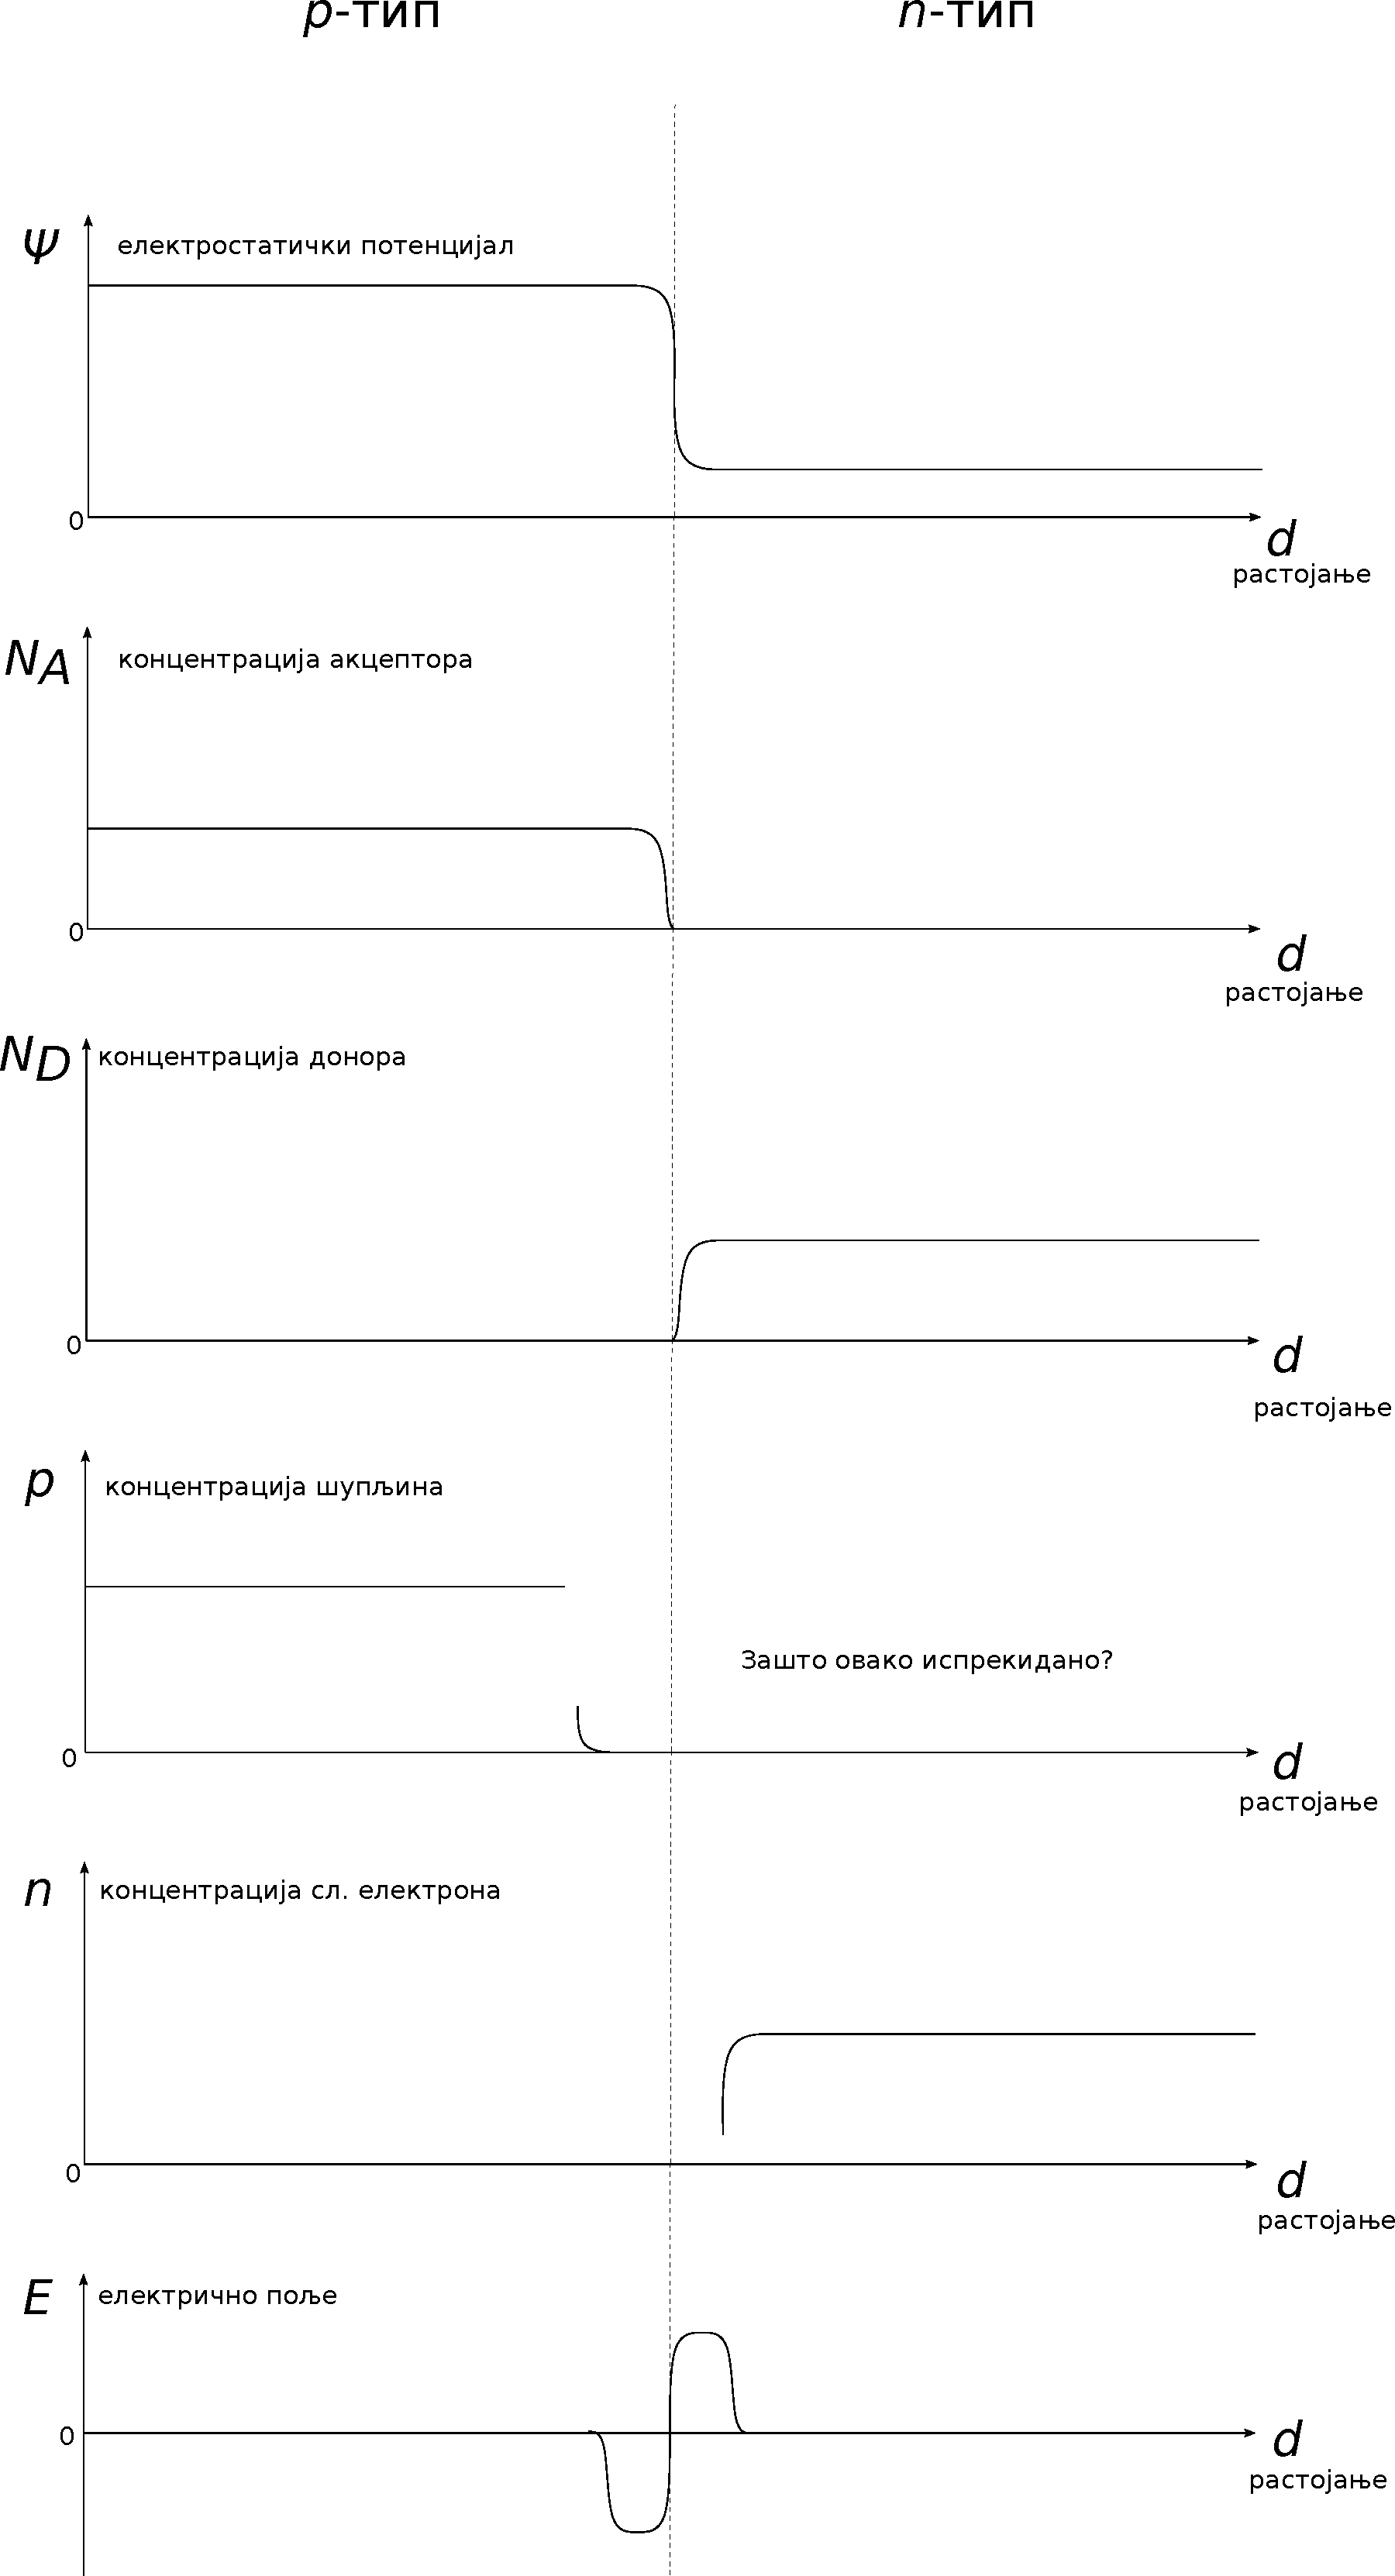
\includegraphics[width=0.5\linewidth]{Figures/potential-charge-dist.pdf}
	\caption{Потенцијал и расподела наелектрисања у \textit{p-n} споју}
	\label{fig:potential-charge-dist}
\end{figure}
% Овде иде слика


Електрично поље \textit{p-n} споја се појављује на слици \ref{fig:potential-charge-dist} (а) у виду електростатичког потенцијала $\psi$. Остали делови слике показују како електрично поље и електростатички потенцијал долазе од концентрација наелектрисања који су присутни. Хемијско наелектрисање је приказано делом у (б) и (в) ове слике . На овом примеру приказано је $N_d$ и $N_a$ карактеристика, тако да се пренос из \textit{n}-типа у \textit{p}-тип дешава нагло на месту споја и таква компензација једне примесе другом није укључена. У присуству електростатичког потенцијала приказаног у делу (а) слике \ref{fig:potential-charge-dist} шупљине су обично одгурнуте у лево. Као резултат, концентрација шупљина опадне до неке мале вредности пре него што се дође до споја. Електрони имајући негативно наелектрисање се обично крећу у тачке високог електростатичког потенцијала, тако да се не могу наћи у близини споја. Као последица, хемијско наелектрисање концентрација се не компензује шупљинама или електронима у близини споја. Тако електростатички диполни део се ствара на споју, концентрација наелектрисања као што се види у делу (е) слике \ref{fig:potential-charge-dist}. Диполни слој је неопходан како би се створи електростатички потенцијал приказан у делу (а).

Математички оно што је урађено како би се одредио облик електростатичког потенцијала на слици \ref{fig:potential-charge-dist} (а) је решавање диференцијалне једначине. Ако се зависност од електростатичког потенцијала према растојању као непозната, одатле и одређених принципа статистичке механике могуће је написати израз за концентрацију наелектрисања услед шупљина и електрона. Ове концентрације наелектрисања се могу повезати са хемијским несавршеностима како би се добила диференцијална једначина за електростатички потенцијал. Диференцијална једначина је Поисонова једначина, која се односи на изводе електростатичког потенцијала у концентрацију наелектрисања. Решавањем једначине добија се да \textit{p-n} спој у термалном еквилибријуму је представљен као на слици \ref{fig:potential-charge-dist}.

Под условима термалног еквилибријума никаква струја нити шупљина нити електрона неће тећи кроз спој. Ово је предност, али треба узети у обзир да еквилибријум долази од струја које се поништавају. Илустроваћемо ово сматрајући ток шупљина напред и назад преко споја. Иако концентрација шупљина је мала у \textit{n}-типу и даље игра кључну улогу у понашању \textit{p-n} споја. Узмимо у обзир путању шупљине која доспева у полупроводник \textit{n}-типа пењући се потенцијално "брдо" илустровано на слици \ref{fig:hole-current}. Попећи се на брдо и стигавши на плато константног електростатичког потенцијала , наставиће да се креће кретње случајном дифузијом. Највероватнији исход овог кретања је да ће се спасти са брда и склизнути назад у \textit{p}-тип. Нећемо се бавити шупљинама са овим исходом. Са друге стране, могуће је да дифузијом оде дубље у \textit{n}-тип. У овом случају има ће просечно време дифузије $\tau$, и затим ће бити заробљено од стране \textit{Deathnium} центра који ће га рекомбиновати са електроном.

% Ово теорија о неопходности \textit{Deathnium} центра да се шупљина рекомбинује не делује да је заживела.

\begin{figure}[ht!]
    \centering
	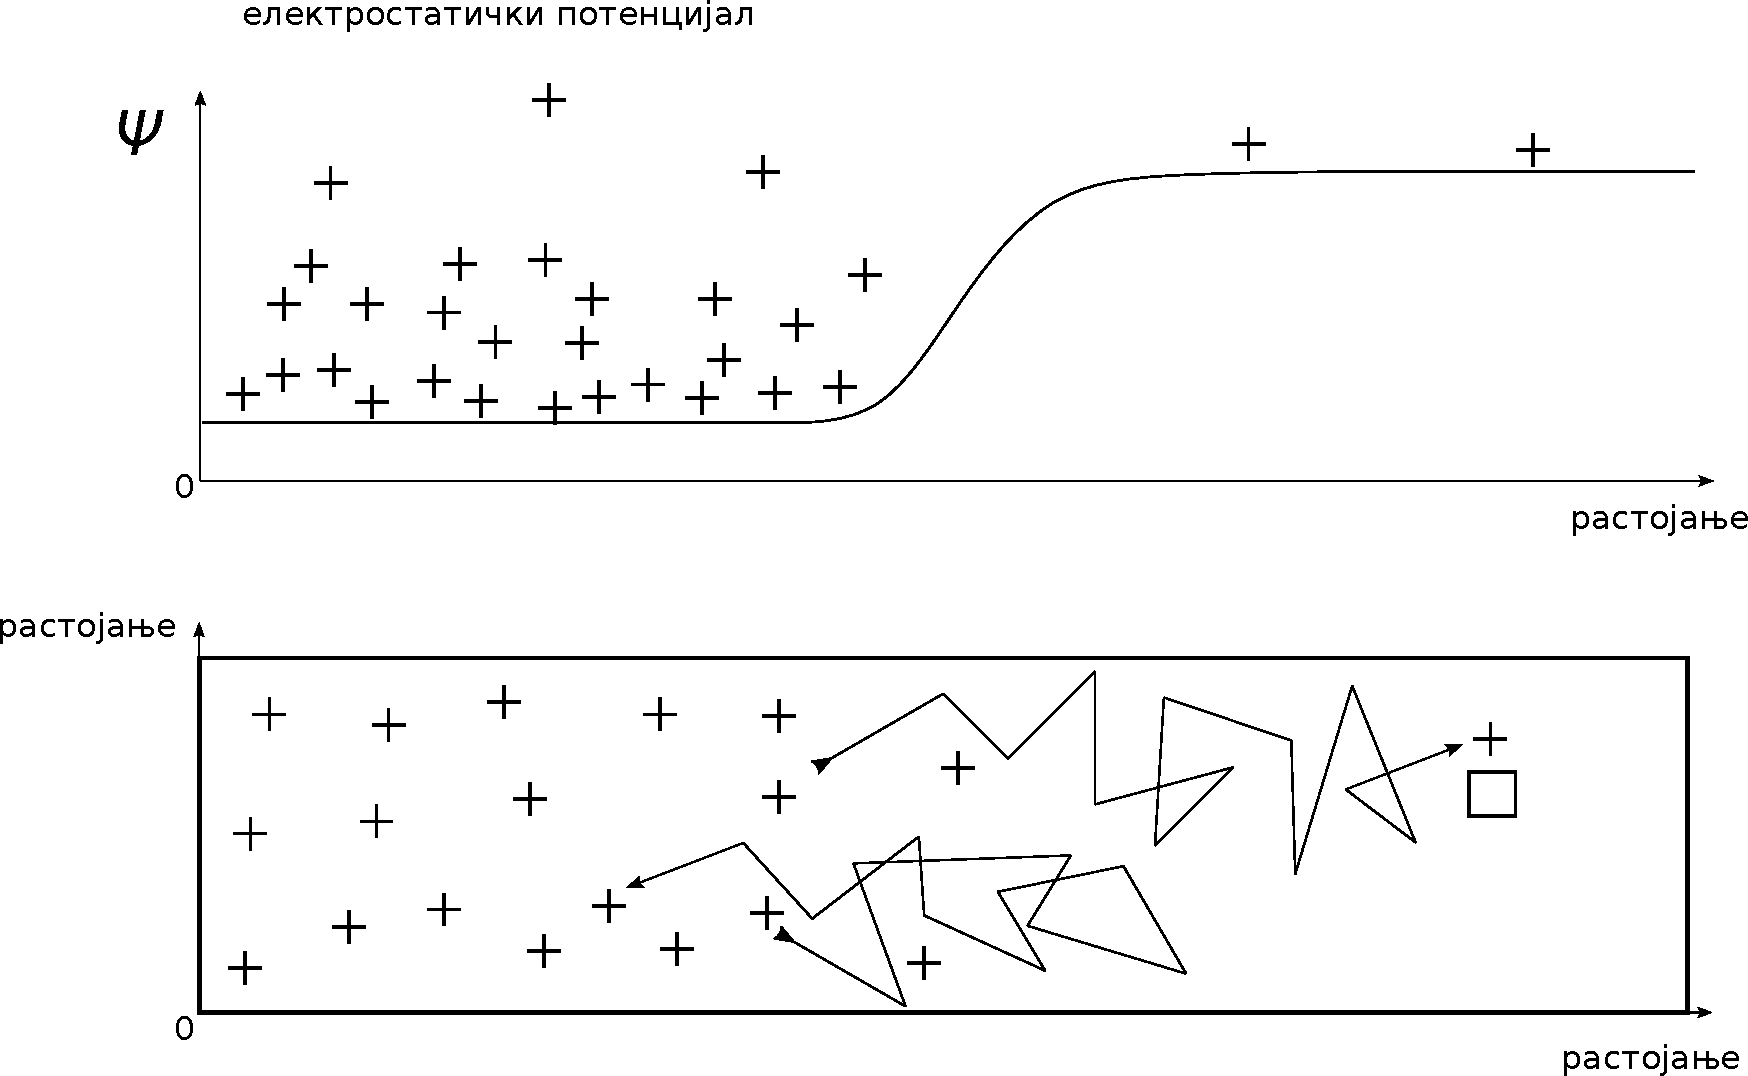
\includegraphics[width=0.8\linewidth]{Figures/hole-current.pdf}
	\caption{Струја шупљина из\textit{p} у \textit{n} део \textit{p-n} споја}
	\label{fig:hole-current}
\end{figure}

Просечна дубина до које шупљине дођу дифузионим кретањем у \textit{n}-типу зависи од њиховог животног века. Шупљине се расипају дифузијом у полупроводнику. Када се одговорајућа диференцијална једначина која описује процес реши, пронађено је просечна дубина до које се пробију је дата једначином:

\begin{equation}
	L=\sqrt{D_p\tau}
\end{equation}

где је $L$ позната као дифузиона дужина, $D_p$ дифузиона константа за шупљине, $\tau$ животни век шупљина у \textit{n}-тип региону. Тако под условима еквилибријума струја шупљина тече од \textit{p} дела ка \textit{n} и пробије се у просеку за једну дифузиону дужину пре него што се рекомбинује са електронима.

Под условима еквилибријума \textbf{принцип детаљног баланса} је одржан. Овај принцип статистичке механике каже да сваки процес и њему супротан се дешавају једнако често. Зато морамо закључити да ток шупљина из \textit{p} дела ка \textit{n}, где се рекомбинују, је праћен супротним процесом. Супротни процес је термална генерација шупљина кроз \textit{Deathnium} центре, праћена дифузијом до споја где склизну у \textit{p} део.

\begin{figure}[ht!]
    \centering
	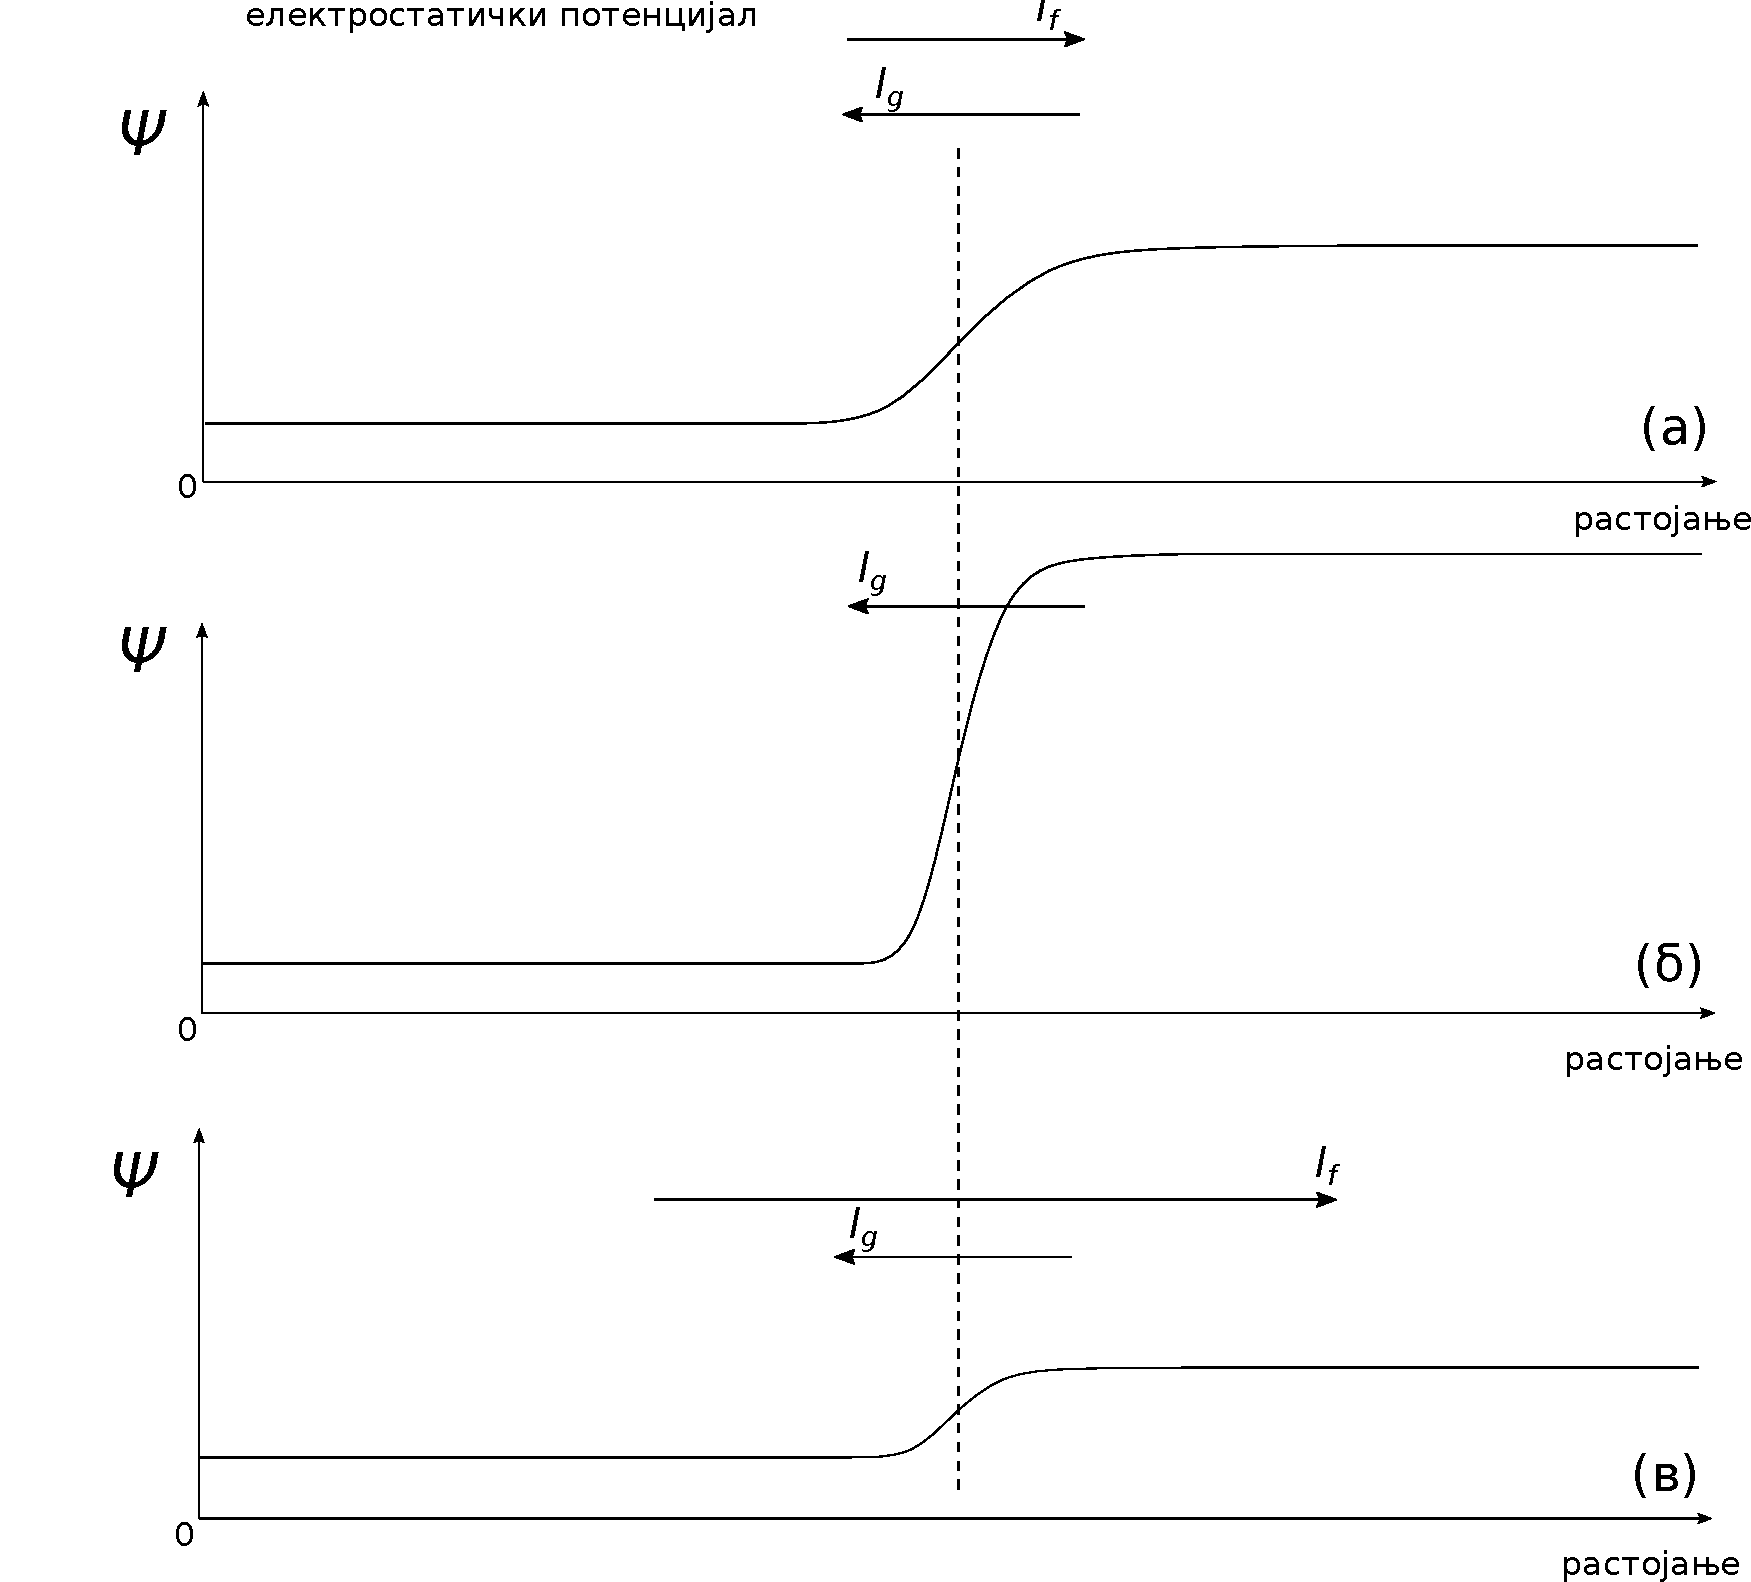
\includegraphics[width=0.8\linewidth]{Figures/dependence-recomb-gen.pdf}
	\caption{Зависност струја рекомбинације и генерације од поларизације (а) термални еквилибријум (б) \textit{reverse} (в) у напред}
	\label{fig:dependence-recomb-gen}
\end{figure}

Примена напона на прикључке направе приказане на слици \ref{fig:pn-junction} уништава тачни баланс две струје о којима смо расправљали. У разматрању примене напона занемарићемо падове напона на контактима између металних електрода да слици \ref{fig:pn-junction} и полупроводника. На крају овог дела текста вратићемо се на кратко разлозима зашто је могуће занемарити ове  падове напона. Утицај примене напона је приказан на слици \ref{fig:dependence-recomb-gen}. У делу (а) ове слике показан је у условима термалног еквилибријума. Де струје које смо претходно поменули су представљене као $I_f$ и $I_g$, где представљају, респективно, струје шупљина које улазе у \textit{n} део и рекомбинују се и струје генерисане у \textit{n} делу тако да дифузијом крећу према споју. Ознаке \textit{f} и \textit{g} могу да се односе на називе \textit{forward} и генерацију. Ово комбиновани избор избегава ознаку \textit{r}, кој се може односити и на \textit{g} и на рекомбинацију. У овој одлуци \textit{forward} је еквивалентан рекомбинацији, а генерација је једнака \textit{reverse}. У делу (б) слике ситуација за јаку \textit{reverse} поларизацију , негативни напон је примењен на \textit{p} и позитивни напон на \textit{n} део споја, тако да разлика електростатичког потенцијала између \textit{p} и \textit{n} се повећа. Ако је електростатички потенцијал довољно висок, одговарајућа ситуација је приказана у делу (б), где практично ниједна шупљина не може да се попне уз брдо потенцијала и струја $I_f$ скоро падне на 0. Ово је приказано тако што је $I_f$ приказана као да је занемарљиве дужине, док је $I_g$ практично исте дужине као у еквилибријуму. Уопштено, дифузиона дужина $L$ је много дужа од дужине дипола или наелектрисаног простора (?). Отуда простор одакле $I_g$ потиче је практично непоремећен супротном поларизацијом и $I_g$ је имуно на \textit{reverse}  поларизацију. Ова независност струје од поларизације се назива \textbf{сатурација}.

% space-charge region је вероватно област просторног товара.

% Струја генерација се обележава са I_s као струја сатурације.

Када је поларизовано унапред, илустровано на слици \ref{fig:dependence-recomb-gen} (в) $I_f$ се повећава. Ово повећање је описано у виду енергетске разлике за шупљину у \textit{n} у \textit{p} део. Ова енергетска разлика је једнака наелектрисању електрона помножено са разликом електростатичких потенцијала између две стране. Можемо применити генералну теорему статистичке механике у разматрање броја шупљина које ће имати довољно енергије да се попну уз брдо потенцијала. Ова теорема тврди да сваки пут када се брдо повећа за једну термалну јединицу енергије, $kT$ број шупљина које се могу попети уз то више потенцијално брдо је смањено за фактор од $I/e$. Пошто потенцијална баријера је већ присутна у условима термалног еквилибријума, исто важи и за спуштање баријере за вредност од $kT$ ће повећати струју за фактор од $I/e$. Промена висине баријере узрокован од стране примењеног напона $V$ је $-qV$, где је поларност изабрана тако да позитивне нивои се односе на позитивне потенцијале примењене на \textit{p} део и $q$ је апсолутна вредност наелектрисања једног електрона. Еквилибријум је за $V=0$, и ово је случај када је $I_f = I_g$. Уопштено струја рекомбинације:

\begin{equation}
	I_f = I_g e^{\dfrac{qV}{kT}}
\end{equation}

ово даје пораст тоталне струји шупљина из \textit{p} и \textit{n}, тако да је разлика:

\begin{equation}
	I_f - I_g = I_g (e^{\dfrac{qV}{kT}} - 1)
\end{equation}

Струја је једнака 0 за $V=0$, повећава се експоненцијално за велике вредности позитивног напона $V$, а смањује се у негативну сатурацију за $I_g$ $V$ је негативно и много веће него $kT/q$.

Слично резоновање се може применити на струју електрона која тече кроз спој. Примењен потенцијал смањује потенцијалну баријеру за шупљине, очигледно је смањује за електроне, као последица, велике струје електрона теку под истим условима који производе велике струје шупљина. У оба случаја велике струје одговарају току мањинских носиоца у оба дела\textit{p-n} споја. И у оба случаја преноси се позитивно наелектрисање из \textit{p} дела у \textit{n} део. У једном случају пренос је позитивних несавршености, под именом шупљине \textit{p} у \textit{n}, а у другом пренос негативних несавршености, електрона из \textit{n} у \textit{p}. За случај обрнуте поларизација и потенцијала који рате, шупљине остају у \textit{p} делу, а електрони остају у \textit{n} делу. Сатурациона струја услед генерације у оба региона тече. Ако се тотална струја сатурације назива $I_s$, онда ће тотална струја за било коју примењени напон $V$ дата једначином:

\begin{equation}
	I = I_s(e^{qV/kT}-1)
\end{equation}

% Карактеристика исправљања \textit{p-n} споја постоји као слика у оригиналном раду.

Очигледно $I_s$ је једнака суми две струје генерације. Једначина задовољава \textit{p-n} спој у германијуму, и доказана је мерењима. Треба напоменути да раздвајањем \textit{forward} и \textit{reverse} струја се добија се фактор $e$ када је напон $kT/q=$ \SI{25}{\milli\volt}. Представља тачно фактор који је предвиђен претходном једначином. Ово слагање теорије и експеримента је доказ да се несавршености које чине струју \textit{p-n} споја имају наелектрисање електрона. Када би имали двоструко наелектрисање, вредност би била \SI{12.5}{\milli\volt}; да је пола наелектрисања било би \SI{50}{\milli\volt}. За веома \textit{forward} поларизоване спојеве, потенцијална баријера између \textit{n}-типа и \textit{п}-типа је елиминисана. Под овим условима висока концентрација мањинских носилаца прелази преко баријере и концентрација већинских носилаца може бити значајно поремећена. Под овим условима није више тачно да се мањински носиоци дифузионо крећу у делу без поља, као што је случај када  концентрације носилаца сличне еквилибријуму постоје. Иако ови услови великих снага су од општег интереса, нећемо их даље разматрати овде.

Постоји велики број начина на који се теорија дифузије за исправљање код \textit{p-n} спојева може експериментално тестирати. Узећемо у обзир тест заснован на фотолектричном ефекту. Фотони довољне енергије могу да створе шупљина-електрон парове када се апсорбују у германијуму. Ова генерација се додаје на термалну генерацију унутар \textit{deathnium} центара. Ако се светлост усмери на примерак у облику мале тачке, онда је могуће генерисати мањинске носиоце у том малом делу на прецизној удаљености од споја. Струја која тече кроз спој је резултат генерације услед светлости би се смањила ако повећамо удаљеност светлосног извора од споја. Може се показати да вероватноћа да се мањински носилац генерише на удаљености $x$ од споја дифузионо креће ка споју пре него што се рекомбинује је једноставно:

\begin{equation}
	e^{-\dfrac{x}{L}}
\end{equation}

где је $L$ дифузиона дужина мањинског носиоца у делу у коме је генерисан. Ова експоненцијална зависност побуде на удаљеност од споја је директно проверен од стране Гаушера и његових колега. Пронашли су вредност $L$ одређену истраживањима се слаже са потребом за објашњењем вредности $I_s$ у формули исправљања.

Уа потребе илустрације можемо узети у обзир вредност дифузионе дужине. Типичан животни век мањинског носиоца је $10^{-4}$\SI{}{\sec} и дифузиона константа за електроне у германијуму је \SI{93}{\centi\meter\squared\per\sec}. Од ових вредности се добија дифузиона дужина од око \SI{0.1}{\centi\meter} или \SI{1}{\milli\meter}.

Пошто се светлост понаша као струјни генератор, његови ефекат може бити укључен у еквивалентно коло за  \textit{p-n} спој. Ово је илустровано на слици \ref{fig:equi-photocell}. Овде $I_l$ је струја мањинских носиоца генерисани светлошћу. Еквивалентно коло одговара случају у коме је светлост усмерена на удаљеност $x$ од споја. Ако се светлост поремети, одговарајућа просечна вредност фактора експоненцијалне зависности би требало да се користи. Ако светлост пада и на \textit{p} и на \textit{n}, ова просечна вредност би требало да узима у обзир да дифузиона дужина за шупљине у \textit{n} региону је вероватно различита од електрона у \textit{p} региону. Слика \ref{fig:equi-photocell} наглашава значај разматрања светлости које делује као струјни генератор. Ако се еквивалентно коло са слике \ref{fig:equi-photocell} стави у отворену везу, онда ће настати фотонапон. Овај фотонапон који је генералном случају  је нелинеарна у зависности према јачини светлости због исправљајући карактеристика исправљача. У еквивалентном колу са слике \ref{fig:equi-photocell}, ипак струјни извор је линеаран према јачини светлости. Ова независност струјног извора од напона примењеног на \textit{p-n} споју је верификована за велики број експерименталних услова од стране Гaушера, његових колега, и Питенпола.

% Превод за фотонапон да ли је добар? и повезаност са photovoltaic PV ћелијама које се користе код соларних панела.

% Шта значи исправљање у овом смислу 

\begin{figure}[ht!]
    \centering
	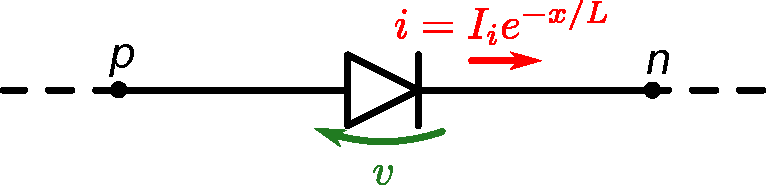
\includegraphics[width=0.8\linewidth]{Figures/equi-photocell.pdf}
	\caption{Еквивалентно коло за \textit{p-n} спој фотоћелије}
	\label{fig:equi-photocell}
\end{figure}

\subsection{Биполарни транзистор}

Биполарни транзистор је композициона структура се састоји од два \textit{p-n} споја наслоњених један на други. Генерално понашање као појачавачке направе, биполарни транзистор показује доста сличности са триодама електронских цеви (\textit{vacuum tube}, или термионски вентил. Слика \ref{fig:structure-junction-transistor} показује \textit{n-p-n} биполарног транзистора у појачавчком колу, транзистор који је облику сендвича са слојеве германијума \textit{p} типа уметнутог између два слоја германијума \textit{n}-типа. Неисправљачки електрични контакти су направљени ка сва три слоја. Под радним условима регион \textit{n}-типа са десне стране, познат као колектор, је поларисан позитивно како би привукао електроне. Као резултат, супротна поларизација се појављује између њега и уметнутог слоја, познатог као база. Струја која тече преко обрнуто поларисаног споја може бити контролисана преко сигнала између слоја базе и слоја \textit{n}-типа десно који се назива емитер. Као што ће бити после детаљно објашњено, поларизација на емитеру се понаша као регион измећу катоде и мреже (\textit{grid}) у електронској цеви. Велика вероватноћа је да електрони који уђу преко базе дифузијом дођу до контакта за колектор , и тако ток електрона од емитер до колектора се може контролисати потенцијалом преко емитер-база прикључака. Ово је веома слично контролисању катоде до аноде код термионских триода.

% термионска триода

\begin{figure}[ht!]
    \centering
	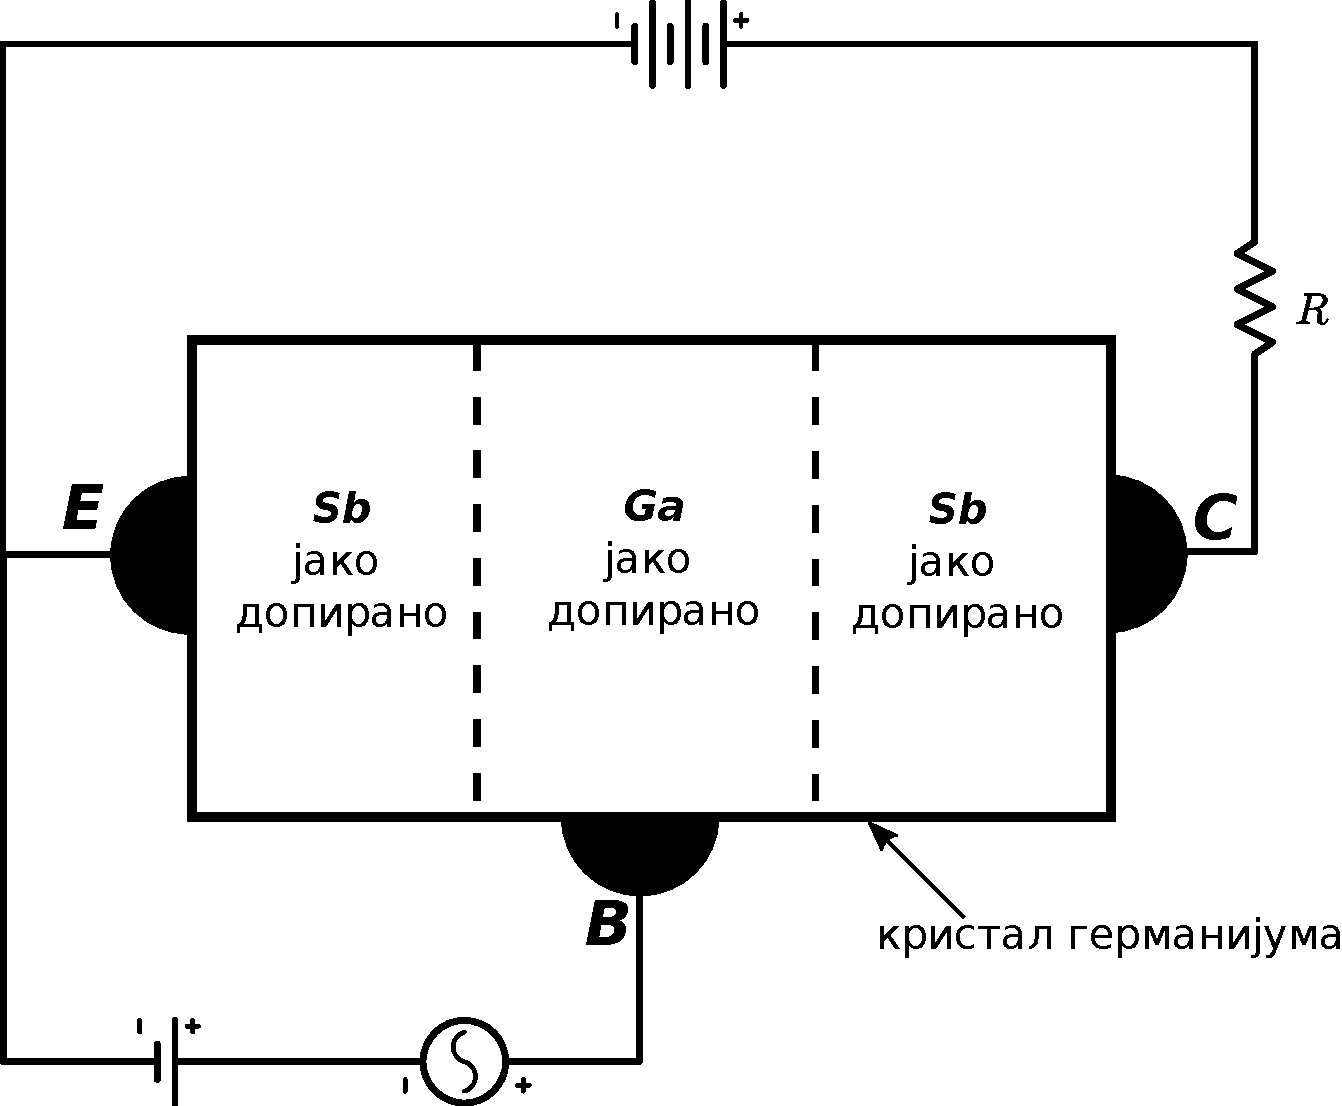
\includegraphics[width=0.6\linewidth]{Figures/structure-junction-transistor.pdf}
	\caption{Структура биполарног транзистора и поларизације-напајања за његово дејство као појачавачко коло}
	\label{fig:structure-junction-transistor}
\end{figure}

Биполарни транзистори се могу произвести на различите начине. Композициона структура се може произвести у машинама које развијају кристале техникама које су коришћене за једноставне \textit{p-n} спојеве. Као кристал који се добија растом растопљеног кристала који садржи антимон, пелет који садржи индијум се убацује у растопљену масу и још један пелет који садржи антимон неколико секунди касније. Однос кристала који се развија измећу убацивања ова два пелета је богат са индијумом, дакле \textit{p}-типа је. Други пелет прекомпензије ефекат додатог индијума  и потом материјал постаје \textit{n}-типа. Из таквог јединственог кристала мале шипке се могу одсећи и додати им прикључци. Постоји технички процеси који су потребни да се од развијеног кристала до производње и паковања, стабилан транзистор. Нећу настојати да их помињем у овом предавању. Алтернативна техника производње композиционе структуре  почиње са танком плочом германијума која касније игра улогу \textit{p}-типа. Пелет метала који садржи донорске примесе се поставља на плочу. Плоча и пелет се угреју то температуре када се метал растопи и растопи малу количину германијума. Када се метал и германијум потом охладе, германијум се таложи са метала и поново развије у кристалну структуру базног материјала. Овај поново израсли метал садржи неке доноре који садрже растопљени метал и зато израсте у \textit{n}-тип. У производњи транзистора, пелети су постављени на обе стране танке плоче и дозвољено је за меру ти које растопе германијум са обе стране. Овај процес је коришћен у производњи великог дела ако не и већина транзистора који су направљени до данас.

\begin{figure}[ht!]
    \centering
	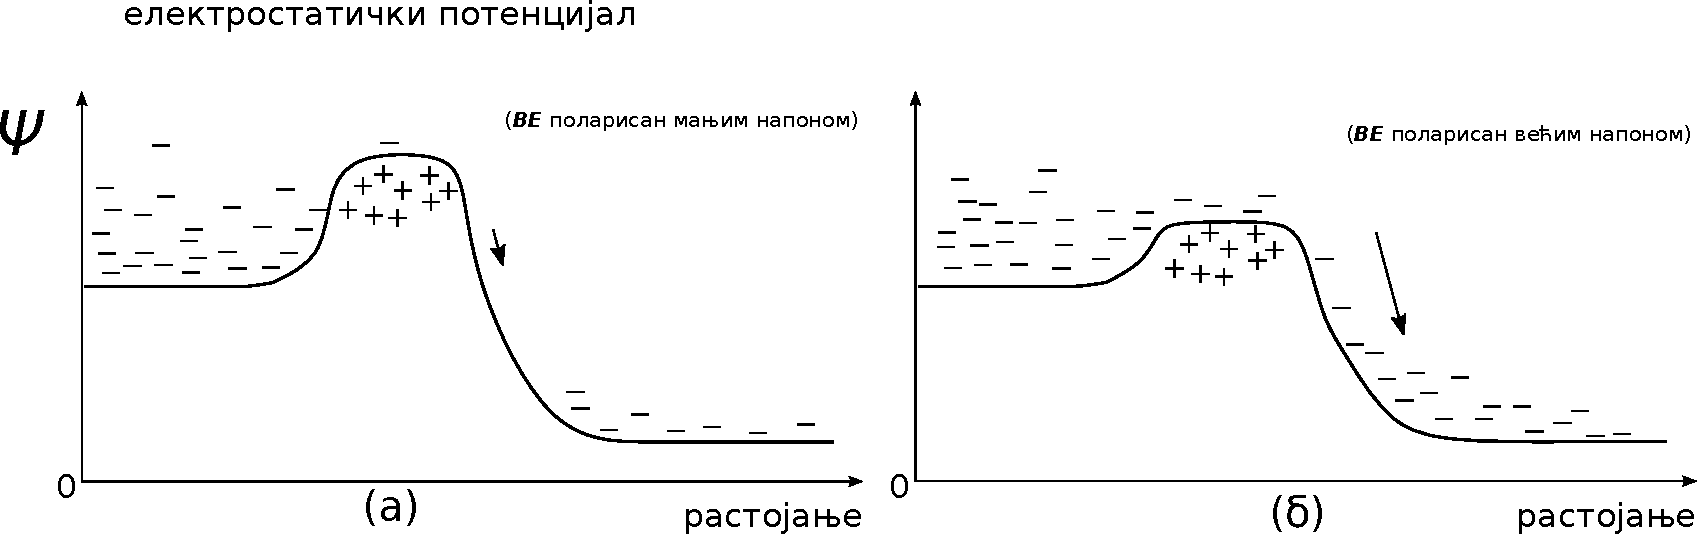
\includegraphics[width=\linewidth]{Figures/potential-energy-n-p-n-2-forward-biases.pdf}
	\caption{Потенцијална енергија електрона у \textit{n-p-n} биполарном транзистору за две вредности поларизације преко емитерског споја. (б) директна поларизација је већа него у (а)}
	\label{fig:potential-energy-n-p-n-2-forward-biases}
\end{figure}

Из гледишта електрона ситуација у транзистору који ради је приказана на слици \ref{fig:potential-energy-n-p-n-2-forward-biases}. Овај дијаграм показује варијацију у потенцијалној енергији електрона дуж линије од емитер ка колектору у транзистору који је поларисан као што је приказано у \ref{fig:structure-junction-transistor}. Обрнута поларизација на колектором споју прави велики пад у потенцијалу  са десне стране. Променљива поларизација на емитерском споју мења висину брда и тако мења дифузиону струју електрона у базу. База је веома танка и садржи веома мало \textit{deathnium}-а. Као последица вероватноће је много већа да електрон прође дифузијом кроз базу о појави се на колекторском споју него да се споји са шупљином у близини неког \textit{deathnium}-а унутар базе. Унутар добро направљеног биполарног транзистора, у ствари ток електрона кроз базу до колектора може да превазилази струју комбинације инјектоване у базни слој фактором од 100 или више. Ово значи да улазне струје контролишу 100 пута већу струју која тече у колекторски регион. Иако ова ситуације није ни близу идеалне у вакуумској триоди, у којој струја мреже је и даље мања него струја аноде, дозвољава биполарном транзистору да ради као веома ефикасан појачавач.

Биполарни транзистор има скоро идеалну пентодну карактеристику у виду колекторске сатурације. Из овога следе иста разматрања који раде добро и за ниске колекторске напона. У ствари, у неким биполарним транзисторима постоји и занемарљива варијација у струји преко напонског опсега и до 100 пута већег или још више, рецимо \SI{100}{\milli\volt} до \SI{10}{\volt} на колектору. 

Биполарни транзистор описан сликама \ref{fig:structure-junction-transistor} и \ref{fig:potential-energy-n-p-n-2-forward-biases} је само један у великој породици транзистора. Транзистори \textit{p-n-i-p} и \textit{n-p-i-n} су варијације овог облика специјално дизајниране за мале капацитивности између колектора и базе. Такозване биполарне тетроде је специјалан облик биполараца у којима струја је контролисана само малим делом региона базе. Биполарни транзистори овог типа могу да се користе као осцилаторна кола на учестаностима високим и до \SI{1000}{\mega\hertz}. На крају овог дела рада, треба нагласити да биполарни транзистор пружа више флексибилности у смислу снаге него електронске цеви. Ово је од великог значаја, пошто значи да биполарни транзистори могу да се користе ефикасно у неким случајевима где снага нивоа који треба даа се појача је много мања од струје грејања у најефикаснијим електронским цевима. Могућност рада са малим снагама је због ниских напона који су потребни за рад биполарног транзистора и због своје мале величине и могућег малог присуства нечистоћа струја услед генерације код \textit{deathnium} центара може бити мања од \SI{1}{\micro\ampere}. Због тога је могуће направити биполарни транзистор који може имати дејство појачавача са улазног снагом далеко мањом од  \SI{1}{\micro\watt}. Исти транзистор, може да ради и са високим напонима до \SI{10}{\volt} и струјама реда \SI{10}{\milli\ampere}. Може да покрије ефективни опсег од 100000. Ова чињеница показује да ће вероватно постојати мањи диверзитет типова транзистора, него што је то случај код електронских цеви.


\subsection{Закључак}

У лекцији разумног обима, није више могуће посветити се многим гранама полупроводничке физике која се развија од открића транзисторског ефекта. У претходним деловима илустрована је побуда покушаја остваривања практичних циљева која је довела до експерименталног програма, који је донео много нових и важних видова електронских феномена у полупроводницима.

Нису сва значајна истраживања, наравно, била мотивисана веома практичним циљевима која се могу одмах остварити када се фундаментална наука разуме. Већина рада на површинским стањима би требало да се посматра као чиста наука јер није могуће видети уопште како научни резултати могу наћи употребну. Ипак, веома је могуће да када се феномен површинских стања потпуно разуме из научног гледишта, многи корисни предлози ће настати на томе како се ово знање може искористити за боље уређаје.

Такође у групи чисто научних радове су лепе одреднице енергетских нивоа структуре у силикону и германијуму да резултују у циклотронској резонанци у силикону и германијуму. Овај рад је водио ка детаљнијем познавању енергетских нивоа површине него икада пре, осим можда за најједноставније и тривијалне случајеве.

Једна од највећих области која је почела да расте као резултат транзисторске технологије се може назвати "Теорија чврстих раствора унутар силикона и германијума". Скоро, интеракције између донора и акцептора различитих типова су разматране. Очигледно је интересантан феномен повезан са убацивањем било ког страног елемента из периодног система у силикон и германијум. Битне разлике су изражене за атоме у супстиционој позицији и у међупростору. Такође је откривено да неки атоми постоје у полупроводнику у не само два стања наелектрисања у случају простог донора или акцептора већ у 4 различита случаја наелектрисања. Веома је вероватно да таква област раде ће постати активна тема у физичкој хемији у наредним годинама.

Међу феноменима мотивисаним у значајној мери практичним циљевима требало би да поменемо појаву лавинског пробоја (\textit{avalanche breakdown}) које је користно у диодама које ограничавају напон и заштитним уређајиума. Јака мотривација за праћење раних назнака које предлажу да се овакви ефекти дешавају, долази од др О. Е. Баклија који поменуо пре овог предавања. Др Бакли је нагласио потребу за уређајем који штити телефоне од штете услед напона створених од муња у близини телефонских линија. У великој мери моје знање о овојх потреби је дало нагласак овом раду. Оригинална интерпретација за коју се испоставило да је сагласна са механизмом пробоја диелектрика предложена од Ценера (директно пуцање веза електронских парова јаким електричним пољем са  резулататом стварања парова електрона и шупљина) се чини као погрешна. Истраживање истог феномена од стране Мкеја и његових сарадника је довела до нове гране полупроводничке електронике која се бави утицајем јонизација шупљина на кретање електрона у јаким електричним пољима полупроводника. И ефекат и његова теорија играју активну улогу у одређеним класама прекидачких транзистора.

У завршавању овог предавања, желео бих да упутим на одломак написан у књизи 1950 године. Драго ми је да видим да су се предвиђања у овом одломку испунила у значајној мери и осећам да исто важе сада као и тада:

"Можда би било прикладно спекулисати у овом тренутку о будућности транзисторске електронике. Они који су радили интензивно у области деле ауторова осећања великог оптимизма у односу на крајње потенцијалност. Изгледа да се многим радницима у овој области отворила нова област слична целој области електронских цеви и електроника гасног пражњења. Већ је неколико транзисторских структура развијено и многи други су истражени у мери представљања њихове крајње практичности, и још других идеја је произашло, које би тек требало да буду подвргнуте адекватним експериментима. Делује вероватно да многа открића која нису предвиђена у овом тренутку ће бити заснована на принципима инјекција носиоца, утицаја поља, Золовог ефекта (\textit{Harry Suhl}) и особинама исправљачких спојева. Веома је вероватно да ће други физички принципи такође бити коришћени зарад практичном циља док се вештина развија."

\section{Површинске особине полупроводника- Братенов лауреат}



\section{Додатни материјали}
% \section{Електроника 1 - Славољуб Марјановић} није довољно добра

Тотална струја електрона се добија сабирањем струје услед дифузије и струје услед утицаја електричног поља. За електроне:

\begin{equation} \label{fig:total-current-density-electrons}
	J_n = qn \mu_n E + q D_n \dv{n}{x}
\end{equation}

слично је за шупљине:


\begin{equation} \label{fig:total-current-density-holes}
	J_p = qp \mu_p E - q D_p \dv{p}{x}
\end{equation}	


Тотална струја је сума густине струја електрона и шупљина помножена површином А, која је под правим углом у односу на смер тока струје:

\begin{equation*}
	I_{total} = A(J_n + J_p)
\end{equation*}

\subsection{Једначина континуитета}

% Једначина континуитета постоји и у теорији флуида и цеви?

\href{https://truenano.com/PSD20/contents/contents.htm}{Садржај књиге} \textit{Principles of Semiconductor Devices - B. Van Zeghbroeck}

\subsubsection{Извођење}

Једначина континуитета опсијуе једноставан концепт, да наелектрисање у концентрацији носилаца у току времена је услед разлике у долазећем и одлазећем флуксу носиоца плус генерација минус рекомбинација. Ток носиоца, стопе рекомбинације и комбинације су приказане на слици \ref{fig:discontinuity-equation-illu}:

\begin{figure}[ht!]
    \centering
	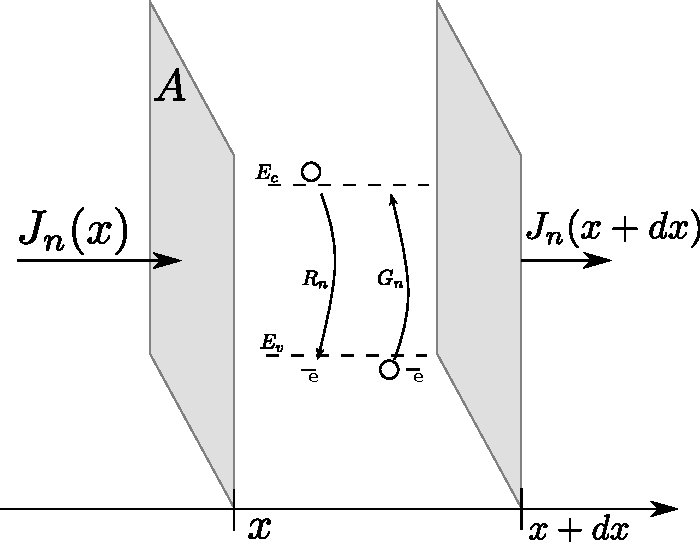
\includegraphics[width=0.6\linewidth]{Figures/discontinuity-equation-illu.pdf}
	\caption{Струје електрона и могући процеси рекомбинације и генерације}
	\label{fig:discontinuity-equation-illu}
\end{figure}


Стопа промене носиоца измећу $x$ и $x + \dd{x}$ је једнака разлици имеђу долазећег флукса и одлазећег флукса плус  генерација и минус регенерација:


\begin{equation*}
	\pdv{n(x,t)}{t} A \dd{x}  =( \dfrac{J_n(x)}{-q} - \dfrac{J_n(x + \dd{x})}{-q}) A+ (G_n(x,t) - R_n(x,t)) A \dd{x}
\end{equation*}

где су $n(x,t)$ концентрација носилаца, $A$ је површина, $G_n$ стопа генерације и $R_n $стопа рекомбинације. Користећи Тејлоров развој;

\begin{equation*}
	J_n(x + \dd{x}) = J_n(x) + \dv{J_n(x)}{x} \dd{x}
\end{equation*}

Можемо заменити $\dfrac{J_n(x)}{-q} - \dfrac{J_n(x + \dd{x})}{-q}$ диференцијалом, а површина $A$ се скрати:

\begin{equation*}
	\pdv{n(x,t)}{t} \dd{x}  = \dfrac{1}{q} \dv{J_n(x)}{x} \dd{x}  + (G_n(x,t) - R_n(x,t)) \dd{x}
\end{equation*}

слично је и за шупљине:

\begin{equation*}
	\pdv{p(x,t)}{t} \dd{x}  = - \dfrac{1}{q} \dv{J_p(x)}{x} \dd{x}  + (G_p(x,t) - R_p(x,t)) \dd{x}
\end{equation*}

Када заменимо \ref{fig:total-current-density-electrons} и \ref{fig:total-current-density-holes} у одговарајуће једначине и тиме добијамо парцијалне диференцијалне једначине у функцији концентрације електрона, концентрације шупљина и електричног поља. Електрично поље добија из Гаусовог закона:

\begin{equation*}
	\pdv{n(x,t)}{t} \dd{x}  = \dfrac{1}{q} \pdv{(qn \mu_n E + q D_n \pdv{n}{x})}{x} \dd{x}  + (G_n(x,t) - R_n(x,t)) \dd{x}
\end{equation*}

\begin{equation*}
	\pdv{p(x,t)}{t} \dd{x}  = - \dfrac{1}{q} \pdv{(qp \mu_p E - q D_p \pdv{p}{x})}{x} \dd{x}  + (G_p(x,t) - R_p(x,t)) \dd{x}
\end{equation*}

% у општем случају електрично поље се мења у простору

\begin{equation*}
	\pdv{n(x,t)}{t}  = \mu_n E \pdv{n}{x} + \mu_n n \pdv{E}{x}  +  D_n \frac{\partial^2 n}{\partial x^2}   + (G_n(x,t) - R_n(x,t))
\end{equation*}

\begin{equation*}
	\pdv{p(x,t)}{t}   = - \mu_p E \pdv{p}{x} - \mu_p p \pdv{E}{x} + D_p \frac{\partial^2 p}{\partial x^2}  + (G_p(x,t) - R_p(x,t))
\end{equation*}

Уопштена тродимензионална формула даје једначине континуитета за електорне и шупљине.

\begin{equation*}
	\pdv{n(x,y,z,t)}{t}   = \dfrac{1}{q} \vec{\nabla} \dv{\vec{J}_n(x)}{x}  + (G_n(x,t) - R_n(x,t)) 
\end{equation*}

\begin{equation*}
	\pdv{p(x,y,z,t)}{t}   = -\dfrac{1}{q} \vec{\nabla} \dv{\vec{J}_p(x)}{x}   + (G_p(x,t) - R_p(x,t)) 
\end{equation*}


% Figure 2.9.1 :	Electron currents and possible recombination and generation processes

% The rate of change of the carriers between x and x + dx equals the difference between the incoming flux and the outgoing flux plus the generation and minus the recombination:
% 	(2.9.1)

% where n(x,t) is the carrier density, A is the area, Gn(x,t) is the generation rate and Rn(x,t) is the recombination rate. Using a Taylor series expansion,
% 	(2.9.2)

% this equation can be formulated as a function of the derivative of the current:
% 	(2.9.3)

% and similarly for holes one finds:
% 	(2.9.4)

% A solution to these equations can be obtained by substituting the expression for the electron and hole current, (2.7.31) and (2.7.32). This then yields two partial differential equations as a function of the electron density, the hole density and the electric field. The electric field itself is obtained from GaussÕs law.
% 	(2.9.5)
% 	(2.9.6)

% A generalization in three dimensions yields the following continuity equations for electrons and holes:
% 	(2.9.7)
% 	(2.9.8)
\subsubsection{Једначина дифузије}

У квазинеутралном региону Đ, који садржи покретне носиоце, где је електрично поље мало - струја настаје услед само дифузије. Додатно можемо користити једноставни рекомбинациони модел за нето стопу рекомбинације пошто брзина рекомбинације зависи само од густине мањинских носилаца. Ово води ка једначинама зависним од дифузије за електроне у материјалу \textit{p}-типа и шупљина у материјалу \textit{n}-типа.

\begin{equation*}
	\pdv{n(x,t)}{t}  = D_n \frac{\partial^2 n_p}{\partial x^2}   + \dfrac{n_p(x,t) - n_{p0}}{\tau_n}
\end{equation*}

\begin{equation*}
	\pdv{p(x,t)}{t}  = D_n \frac{\partial^2 p_n}{\partial x^2}   + \dfrac{p_n(x,t) - p_{n0}}{\tau_p}
\end{equation*} % само мањински носиоци, за регенерацију и комбинацију се користи нека временска константа тау 


\subsubsection{Steady State решење диференцијалне једначине}

У \textit{steady state}-у или стабилном стању, парцијални изводи у односу на на време су једнаки 0, чиме добијамо:

\begin{equation*}
	0 = D_n \frac{\partial^2 n_p}{\partial x^2}   + \dfrac{n_p(x,t) - n_{p0}}{\tau_n}
\end{equation*}

\begin{equation*}
	0  = D_n \frac{\partial^2 p_n}{\partial x^2}   + \dfrac{p_n(x,t) - p_{n0}}{\tau_p}
\end{equation*}

Опште решење за диференцијалне једначине другог реда је:

\begin{equation*}
	n_p (x \le -x_p) = n_{p0} + C e^{\dfrac{-(x+x_p)}{L_n}} + D e^{\dfrac{-(x+x_p)}{L_n}}
\end{equation*}

\begin{equation*}
	p_n (x \ge x_n) = p_{n0} + A e^{\dfrac{-(x-x_n)}{L_p}} + B e^{\dfrac{-(x-x_n)}{L_p}}
\end{equation*}

где су $L_n$ и $L_p$ дифузионе дужине дефинисане као: 

\begin{equation*}
	L_n = \sqrt{D_n \tau_n}
\end{equation*}

\begin{equation*}
	L_p = \sqrt{D_p \tau_p}
\end{equation*}

Дифузионе константе $D_n$ и $D_p$ су дефинисане на основу Ајнштајнових релација:

\begin{equation*}
	D_n = \mu_n \dfrac{kT}{q} = \mu_n V_t
\end{equation*}

\begin{equation*}
	D_p =  \mu_p \dfrac{kT}{q} = \mu_p V_t
\end{equation*}

Дифузионе једначине се могу написати и као функција вишка концентрације носилаца, $\delta n$ и $\delta p$, које су у вези са тоталном концентрацијом $n$ и $p$, и концентрацијама термалног еквилибријума $n_0$ и $p_0$ : 

\begin{equation*}
	n = n_0 + \delta n
\end{equation*}

\begin{equation*}
	p = p_0 + \delta p
\end{equation*}

па добијамо диференцијалне једначиине:

\begin{equation*}
	0 =  \frac{\partial^2 (\delta n_p)}{\partial x^2} - \dfrac{ \delta n_p}{L_n^2}
\end{equation*}

\begin{equation*}
	0  = \frac{\partial^2 (\delta p_n)}{\partial x^2} - \dfrac{\delta p_n}{L_p^2}
\end{equation*} % ово је само скраћени запис, претходних диференцијалних једначина за које су већ дата решења.

Дифузиона једначина ће бити коришћења за израчунавање дифузионе струје у \textit{p-n} спојевима и биполарним транзисторима.




% \begin{equation}
% 	A \dd{x} \dv{p_n(t)}{t} q  = A \dd{x} q \dfrac{p_{n0}}{\tau_p} - A \dd{x} q \dfrac{p_n(t)}{\tau_p} 
% \end{equation}

% \begin{equation}
% 	A \dd{x} \dv{p_n(t)}{t} q  = A \dd{x} q \dfrac{p_{n0}-p_n(t)}{\tau_p}
% \end{equation}

% Развој Тејлоровог реда :
% \begin{equation}
% 	I_p (x+ \dd{x}) = I_p (x) + \pdv{I_p}{x} \dd{x} + \dots
% \end{equation}


% \begin{equation}
% 	 \pdv{I_p}{x} \dd{x} = I_p (x+ \dd{x}) - I_p (x)
% \end{equation}


\subsection{Фермијева енергија}

Фермијева $E_F$ је енергија повезана са честицом, која је у термалној равнотежи (еквилибријуму) са системом који посматрамо. Енергија је строго повезана са честицом и уопште није повезана са топлотом или радом. Ова иста величина се назива електро-хемијски потенцијал, $\mu$, у многим термодинамичким текстовима.

\subsection{Крониг-Пени модел електрона у силикону}

Унутар силикона могу се наћи покретна наелектрисања - електрони и непокретни позитивни јони. У Крониг-Пени моделу (добио назив по Ралфу Кронигу и Вилијам Пенију) непокретни позитивни јони се понашају као периодичне потенцијалне јаме (\textit{eng. potential wells}) за електроне. Овај модел помаже у одређивању термалних, електричних и магнетних особина материјала.

\subsection{Модел дрифт-дифузиони модел}

Овај модел се често користи да опише полупроводничке уређаје. Пре него што га будемо користили за анализе ових уређаја, особине поједностављеног модела ће бити овде представљене овде.


Претпоставке за овај поједностављени модел су:

 \begin{itemize}
	\item потпуна јонизација - претпоставка да су сви допанди јонизовани
	\item недегенерисани - претпоставка да је Фермијева енергија најмање $3kT$ испод/изнад границе кондукционе/валентне зоне 
	\item Стабилно стање - све променљиве су временски независне
	\item Константна температура - температура је констатна кроз уређај
 \end{itemize}

 Десет променљивих су: 

 \begin{itemize}
	\item $\rho$, концентрација наелектрисања
	\item $n$, концентрација електрона
	\item $p$, концентрација шупљина
	\item $E$, електрично поље
	\item $\psi$, потенцијал
	\item $E_i$, сопствена енергија
	\item $F_n$, квази-Ферми енергија електрона
	\item $F_p$, квази-Ферми енергија шупљина
	\item $J_n$, густина струје електрона
	\item $J_p$, густина струје шупљина
 \end{itemize}

\begin{info}
	Квази-Фермијеве енергије настају када електрони и шуљпине очигледно нису у термалном еквилибријуму једни са другима. Ово се дешава када се спољашњи напон нанесе на уређај који се посматра. Квазифермијеве енергије су представљене на основу да, иако електрони и шупљине нису у термалној равнотежи једни са другима, и даље су у термалном еквилибријуму сами са собом и могу бити описани Фермијевом енергијама које су сада различите за електроне и шупљине. Ове Фермијеве енергије се односе на електорн и шупљине квази-фермијивим енергија, $F_n$ и $F_p$. За недегенерисане концентрације могуће је наћи однос концентрација електрона и шупљина према две квазифермијеве енергије наредним једначинама:
\end{info}

\begin{equation*} 
	n = n_i e^{(F_n - E_i)/kT} = N_c e^{(F_n - E_c)/kT}
\end{equation*}

\begin{equation*} 
	p = p_i e^{(E_i - F_p)/kT} = N_v e^{(F_n - E_v)/kT}
\end{equation*}

Десет једначина:

Једначина густина наелектрисања:

\begin{equation*}
	\rho = q(p-n + N_d^+ - N_a^-)	
\end{equation*}


Једначине електрично поља и потенцијала:

\begin{equation*}
	\dv{E}{x} =  \dfrac{\rho}{\epsilon}
\end{equation*}


\begin{equation*} % phi или psi!?
	\dv{\phi}{x} = - E
\end{equation*}

сопствена енергија:

\begin{equation*} 
	\dv{E_i}{x} = q E
\end{equation*}

Једначине концентрације носилаца:

\begin{equation*} 
	n = n_i e^{(F_n - E_i)/kT}
\end{equation*}

\begin{equation*} 
	p = p_i e^{(E_i - F_p)/kT}
\end{equation*}

Једначине струје дрифта и дифузије:

\begin{equation*} 
	J_n = q n \mu_n E + q D_n \dv{n}{x} 
\end{equation*}

\begin{equation*} 
	J_p = q p \mu_p E - q D_p \dv{p}{x} 
\end{equation*}

Једначина континитета у стабилном стању са ШРХ (Шокли-Рид-Хол) рекомбинацијом:

\begin{equation*} 
	0 = \dfrac{1}{q} \pdv{J_n}{x} - \dfrac{np - n_i^2}{n + p + 2n_i cosh(\dfrac{E_t - E_i}{kT})} \dfrac{1}{\tau}
\end{equation*}
 
\begin{equation*} 
	0 = -\dfrac{1}{q} \pdv{J_p}{x} - \dfrac{np - n_i^2}{n + p + 2n_i cosh(\dfrac{E_t - E_i}{kT})} \dfrac{1}{\tau}
\end{equation*}


% Abstract from \href{https://ieeexplore.ieee.org/document/4456783}{Fully Integrated CMOS Power Amplifier With Efficiency Enhancement at Power Back-Off}, Gang Liu, Peter Haldi, Tsu-Jae King Liu, Fellow, IEEE, and Ali M. Niknejad, Member, IEEE

% \begin{info}
% 	\textbf{Abstract} — This paper presents a new approach for power amplifier design using deep submicron CMOS technologies. A transformer based voltage combiner is proposed to combine power generated from several low-voltage CMOS amplifiers. Unlike other voltage combining transformers, the architecture presented in this paper provides greater flexibility to access and control the individual amplifiers in a voltage combined amplifier. In this work this voltage combining transformer has been utilized to control output power and improve average efficiency at power back-off. This technique does not degrade instantaneous efficiency at peak power and maintains voltage gain with power back-off. A 1.2 V, 2.4 GHz fully integrated CMOS power amplifier prototype was implemented with thin-oxide transistors in a 0.13 m RF-CMOS process to demonstrate the concept. Neither off-chip components nor bondwires are used for output matching. The power amplifier transmits 24 dBm power with 25\% drain efficiency at 1 dB compression point. When driven into saturation, it transmits 27 dBm peak power with 32\% drain efficiency. At power back-off, efficiency is greatly improved in the prototype which employs average efficiency enhancement circuitry.
% \end{info}

% % why does this transformer have greater flexibility

% % neither the off-chip components nor bondwires are used for output matching

% The cascode gate is connected to the supply node when the individual amplifier is on, and it is grounded to turn off the individual amplifier for power back-off (to improve PAE when the output power is backed off).\\


% Abstract from \href{https://ieeexplore.ieee.org/document/4494655}{A 5.8 GHz 1 V Linear Power Amplifier Using a Novel On-Chip Transformer Power Combiner in Standard 90 nm CMOS}

% \begin{info}
% 	\textbf{Abstract} — A fully integrated 5.8 GHz Class AB linear power amplifier (PA) in a standard 90 nm CMOS process using thin oxide transistors utilizes a novel on-chip transformer power combining network. The transformer combines the power of four push-pull stages with low insertion loss over the bandwidth of interest and is compatible with standard CMOS process without any additional analog or RF enhancements. With a 1 V power supply, the PA achieves 24.3 dBm maximum output power at a peak drain efficiency of 27\% and 20.5 dBm output power at the 1 dB compression point
% \end{info}

% % It does not mention the broadband matching circuits

% % https://sci-hub.se/10.1007/s11432-016-0299-4

% % https://sci-hub.se/10.1109/RWS.2014.6830155 

% % PAE is closely connected to operating frequency of power amplifier.

% %====================================================================================================================================================================================
% \section{Conversation about design}
% %====================================================================================================================================================================================

% You were talking about previous design and also about need to do redesign. What exact parameters you did not match last time, and do you have also starting design and schematic ready, or you would like to ask us to start completely form beginning?

% \textcolor{blue}{[John]: Compared with current design, we would lower the PA output power from max 16dBm to 0dBm, and reduce the PA area as much as possible. We would like to redesign the existing PA because the current design is silicon proven and we have delivered more than 1 million pcs. And we have a redesign strategy in our mind. We can discuss it in the intake meeting.}

% I am guessing that we are doing also design and layout due to the fact that it is a RF component?

% \textcolor{blue}{[John]:  yes, that is the plan that  you redesign PA and do the layout. We will integrate to the SoC }

% I am guessing this component will be further integrated in the complex SOC? 

% \textcolor{blue}{[John]: yes, it will be integrated into WiFi SoC. }

% Do you have power control of PA?  If yes do you have other specs? 

% \textcolor{blue}{[John]: yes, we can propose other specs. However, we would purposely only define the most important specs(EVM, OIP3, VDD, Freq, BW, process technology ) in our design request because we would give the freedom to the PA designer as much as we can. We can discuss  in the intake meeting. }

% Do you have any special circutry like power detector to measure if antenna is working (connection ok), or the whole power is reflected back. Self performance test.

% \textcolor{blue}{[John]: No, power detector isn't included in this PA redesign work.  } 

% Are those parameters down only one for acceptance criteria?

% \textcolor{blue}{[John]: They are the key specs. We definitely need more items as acceptance criteria, but we are open to define together with PA design team to give freedom to the PA to make a better trade-off.  }

% You were talking about size? What size you have currently?

% \textcolor{blue}{[John]: One PA block consists of four identical units. each unit is about 0.13mm2. so for one PA, it is about 0.52mm2.   }

% I am guessing we are using our Cadence tools, and simulators?

% \textcolor{blue}{[John]: It depends on availability of the CAD tool\&PDK version, the cost and the team preference. we can also align in the intake meeting.} 



% % Min and max for supply voltage are not defined in the original document, and time for switching between two cores was defined during the meeting. Updated 2* specification for phase noise, frequency pushing update not clear.

% % Currently Full LO range is split between two cores so the requirement should look like this:

% % \begin{table}[ht]
% % 	\centering
% % 	\begin{tabular}{|c|l|c|c|c|c|c|}
% % 		\hline
% % 		& LO range requirements & Note & min & typ & max & Units \\
% % 		\hline
% % 		1 & High Band core LO range &  & 10000  &  & 13700 & MHz \\ 
% % 		\hline
% % 		2 & Low Band core LO range &  & 6300 &  & 10000 & MHz \\ 
% % 		\hline
% 	\end{tabular}
% 	\caption{LO Range Two Core Specification Requirements} 
% \end{table}

% \begin{question}[\itshape What's the variation for supply voltage?]
% 	Not defined probably will be the same as the rest of the 
% \end{question}


% \begin{question}[\itshape $K_{VCO}$ Why is it in the max column? ]
% 	Didn't get answer for this. It's probably also typical and a value that is expected by the PLL design.
% \end{question}

% % Footnotes do not work.

% Process corners can be found at:

% \begin{verbatim}
% /tech/tsmc/tsmc40/models/spectre/crn40lp_2d5_v2d0_2_shrink0d9_embedded_usage.scs
% \end{verbatim}
% % Seems that 

% \section{Scaldio Design Review}

% \begin{question}[\itshape How should calibration be implemented to achieve output voltage peak to peak and minimize noise?]
% Is it done for whole PLL?
% \end{question}

% \begin{question}[\itshape Difference between class-B and class-C vco? ]
% 	Scaldio uses class-C, so all parasitic capacitances connected to the tail don't matter. Having trouble with observing the currents of drain so cannot check this and compare them. Scaldio looks something between class C and class B because of $V_{gbias}$ voltage and because adding inductor between tail NMOS and switching pair improves phase noise. This is attributed to class B, while class C only needs tail capacitance.
% \end{question}






% \begin{figure}[ht!]
% 	\centering
% 	\includegraphics[width=0.7\linewidth]{Figures/class-B_vs_class-C.pdf}
% 	\caption{Schematic difference between class C and class B}
% 	\label{fig:classC_classB_inkscape}
% \end{figure}


% Lowest bit of digital varactor (L0\_PLL\_hbVCO\_Cdig\_SC2B\_VCOS\_SC2C\_PLL) doesn't do anything, isn't even monotonous. Maybe makes more sense when simulating extracted cells. Digital varactor needs to be redesigned, it could lower the Q factor.
% Main difference between class B and class C can be observed by investigating their drain currents.

% \begin{figure}[ht!]
% 	\includegraphics[width=\linewidth]{Figures/drainCurrent_classB_vs_classC.png}
% 	% \caption{Difference between class C and class B}
% 	\label{fig:drainCurrent_classB_vs_classC}
% \end{figure}

% \subsection{Main testbench}

% Main testbench covers everything except for frequency pulling and full LO range. The simulation results are obtained at the higher end of the LO range. Phase noise is simulated by pss+pnoise.

% \begin{info} % Information block
% 	With Noise Type=timeaverage and ALL(AM,PM,USB,LSB), you can plot the AM and PM components as well as the total noise. In addition, you can plot phase noise and FM jitter results for oscillators. Plotting is done using the Direct Plot Form.
% 	\href{https://community.cadence.com/cadence_blogs_8/b/rf/posts/virtuoso-video-diary-noise-simulation-in-spectre-rf-using-improved-pnoise-hbnoise-and-direct-plot-form-options}{\textbf{External link}}
% \end{info}

% Function of phase noise is simulated for PM noise type.

% How to choose beat frequency for autonomous system from forum \href{https://community.cadence.com/cadence_technology_forums/f/custom-ic-design/2661/beat-frequency-in-spectrerf-pss-simulation}{\textbf{thread}}.

% \begin{info} % Information block
% In an autonomous system (e.g. an oscillator), you turn on the "oscillator" checkbox, and the beat frequency is then the estimated frequency, which gives PSS a starting point to solve for the oscillator frequency. It's important when in oscillator mode to select the outputs of the circuit, which include any subharmonics. In other words, if you have an oscillator followed by a divider, point at the divider output, and give the estimated divided frequency as the beat frequency. Again, this is because you need to solve an integer number of cycles of all the frequencies in the circuit. Note, don't use oscillator mode for circuits which aren't oscillators, since you're then trying to get the simulator to solve for an unknown which is not unknown, which may lead to convergence problems.
% \end{info}

% Most of the $I_{bias}$ tune digital control is not used for the higher band, so by increasing the number of steps to cover even higher frequencies than the original design finer bias control is needed.


% \subsection{Simulation Results for Scaldio design}

% Simulated only nominal corner with change for $V_{DD}$ only for frequency pushing simulation. 

% \begin{table}[ht]
% 	\centering
% 	\begin{tabular}{|c|l|c|c|c|c|c|c|}
% 		\hline
% 		& LO Requirements & Note & min & typ & max & Sim(Typ) & Units \\
% 		% \hline
% 		% & \multicolumn{7}{|c|}{VCO Requirements} \\
% 		\hline
% 		1 & Phase Noise at 300 kHz &  &  &  & <-101 & -98 & dBc/Hz  \\ 
% 		\hline
% 		2 & Tuning Sensitivity $K_{VCO}$ &  &  &  & 100 & over & MHz/V  \\ 
% 		\hline
% 		3 & Pushing & TBD &  &  & 2  & 279.7 & MHz/V  \\ 
% 		\hline
% 		4 & Output Voltage & TBD & 800 &  & & 809.3 & $mV_{p-p}$  \\ 
% 		\hline
% 		5 & Harmonic suppression ($2_{nd}$, typ) &  & -15 &  & & -26.78 & dBc  \\ 
% 		\hline
% 		6 & Pulling (14 dB Return Loss, Any Phase) & TBD &  &  & 2  & 19.51 & MHz  \\ 
% 		\hline
% 	\end{tabular}
% 	\label{table-ScaldioResults}
% 	\caption{Scaldio IMEC design Results}
% \end{table}

% Phase noise changes a lot for different tuning voltages between -90 and -100 dBc/Hz. Phase noise is probably not modeled ok because the VCO doesn't have the connection between current bias tail and the switching pair of VCO as transmission line. That inductance and $C_{tail}$ should resonate at 2$\omega_O$ (tank oscillating frequency), but only in the case of class B oscillator. Check what type is vco oscillator. %This is hard to check because pss\_tran drain currents look wierd.

% \newpage

% %----------------------------------------------------------------------------------------
% \section{Q factor of LC tank}

% Need testbenches capacitance of tank, varactors and inductor, and for different controls and also corners. Process corners for varactors are the same as MOSFET.

% % and of tail (to see how to make it resonate at the double of the oscillating frequency).

% \begin{question}[\itshape What kind of chip is it?]
% 	What kind of inductance is expected to be connected on $V_{DD}$ and $V_{SS}$ pins. This may or may not change the results. Removed all together right now.
% \end{question}

% Testbench for differential Q and L of the inductor that is EMX simulated is shown in Figure \ref{fig:qlinductor}.

% \begin{figure}[ht!]
% 	\includegraphics[width=\linewidth]{Figures/QL_inductor.png}
% 	\caption{Q factor and inductance of L}
% 	\label{fig:qlinductor}
% \end{figure}

% Q factor is better at the higher frequency.

% Simulated Q factor of both varactors and inductor. Q factor of digital varactor for lower bit controls is not much better than Q of inductor.

% Capacitor calculating capacitance and Q factor:

% \begin{equation}
% 	Y_{diff} (im) = imag(ypm('sp 1 1)) + imag(ypm('sp 2 2)) - imag(ypm('sp 2 1)) - imag(ypm('sp 1 2))
% \end{equation}

% \begin{equation}
% 	Y_{diff} (re) = real(ypm('sp 1 1)) + real(ypm('sp 2 2)) - real(ypm('sp 2 1)) - real(ypm('sp 1 2))
% \end{equation}

% Capacitance:
% \begin{equation}
% 	C_{diff} = \dfrac{Y_{diff} (im)}{2\pi f}
% \end{equation}

% Q factor of capacitor:
% \begin{equation}
% 	Q_C = \dfrac{Y_{diff} (im)}{ Y_{diff} (re)}
% \end{equation}

% \begin{figure}[h!]
% 	\includegraphics[width=\linewidth]{Figures/Dvaractor.png}
% 	\caption{C and Q of digital varactor through controls}
% 	\label{fig:dvaracator}
% \end{figure}

% More info can be found in  \href{https://ieeexplore.ieee.org/abstract/document/5537949}{\textbf{paper }} A Thorough Analysis of the Tank Quality Factor in LC Oscillators with Switched Capacitor Banks.

% How to calculate Q factor of tank from the same paper.

% \begin{info}
% It can be proved (and it is a well known result) that the quality factor of the tank is equal to the parallel combination of the quality factor of the inductance, $Q_L$, and the quality factor of the capacitance, $Q_C$ , that make up the resonant circuit. Once we have the two quality factors $Q_L$ and $Q_C$ is hence very easy to calculate $Q_T$ .
% \end{info}


% Found definitions:

% \begin{equation}
% 	Q_{LC} = \dfrac{1}{R}\sqrt{\dfrac{L}{C}} = \frac{f_r}{\Delta f} = \frac{\omega _r}{\Delta \omega} = \dfrac{\tau _d \omega}{2}
% \end{equation}

% where $\tau _d$ is group delay. Also


% \begin{equation}
% 	Q_{T} = Q_{LC} = \omega \dfrac{ES}{APD}
% \end{equation}

% where ES is energy stored and APD is average power dissipation.

% \begin{question}[\itshape How to calculate group delay using sparam analyis?]
% 	?
% \end{question}

% \subsection{Calculating Q factor‚ LC tank by ringing method}

% Link to \href{https://www.giangrandi.ch/electronics/ringdownq/ringdownq.shtml}{\textbf{website}} that shows ring down method of calculating Q factor. Not implemented in virtuoso TODO.


% %----------------------------------------------------------------------------------------
% \section{Figure of Merit different definitions}

% \begin{info} % Information block
% 	The theoretical maxima for the FoM of an oscillator is given by $FoM=174+20log_{10}(Q)$ dBc/Hz
% \end{info}

% How to calculate oscillator FoM? Is $Q_L$ factor dominant enough to just equate it with LC tank Q facor.

% The widely used FOM is calculated by:
% \begin{equation}
% 	FoM = L\{ \Delta \omega \}( \Delta f/f_0)^2 PVCO [mW]
% \end{equation}

% Where $L\{\Delta \omega\}$ is the phase noise, $ \Delta \frac{f}{f_0}$ is the ratio between the offset frequency and the carrier, and $P_{VCO}$ is the power consumption of the VCO-core. There is also $FoM^T$ and $FoM_A$ 

% \begin{equation}
% 	FoM^T = FoM - 20 \log (\dfrac{FTR}{10})
% \end{equation}

% and 

% \begin{equation}
% 	FoM_A = FoM + 10 \log (A)
% \end{equation}

% where A is area [$mm^2$], and FTR frequency tuning range [$\%$]

% Information about digital varactor copied from \href{https://www.doe.carleton.ca/~ddchen/Tutorials/DCO.pdf}{\textbf{External link}}

% \begin{info} % Information block
% Each bit of MIM varactor contains two MIM capacitors connected differentially with a series switch, two pull-up and two pull-down transistors to effectively turn the varactor between its high and low-capacitance states. Measured intrinsic Q of the MIM capacitor is 80 at 3.6 GHz. When is turned on, i.e., high-capacitance state, the varactor Q drops to 30. When is turned off to be in low-capacitance state, the parasitic capacitance of the MIM capacitor and transistors has an effective of 50. The pull-down transistors set the DC levels for drain and source of at 0 V so that
% can be efficiently turned into triode region while the weak pull-up transistors set the DC level to VDDOSC to reduce the parasitic capacitance of thus increasing of the parasitic capacitance. The pull-up pMOS can be implemented by either resistors or transistors. The latter was chosen for silicon area efficiency. Compared to MOS varactors, MIM varactors have a much lower . However, since the differential phase-stability inductor is only 10, the impact of lower varactor is tol erable. When the MIM varactor is at its low-capacitance state, the large DCO internal signal swing and the DC level of 1.4-V supply voltage at source/drain of the pull-up transistors force the drain -nwell junction diodes of the pull-up pMOS to momentarily go into forward-bias condition resulting in a latch-up concern. However, since the forward-bias condition occurs only in 50\% of a 3–4 GHz period, the latch-up phenomenon with the parasitic BJTs can not be triggered.
% \end{info}

% %----------------------------------------------------------------------------------------
% \section{Lowering frequency pushing and LDO}

% About Frequency pushing from \href{https://www.atlantis-press.com/article/6376.pdf}{\textbf{this paper}}

% \begin{info} % Information block
% An LC-tank VCO circuit has been implemented in a standard 0.35 $\mu m$ CMOS technology. It is based on a two-transistor biasing structure that improves the performance of frequency pushing and frequency tuning range. Final measurement of proposed structure gives 516 MHz tuning range with 2.278 GHz center frequency and about 0.55$\%$/V frequency pushing in the worst case. The achieved FOM is about -180dBc/Hz, which is very close to the simulated value. This structure is proven to be particularly suitable for achieving low FOM in the VCO circuits having low Q factor LC-tank. Both, the proposed structure and the FOM optimization method, can also be applied to the VCO designs for the applications at higher frequencies, such as 5GHz VCOs for Wireless LAN applications.
% \end{info}

% \begin{question}[\itshape Can VCO work for lower voltage of 0.9 V?]
% 	This may be needed if LDO is required because of frequency pushing?
% \end{question}

% \begin{question}[\itshape Does frequency only happen because of the ripple directly induced by buffers e.g.?]
% 	Or could it happen because of EM crosstalk?
% \end{question}


% Is frequency pushing testbench good? Look into this paper. % which paper
% Different testbench would be to make a transient change in Vdd and check how much frequency changes.


% Results for class C with pmos bias, only dc change of $V_{DD}$:

% \begin{center}
% 	\begin{tabular}{|l|c|c|c|c|c|c|c|c|c|}
% 		\hline
% 		Parameter & typical & spec  & min & max & ss -40 & ss 125 & ff -40 & ff 125 & Units \\
% 		% \hline
% 		% & \multicolumn{7}{|c|}{VCO Requirements} \\
% 		\hline
% 		Frequency Pushing & 43.93 & < 2 &  43.93 & 100.1 & 100.1 & 64.36 & 75.48 & 64.09 & MHz \\ 
% 		\hline
% 		Frequency  & 14.6 & > 14.2  & 14.6 & 15.83 & 15.54 & 15.48 & 15.83 & 15.59 & GHz  \\ 
% 		\hline
% 	\end{tabular}
% \end{center}

% This shows some improvement from frequency pushing of 250 - 300 MHz that was observed for the NMOS bias of IMEC Scaldio design.

% %----------------------------------------------------------------------------------------
% \section{Changing topology and lowering phase noise}

% Decision on why is single sided oscillator chosen instead of double sided oscillator.

% \begin{info}
% However, if non-negligible parasitic capacitances are found at the tank outputs, the phase-noise performance of the DS-VCO may be seriously degraded, while that of the SS-VCO remains unaffected.
% \end{info}

% More on the $\frac{1}{f^2}$ Phase Noise Performance of CMOS Differential-Pair LC-Tank Oscillators in \href{https://backend.orbit.dtu.dk/ws/files/3913656/Andreani.pdf}{\textbf{paper}} by Pietro Andreani.


% \subsection{Hybrid class C and class B}

% \begin{info}
% Further, the proposed VCO solves the issue of the hybrid mixed-signal start-up procedure exposed in [8]. The main drawback of this approach is that, if oscillation stops for some unaccountable reason, the VCO can only be restarted actuating again the whole start-up procedure.
% \end{info}

% Referenced paper is:

% \begin{itemize}
% 	\item [8] J. Chen, F. Jonsson, M. Carlsson, C. Hedenas, and L.-R. Zheng, “\href{https://ieeexplore.ieee.org/document/5951800}{A low power, startup ensured and constant amplitude class-C VCO in \SI{0.18}{\micro\metre} CMOS},” IEEE Microw. Wireless Compon. Lett., vol. 21, no. 8, pp. 427–429, 2011. Dec. 2008.
% \end{itemize}


% \subsection{Enhanced Oscillation Swing}

% Class-C VCO With Amplitude Feedback Loop for Robust Start-Up and Enhanced Oscillation Swing in \href{https://ieeexplore.ieee.org/stamp/stamp.jsp?arnumber=6377236}{\textbf{this paper.}} Phase noise is lowered by lowering $V_{gbias}$, but it makes oscillations start up harder.

% \begin{info}
% As noted above, the phase noise improves with increasing the oscillation amplitude, which here would mean lowering the gate bias voltage, $V_{bias}$ . Unfortunately, the original class-C oscillator limits the fixed $V_{bias}$ from being set low enough, otherwise the oscillation may not start up. In [11], a high-swing class-C (HSCC) oscillator was introduced, which removed the tail current transistor of the original class-C oscillator [6]. Instead, an automatic amplitude control was introduced to stabilize the oscillation amplitude. In this work, instead of the transformer used in [11], we choose a simple RC bias circuit.
% \end{info}

% This is from \href{https://www.semanticscholar.org/paper/Dual-Core-High-Swing-Class-C-VCO-design-Kim-Kim/c9551af0809604f76263af49976df9efc213bb8e}{\textbf{paper}} Dual-Core High-Swing Class-C VCO design, and references 


% \begin{itemize}
% 	\item [6] A. Mazzanti and P. Andreani, “\href{https://ieeexplore.ieee.org/document/4684621}{Class-C harmonic CMOS
% 	VCOs, with a general result on phase noise},” IEEE J.
% 	Solid-State Circuits, vol. 43, no. 12, pp. 2716–2729,
% 	Dec. 2008.
% 	\item [11] M. Tohidian, A. Fotowat-Ahmadi, M. Kamarei, and F.
% 	Ndagijimana, “\href{https://ieeexplore.ieee.org/document/6045015}{High-swing class-C VCO},” in Proc.
% 	ESSCIRC, Sep. 2011, pp. 495–498
% \end{itemize}


% \subsection{Questions about new double feedback}


% Amplitude Control Feedback and Voltage bias control for Robust start up. 

% % \begin{question}[\itshape What is?]
% % 	This may be needed if LDO is required because of frequency pushing?
% % \end{question}


% \subsection{OTA1 - Start up  and gate voltage bias control}

% Referent voltage should be set and controlled around 800 mV. Need tests for OTAs inside for VCO, currently simulated only PM and DC gain, should test different $V_{ref}$ levels.

% \subsection{OTA2 - Start up and bias control}

% Referent voltage should be set and controlled around 400 mV. Problem with OTA2 loop is amplifying noise into the tail bias current. So the new problem arises as noise shaping in LOOP2 is needed. If a OTA of low uGBW is used than start up is too slow.


% %----------------------------------------------------------------------------------------
% \section{Full LO Range and Frequency Recentering}

% % TODO Setup the lb vco, and also setup different testbenches for the highest and the lowest frequency available. Add corner analysis PVT.

% TODO Add corners for \textbf{fs sf} and similar. Because the LO range is split on two cores, ideally halved. Results are simulated for process and temperature corners: 

% \begin{table}[ht]
% 	\centering
% 	\begin{tabular}{|l|c|c|c|c|c|}
% 		\hline
% 		Core and Specifictaion & min & max & sim(min) & sim(max) & Units \\
% 		\hline
% 		\multicolumn{6}{|c|}{VCO core split} \\
% 		\hline
% 		High Band Higher limit & 13700 &  & 15580 & 16190  &  MHz  \\ 
% 		\hline
% 		High Band Lower limit &  & 10000 & 10870 & 12460 &  MHz  \\ 
% 		\hline
% 		High Band range & 3700 &  & 4710 & 3730 &  MHz  \\ 
% 		\hline
% 		Low Band Higher limit & 10000 &   & 13230 & 14120 &  MHz  \\ 
% 		\hline
% 		Low Band Lower limit &  & 6300 & 6724 & 8028  &  MHz  \\ 
% 		\hline
% 		Low Band range & 3700 &  & 6506 & 6092 &  MHz  \\ 
% 		\hline
% 	\end{tabular}
% 	\caption{LO range specification and simulation for Scaldio LC tank}
% \end{table}

% Expecting the drop for schematic simulated frequency range, covered range should at least be larger than needed when recentered: 

% \begin{equation}
% 	HBFR = 13700 - 10000 = 3700 < 3730 = 16190 - 12460
% \end{equation}

% For lower band it's similarily calculated

% \begin{equation}
% 	HBFR = 10000 - 6300 = 3700 < 6092 = 14120 - 8028
% \end{equation}

% Lower and higher band are assymetrical and they overlap for at least:

% \begin{equation}
% 	HBLBoverlap_{high} = 13230 - 10870 = 2360
% \end{equation}

% \begin{equation}
% 	HBLBoverlap_{low} = 14120 - 12460 = 1660
% \end{equation}

% The worst available frequency digital controlled range is $6092 + 3730 - 1660 = 8162$ MHz which is higher than 7400 MHz.

% \begin{question}[\itshape Are the two VCO-s in the same process corner at the same time?]
% 	Yes. If not than the calculations are wrong.
% \end{question}

% NOTE: Analog varactor 0-Vt-1 change does not work so it wasn't included. Further frequency recentering after extraction will be needed.

% \subsection{Frequency Tuning Range (FTR)}

% Frequency tuning range is calculated:
% %----------------------------------------------------------------------

% UHF channel radio 380 MHz - 512 MHz. TOCHECK
% Why does it matter for the phase noise.

% %----------------------------------------------------------------------------------------
% \section{Pulling testbench and design of VCO buffer}

% Needs port at and tuning circuit to keep the reflection at -14 dB. Port of reference impedance 10 k$\Omega$ and portAdapter from rfExamples. S parameter analysis to show if the reflection really is -14 dB? Load impedance increased from 100 fF to 1000 fF. VCO buffer is also needed because of the frequency pulling. Does each core have a buffer or do they share it? first make a buffer than maybe a question.

% By adding two buffers from \verb c LO_FDDQ_v6c, \verb c LO_FDDQ_INHB_v5_JCx_scaldio2b  and \verb cLO_FDDQ_BUF_X24 c, frequency pulling drops below 1 MHz. 

% So this specification looks fine, testbench shown:

% \begin{question}[\itshape How does portAdapter work?]
% \end{question}

% Frequency pulling mentions coupling (crosstalk) between different blocks on chip and the VCO.
% %----------------------------------------------------------------------------------------
% \section{Bandgap - PTAT and CTAT, the temperature independant Vbias for cascode}

% AC noise results of the bandgap is shown in Fig. \ref{fig:ac_noise_Bandgap}.

% \begin{figure}[!ht]
% 	\includegraphics[width=\linewidth]{Figures/ac_noise_Bandgap.jpg}
% 	\caption{AC Noise result of bandgap}
% 	\label{fig:ac_noise_Bandgap}
% \end{figure}

% \ref{fig:phase_noise_Bandgap_pBias_LNeq0&1}

% \begin{figure}[!ht]
% 	\includegraphics[width=\linewidth]{Figures/phase_noise_Bandgap_pBias_LNeq0&1.jpg}
% 	\caption{Phase Noise of the Bandgap with PMOS bias when LN is set to 0 or 1}
% 	\label{fig:phase_noise_Bandgap_pBias_LNeq0&1}
% \end{figure}

% TODO Maybe add some results over PVT for Bandgap

% TODO Use this info on the original NMOS VCO Scaldio design.

% \subsection{PTAT and CTAT, the temperature independant Vbias for cascode}

% % \verb c c

% TODO Simulate and show results of temperature sweep. (probably done maybe plot)

% %----------------------------------------------------------------------------------------

% \section{Design of tail transistors}

% Tail transistors need to be designed carefully because of their effect on the phase noise performance of VCO.

% If the inductor is resonating at double the oscillation frequency with the parasitic capacitance at the common nMOS-pair source, this technique greatly reduces both and white noise from the tail bias transistor [12]. It is, however, associated with two momentous drawbacks: it is narrowband in nature

% \subsection{Effect of too high tail capacitance}

% \begin{figure}[!ht]
% 	\includegraphics[width=\linewidth]{Figures/squegging.png}
% 	\caption{Squegging}
% 	\label{fig:squegging}
% \end{figure}

% Instability Low frequency amplitude modulation squegging. This was the issue with the original class C with tail current. Is it important for new topology where current bias is PMOS.

% TODO simulate for high and for low frequency. How to simulate envelope? 


% \section{PLL theory - PLL Lock Detect and calibration}

% About PLL Lock Detect:

% \begin{info} % Information block
% 	The ability for a PLL to reliably indicate when it is in lock is critical for many applications. An ideal lock detect circuit gives a high indication when the PLL is locked and a low indication when the PLL is unlocked. When VCO calibration finishes it can be indicative if the lock is detected. 
% \end{info}

% PLL VCO calibration usually goes as amplitude frequency and then amplitude calibration, or the other way?

% Divide and Conquer algorithm is used to find the lock.

% \begin{figure}[!ht]
% 	\includegraphics[width=\linewidth]{Figures/PLL_basics_regarding_VCO.png}
% 	\caption{Gain for VCO and  other blocks inside of PLL}
% 	\label{fig:PLL_basics_regarding_VCO	}
% \end{figure}

% \begin{info}
% 	For the VCO, the noise is suppressed below the loop bandwidth frequency and unshaped above the loop bandwidth.
% \end{info}

% PLL must implement shutdown mode.

% \subsection{Definition of PLL}

% PLL is an automatic control system that adjusts the frequency /phase of the controlled voltage generator (VCO). The type of frequency division is integer (1/N) + fractional (1/224).  The PLL unit includes:  an integer unit of the reference frequency divider R, a frequency-phase detector PFD and a charge pump CP circuit, integer and fractional dividers N + F of the VCO frequency (fractional circuit controls the divider c sigma-delta modulator with programmable order from 1 to 4. The denominator of the divisor fraction has a bit depth of 24 bits), loop filter Loop Filter.

% \section{FDDQ block}

% FDDQ block is connected to the PLL and VCO output, as VCO output buffer. The block LO25 which is located close to mixers generates 25\% duty cycle.

% \begin{question}[\itshape What is considered VCO buffer ?]
% 	Whole FDDQ or just inhb and inlb?
% \end{question}





% 50 or 100 ns for the SAW filter

% differential instead of pseudo differential 

% source degeneration


% \begin{question}[\itshape What kind of output is needed ?]
% 	s
% \end{question}


% % Math equation/formula
% \begin{equation}
% 	I = \int_{a}^{b} f(x) \; \text{d}x.
% \end{equation}

% \begin{info} % Information block
% 	This is an interesting piece of information, to which the reader should pay special attention. Fusce varius orci ac magna dapibus porttitor. In tempor leo a neque bibendum sollicitudin. Nulla pretium fermentum nisi, eget sodales magna facilisis eu. Praesent aliquet nulla ut bibendum lacinia. Donec vel mauris vulputate, commodo ligula ut, egestas orci. Suspendisse commodo odio sed hendrerit lobortis. Donec finibus eros erat, vel ornare enim mattis et.
% \end{info}

% \begin{center}
% 	\begin{minipage}{0.5\linewidth} % Adjust the minipage width to accomodate for the length of algorithm lines
% 		\begin{algorithm}[H]
% 			\KwIn{$(a, b)$, two floating-point numbers}  % Algorithm inputs
% 			\KwResult{$(c, d)$, such that $a+b = c + d$} % Algorithm outputs/results
% 			\medskip
% 			\If{$\vert b\vert > \vert a\vert$}{
% 				exchange $a$ and $b$ \;
% 			}
% 			$c \leftarrow a + b$ \;
% 			$z \leftarrow c - a$ \;
% 			$d \leftarrow b - z$ \;
% 			{\bf return} $(c,d)$ \;
% 			\caption{\texttt{FastTwoSum}} % Algorithm name
% 			\label{alg:fastTwoSum}   % optional label to refer to
% 		\end{algorithm}
% 	\end{minipage}
% \end{center}

% Fusce varius orci ac magna dapibus porttitor. In tempor leo a neque bibendum sollicitudin. Nulla pretium fermentum nisi, eget sodales magna facilisis eu. Praesent aliquet nulla ut bibendum lacinia. Donec vel mauris vulputate, commodo ligula ut, egestas orci. Suspendisse commodo odio sed hendrerit lobortis. Donec finibus eros erat, vel ornare enim mattis et.

% % Numbered question, with an optional title
% \begin{question}[\itshape (with optional title)]
% 	In congue risus leo, in gravida enim viverra id. Donec eros mauris, bibendum vel dui at, tempor commodo augue. In vel lobortis lacus. Nam ornare ullamcorper mauris vel molestie. Maecenas vehicula ornare turpis, vitae fringilla orci consectetur vel. Nam pulvinar justo nec neque egestas tristique. Donec ac dolor at libero congue varius sed vitae lectus. Donec et tristique nulla, sit amet scelerisque orci. Maecenas a vestibulum lectus, vitae gravida nulla. Proin eget volutpat orci. Morbi eu aliquet turpis. Vivamus molestie urna quis tempor tristique. Proin hendrerit sem nec tempor sollicitudin.
% \end{question}


% % File contents
% \begin{file}[hello.py]
% \begin{lstlisting}[language=Python]
% #! /usr/bin/python

% import sys
% sys.stdout.write("Hello World!\n")
% \end{lstlisting}
% \end{file}

% Fusce eleifend porttitor arcu, id accumsan elit pharetra eget. Mauris luctus velit sit amet est sodales rhoncus. Donec cursus suscipit justo, sed tristique ipsum fermentum nec. Ut tortor ex, ullamcorper varius congue in, efficitur a tellus. Vivamus ut rutrum nisi. Phasellus sit amet enim efficitur, aliquam nulla id, lacinia mauris. Quisque viverra libero ac magna maximus efficitur. Interdum et malesuada fames ac ante ipsum primis in faucibus. Vestibulum mollis eros in tellus fermentum, vitae tristique justo finibus. Sed quis vehicula nibh. Etiam nulla justo, pellentesque id sapien at, semper aliquam arcu. Integer at commodo arcu. Quisque dapibus ut lacus eget vulputate.

% % Command-line "screenshot"
% \begin{commandline}
% 	\begin{verbatim}
% 		$ chmod +x hello.py
% 		$ ./hello.py

% 		Hello World!
% 	\end{verbatim}
% \end{commandline}

% Vestibulum sodales orci a nisi interdum tristique. In dictum vehicula dui, eget bibendum purus elementum eu. Pellentesque lobortis mattis mauris, non feugiat dolor vulputate a. Cras porttitor dapibus lacus at pulvinar. Praesent eu nunc et libero porttitor malesuada tempus quis massa. Aenean cursus ipsum a velit ultricies sagittis. Sed non leo ullamcorper, suscipit massa ut, pulvinar erat. Aliquam erat volutpat. Nulla non lacus vitae mi placerat tincidunt et ac diam. Aliquam tincidunt augue sem, ut vestibulum est volutpat eget. Suspendisse potenti. Integer condimentum, risus nec maximus elementum, lacus purus porta arcu, at ultrices diam nisl eget urna. Curabitur sollicitudin diam quis sollicitudin varius. Ut porta erat ornare laoreet euismod. In tincidunt purus dui, nec egestas dui convallis non. In vestibulum ipsum in dictum scelerisque.

% % Warning text, with a custom title
% \begin{warn}[Notice:]
%   In congue risus leo, in gravida enim viverra id. Donec eros mauris, bibendum vel dui at, tempor commodo augue. In vel lobortis lacus. Nam ornare ullamcorper mauris vel molestie. Maecenas vehicula ornare turpis, vitae fringilla orci consectetur vel. Nam pulvinar justo nec neque egestas tristique. Donec ac dolor at libero congue varius sed vitae lectus. Donec et tristique nulla, sit amet scelerisque orci. Maecenas a vestibulum lectus, vitae gravida nulla. Proin eget volutpat orci. Morbi eu aliquet turpis. Vivamus molestie urna quis tempor tristique. Proin hendrerit sem nec tempor sollicitudin.
% \end{warn}

% %----------------------------------------------------------------------------------------

\end{document}
